
%  MulVal\cite{Ou_Appel_2005} provides an efficient\cite{Rao_1997} Datalog based modeling language and inference engine for vulnerability relationship analysis. The input model consists of configurations for \textbf{hosts} and \textbf{networks}, \textbf{principals} describing user accounts and privileges, rules governing \textbf{interactions}, and access \textbf{policies}. Information about the system under test is either gathered through standard methods such as Nessus, Nmap, and OVAL scans or defined manually for hypothetical data points, and parsed into the global system model using an appropriate adaptor. MulVal can then make inferences about how the entities are able to interact. When provided with a starting and ending node, MulVal enumerates all possible paths an attacker may traverse to compromise the target. The attack graph represents the exploitable vulnerabilities in a system as the set of connected nodes and edges between an attacker’s origin and the target.
 


% \cite{Chowdhary_Pisharody_Huang_2016} Provides a moving target defense solution 

The OSI 7-layer model\cite{Zimmermann_1980} describes network communication as a stack of protocols built on top of a \textit{Physical} transport medium such as copper, optical fiber, or radio. On top of the physical layer are the Layer 2 \textit{Data Link} protocols that facilitate reading and writing frames to and from the given physical circuit including source and destination addressing (\textit{Medium Access Control}), and the protocols that encapsulate/de-encapsulate upper layer packets into the frame format suitable for transmission across the medium (\textit{Logical Link Control}). When a datagram from the upper layers is transmitted to a remote system, it is encapsulated into one or more packets at the \textit{Network} layer, the packets are then encapsulated into frames at the Data Link Layer, and the frames are placed onto the physical medium.  When a frame is received at the destination, it is de-encapsulated and the payload is handed up to the Layer 3 \textit{Network} protocol capable of processing the packet. Encapsulation or de-encapsulation occurs between each layer in the OSI model and  adds processing overhead and increased latency to traffic. Layer 2 traffic is not routable, since routing information like IP address is stored in the Layer 3 header. 

% [width=90mm]
\begin{figure}[ht]
\centering
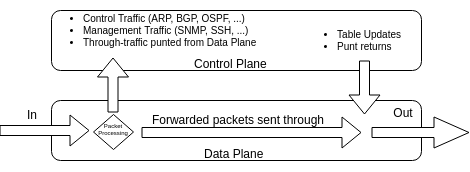
\includegraphics[width=120mm]{content/figs/router_flow_2.png}
\caption{Traffic flow between planes}
\label{fig:router_flow}
\end{figure} 
Network device traffic can be partitioned into two planes\cite{Khosravi_Anderson_2003}: the \textit{Forwarding (or Data) Plane} consists of traffic passing through the device while \textit{Control Plane} traffic has the network element as its destination. We consider the \textit{Management Plane} a subset of the \textit{Control Plane}. Forwarding plane components do the heavy lifting in a network device by connecting incoming traffic to the appropriate outgoing port. When the forwarding element can't identify the correct egress port the packet is sent up to the control plane for a routing solution as shown in Figure \ref{fig:router_flow}. The control plane can request and process information about link status and network topology from peers and update forwarding tables in the data plane in response. 

In conventional network equipment the control and data planes are tightly coupled. That is, the components responsible for forwarding packets are physically located along side the components used to make routing and switching decisions about that traffic. How these systems are laid out in practice varies widely by function and vendor. Figure \ref{fig:router_conventional} depicts a notional router. Line cards house the forwarding engine in Application Specific Integrated Circuits (ASICs), Network Processing Units (NPUs), or even software deployed on virtual machines. Incoming traffic is read off the port into a buffer, the packet header is examined to query the Forwarding Information Base for the destination, the packet processor alters the header as needed, and the packet is forwarded out the appropriate egress port. If the traffic is destined for the device (that is, control or management plane) or if the FIB lookup failed, the packets are queued in the receive path buffer for transfer to the routing engine. The routing engine is typically housed on another line card and connected to the forwarding modules through the backplane or switch fabric. Control plane services are hosted by the network OS running on commodity CPUs. The primary purpose of the control plane service suite is to manipulate the forwarding plane lookup tables based on routing and signalling information it receives. It maintains the Routing Information Base (RIB) used to optimize local FIBs and provides the interface for router management and configuration. 

\begin{figure}[h]
\begin{tabular}{p{0.48\textwidth}p{0.47\textwidth}}
\begin{minipage}{.48\textwidth}
\centering
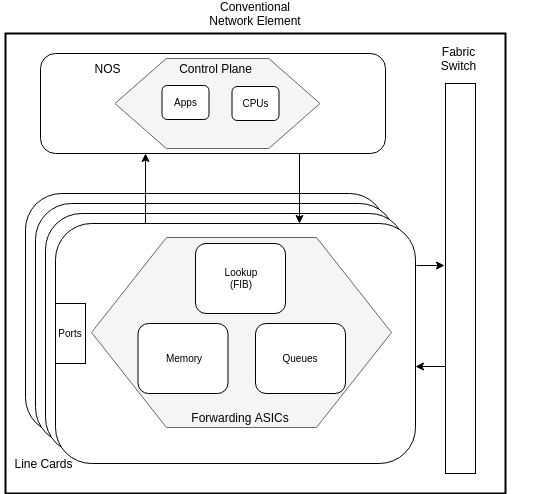
\includegraphics[scale=.4]{content/figs/router_conventional.png}
\caption{Conventional Element}
\label{fig:router_conventional}
%\end{figure} 
\end{minipage}
&
\begin{minipage}{.47\textwidth}
\centering
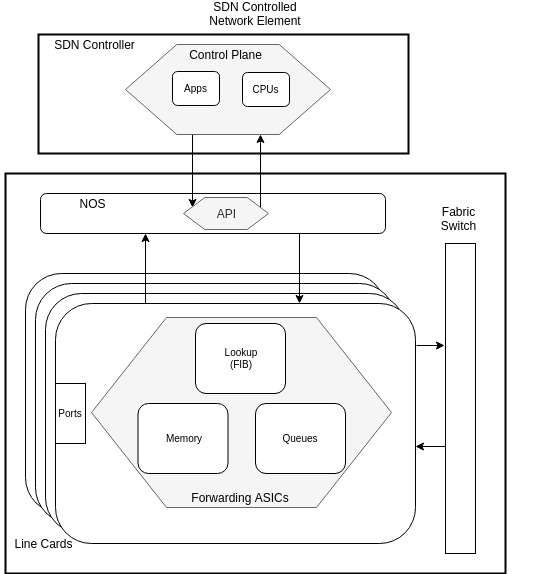
\includegraphics[scale=.4]{content/figs/router_sdn.png}
\caption{SDN Controlled Element}
\label{fig:router_sdn}
\end{minipage}
\end{tabular}
\end{figure}

SDN systems decouple the forwarding and control plane elements further, by centralizing controller functionality outside the data plane's enclosure and introducing a southbound interface with which to alter forwarding tables via API. This allows SDN controllers to scale independently of the forwarding elements and receive state information for all network devices it oversees. Since the complex decision logic has been extracted from the forwarding units, the core elements in SDN are simple switches. The result is a control plane that can optimize the forwarding rules it pushes based on global requirements instead of the limited view available to conventional devices. This also results in a potentially larger attack surface and single point of failure. 

Carrier network architectures can be decomposed into tiers based on functionality and proximity to the end users. The \textit{Access} tier is the forward facing attachment point for a user such as the radio tower a mobile device connects with or the set top box that joins a home network to the ISP. The \textit{Provider Edge } provides the services needed to manage traffic between the various access platforms and the provider core. One or more \textit{Aggregation} layers can be added to consolidate provider edge points based on access density requirements. Finally, the \textit{Provider Core} provides hi speed transit between edge nodes. 

$<$ carrier network diagram here? $>$

% \subsection{Existing Model}\label{subsec:existing_model}
% 
%  MulVal\cite{Ou_Appel_2005} provides an efficient\cite{Rao_1997} Datalog based modeling language and inference engine for vulnerability relationship analysis. The input model consists of configurations for \textbf{hosts} and \textbf{networks}, \textbf{principals} describing user accounts and privileges, rules governing \textbf{interactions}, and access \textbf{policies}. Information about the system under test is either gathered through standard methods such as Nessus, Nmap, and OVAL scans or defined manually for hypothetical data points, and parsed into the global system model using an appropriate adaptor. MulVal can then make inferences about how the entities are able to interact. When provided with a starting and ending node, MulVal enumerates all possible paths an attacker may traverse to compromise the target. The attack graph represents the exploitable vulnerabilities in a system as the set of connected nodes and edges between an attacker’s origin and the target.
 


% \cite{Chowdhary_Pisharody_Huang_2016} Provides a moving target defense solution 

The OSI 7-layer model\cite{Zimmermann_1980} describes network communication as a stack of protocols built on top of a \textit{Physical} transport medium such as copper, optical fiber, or radio. On top of the physical layer are the Layer 2 \textit{Data Link} protocols that facilitate reading and writing frames to and from the given physical circuit including source and destination addressing (\textit{Medium Access Control}), and the protocols that encapsulate/de-encapsulate upper layer packets into the frame format suitable for transmission across the medium (\textit{Logical Link Control}). When a datagram from the upper layers is transmitted to a remote system, it is encapsulated into one or more packets at the \textit{Network} layer, the packets are then encapsulated into frames at the Data Link Layer, and the frames are placed onto the physical medium.  When a frame is received at the destination, it is de-encapsulated and the payload is handed up to the Layer 3 \textit{Network} protocol capable of processing the packet. Encapsulation or de-encapsulation occurs between each layer in the OSI model and  adds processing overhead and increased latency to traffic. Layer 2 traffic is not routable, since routing information like IP address is stored in the Layer 3 header. 

% [width=90mm]\textbf{}
\begin{figure}[ht]
\centering
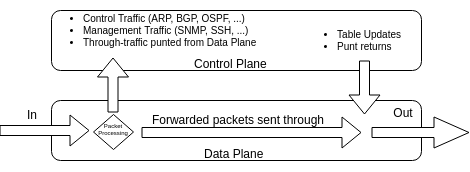
\includegraphics[width=.48\textwidth]{content/figs/router_flow_2.png}
\caption{Traffic flow between planes}
\label{fig:router_flow}
\end{figure} 
Network device traffic can be partitioned into two planes\cite{Khosravi_Anderson_2003}: the \textit{Forwarding (or Data) Plane} consists of traffic passing through the device while \textit{Control Plane} traffic has the network element as its destination. We consider the \textit{Management Plane} a subset of the \textit{Control Plane}. Forwarding plane components do the heavy lifting in a network device by connecting incoming traffic to the appropriate outgoing port. When the forwarding element can't identify the correct egress port the packet is sent up to the control plane for a routing solution as shown in Figure \ref{fig:router_flow}. The control plane can request and process information about link status and network topology from peers and update forwarding tables in the data plane in response. 

In conventional network equipment the control and data planes are tightly coupled. That is, the components responsible for forwarding packets are physically located along side the components used to make routing and switching decisions about that traffic. How these systems are laid out in practice varies widely by function and vendor. Figure \ref{fig:router_conventional} depicts a notional router. Line cards house the forwarding engine in Application Specific Integrated Circuits (ASICs), Network Processing Units (NPUs), or even software deployed on virtual machines. Incoming traffic is read off the port into a buffer, the packet header is examined to query the Forwarding Information Base for the destination, the packet processor alters the header as needed, and the packet is forwarded out the appropriate egress port. If the traffic is destined for the device (that is, control or management plane) or if the FIB lookup failed, the packets are queued in the receive path buffer for transfer to the routing engine. The routing engine is typically housed on another line card and connected to the forwarding modules through the backplane or switch fabric. Control plane services are hosted by the network OS running on commodity CPUs. The primary purpose of the control plane service suite is to manipulate the forwarding plane lookup tables based on routing and signalling information it receives. It maintains the Routing Information Base (RIB) used to optimize local FIBs and provides the interface for router management and configuration. 

\begin{figure}[ht]
\centering
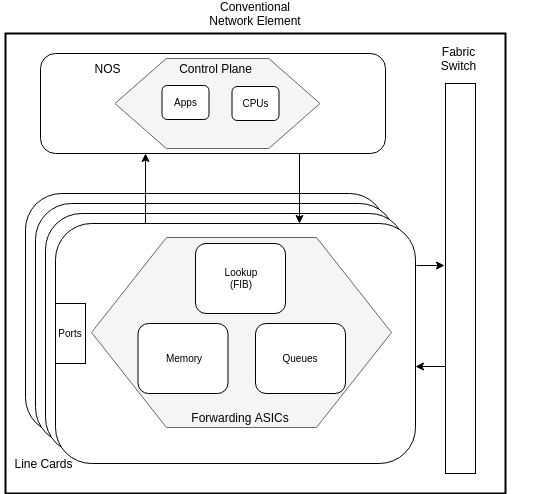
\includegraphics[scale=.45]{content/figs/router_conventional.png}
\caption{Conventional Element}
\label{fig:router_conventional}
\end{figure} 

\begin{figure}[ht]
\centering
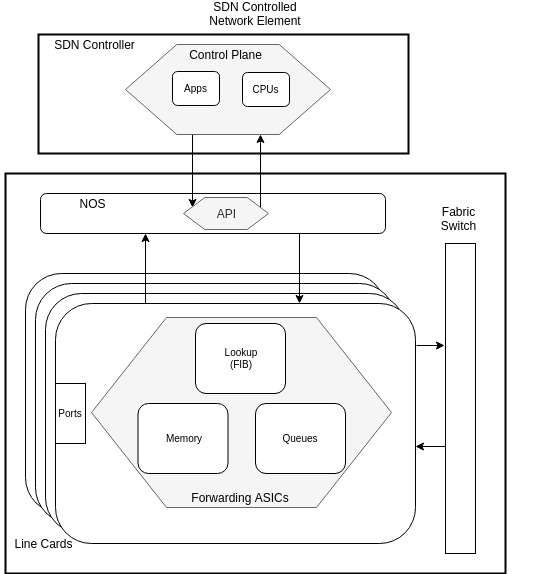
\includegraphics[scale=.45]{content/figs/router_sdn.png}
\caption{SDN Controlled Element}
\label{fig:router_sdn}
% \end{minipage}
% \end{tabular}
\end{figure}

SDN systems decouple the forwarding and control plane elements further, by centralizing controller functionality outside the data plane's enclosure and introducing a southbound interface with which to alter forwarding tables via API. This allows SDN controllers to scale independently of the forwarding elements and receive state information for all network devices it oversees. Since the complex decision logic has been extracted from the forwarding units, the core elements in SDN are simple switches. The result is a control plane that can optimize the forwarding rules it pushes based on global requirements instead of the limited view available to conventional devices. This also results in a potentially larger attack surface and single point of failure. 

Carrier network architectures can be decomposed into tiers based on functionality and proximity to the end users. The \textit{Access} tier is the forward facing attachment point for a user such as the radio tower a mobile device connects with or the set top box that joins a home network to the ISP. The \textit{Provider Edge } provides the services needed to manage traffic between the various access platforms and the provider core. One or more \textit{Aggregation} layers can be added to consolidate provider edge points based on access density requirements. Finally, the \textit{Provider Core} provides hi speed transit between edge nodes. 

$<$ carrier network diagram here? $>$

% \subsection{Existing Model}\label{subsec:existing_model}
% 
%  MulVal\cite{Ou_Appel_2005} provides an efficient\cite{Rao_1997} Datalog based modeling language and inference engine for vulnerability relationship analysis. The input model consists of configurations for \textbf{hosts} and \textbf{networks}, \textbf{principals} describing user accounts and privileges, rules governing \textbf{interactions}, and access \textbf{policies}. Information about the system under test is either gathered through standard methods such as Nessus, Nmap, and OVAL scans or defined manually for hypothetical data points, and parsed into the global system model using an appropriate adaptor. MulVal can then make inferences about how the entities are able to interact. When provided with a starting and ending node, MulVal enumerates all possible paths an attacker may traverse to compromise the target. The attack graph represents the exploitable vulnerabilities in a system as the set of connected nodes and edges between an attacker’s origin and the target.
 


% \cite{Chowdhary_Pisharody_Huang_2016} Provides a moving target defense solution 

The OSI 7-layer model\cite{Zimmermann_1980} describes network communication as a stack of protocols built on top of a \textit{Physical} transport medium such as copper, optical fiber, or radio. On top of the physical layer are the Layer 2 \textit{Data Link} protocols that facilitate reading and writing frames to and from the given physical circuit including source and destination addressing (\textit{Medium Access Control}), and the protocols that encapsulate/de-encapsulate upper layer packets into the frame format suitable for transmission across the medium (\textit{Logical Link Control}). When a datagram from the upper layers is transmitted to a remote system, it is encapsulated into one or more packets at the \textit{Network} layer, the packets are then encapsulated into frames at the Data Link Layer, and the frames are placed onto the physical medium.  When a frame is received at the destination, it is de-encapsulated and the payload is handed up to the Layer 3 \textit{Network} protocol capable of processing the packet. Encapsulation or de-encapsulation occurs between each layer in the OSI model and  adds processing overhead and increased latency to traffic. Layer 2 traffic is not routable, since routing information like IP address is stored in the Layer 3 header. 

% [width=90mm]\textbf{}
\begin{figure}[ht]
\centering
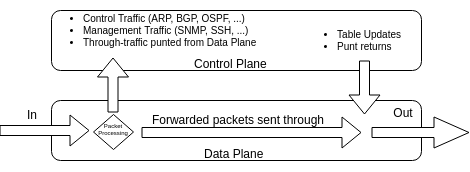
\includegraphics[width=.48\textwidth]{content/figs/router_flow_2.png}
\caption{Traffic flow between planes}
\label{fig:router_flow}
\end{figure} 
Network device traffic can be partitioned into two planes\cite{Khosravi_Anderson_2003}: the \textit{Forwarding (or Data) Plane} consists of traffic passing through the device while \textit{Control Plane} traffic has the network element as its destination. We consider the \textit{Management Plane} a subset of the \textit{Control Plane}. Forwarding plane components do the heavy lifting in a network device by connecting incoming traffic to the appropriate outgoing port. When the forwarding element can't identify the correct egress port the packet is sent up to the control plane for a routing solution as shown in Figure \ref{fig:router_flow}. The control plane can request and process information about link status and network topology from peers and update forwarding tables in the data plane in response. 

In conventional network equipment the control and data planes are tightly coupled. That is, the components responsible for forwarding packets are physically located along side the components used to make routing and switching decisions about that traffic. How these systems are laid out in practice varies widely by function and vendor. Figure \ref{fig:router_conventional} depicts a notional router. Line cards house the forwarding engine in Application Specific Integrated Circuits (ASICs), Network Processing Units (NPUs), or even software deployed on virtual machines. Incoming traffic is read off the port into a buffer, the packet header is examined to query the Forwarding Information Base for the destination, the packet processor alters the header as needed, and the packet is forwarded out the appropriate egress port. If the traffic is destined for the device (that is, control or management plane) or if the FIB lookup failed, the packets are queued in the receive path buffer for transfer to the routing engine. The routing engine is typically housed on another line card and connected to the forwarding modules through the backplane or switch fabric. Control plane services are hosted by the network OS running on commodity CPUs. The primary purpose of the control plane service suite is to manipulate the forwarding plane lookup tables based on routing and signalling information it receives. It maintains the Routing Information Base (RIB) used to optimize local FIBs and provides the interface for router management and configuration. 

\begin{figure}[ht]
\centering
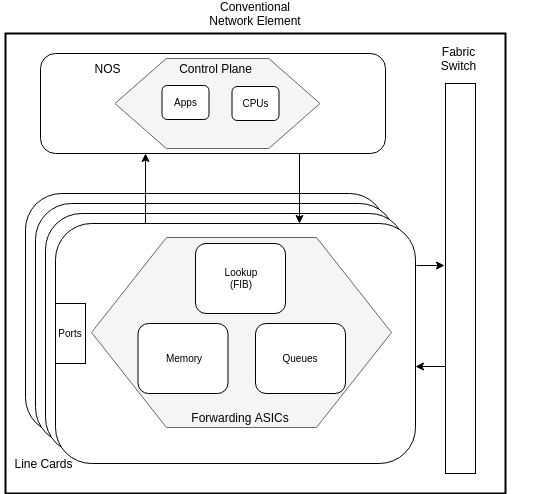
\includegraphics[scale=.45]{content/figs/router_conventional.png}
\caption{Conventional Element}
\label{fig:router_conventional}
\end{figure} 

\begin{figure}[ht]
\centering
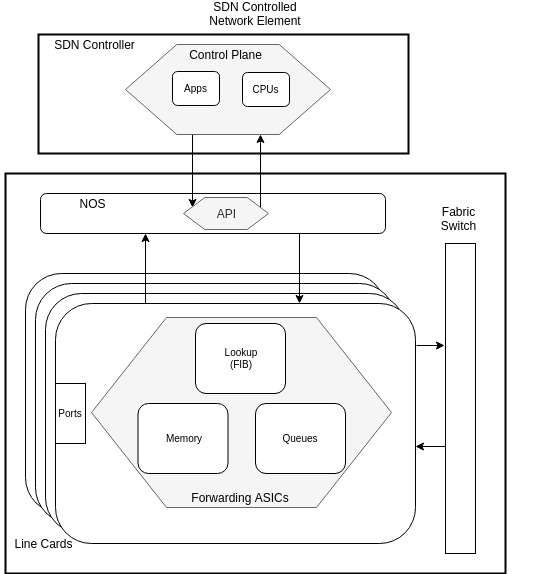
\includegraphics[scale=.45]{content/figs/router_sdn.png}
\caption{SDN Controlled Element}
\label{fig:router_sdn}
% \end{minipage}
% \end{tabular}
\end{figure}

SDN systems decouple the forwarding and control plane elements further, by centralizing controller functionality outside the data plane's enclosure and introducing a southbound interface with which to alter forwarding tables via API. This allows SDN controllers to scale independently of the forwarding elements and receive state information for all network devices it oversees. Since the complex decision logic has been extracted from the forwarding units, the core elements in SDN are simple switches. The result is a control plane that can optimize the forwarding rules it pushes based on global requirements instead of the limited view available to conventional devices. This also results in a potentially larger attack surface and single point of failure. 

Carrier network architectures can be decomposed into tiers based on functionality and proximity to the end users. The \textit{Access} tier is the forward facing attachment point for a user such as the radio tower a mobile device connects with or the set top box that joins a home network to the ISP. The \textit{Provider Edge } provides the services needed to manage traffic between the various access platforms and the provider core. One or more \textit{Aggregation} layers can be added to consolidate provider edge points based on access density requirements. Finally, the \textit{Provider Core} provides hi speed transit between edge nodes. 

$<$ carrier network diagram here? $>$

% \subsection{Existing Model}\label{subsec:existing_model}
% 
%  MulVal\cite{Ou_Appel_2005} provides an efficient\cite{Rao_1997} Datalog based modeling language and inference engine for vulnerability relationship analysis. The input model consists of configurations for \textbf{hosts} and \textbf{networks}, \textbf{principals} describing user accounts and privileges, rules governing \textbf{interactions}, and access \textbf{policies}. Information about the system under test is either gathered through standard methods such as Nessus, Nmap, and OVAL scans or defined manually for hypothetical data points, and parsed into the global system model using an appropriate adaptor. MulVal can then make inferences about how the entities are able to interact. When provided with a starting and ending node, MulVal enumerates all possible paths an attacker may traverse to compromise the target. The attack graph represents the exploitable vulnerabilities in a system as the set of connected nodes and edges between an attacker’s origin and the target.
 


% \cite{Chowdhary_Pisharody_Huang_2016} Provides a moving target defense solution 

The OSI 7-layer model\cite{Zimmermann_1980} describes network communication as a stack of protocols built on top of a \textit{Physical} transport medium such as copper, optical fiber, or radio. On top of the physical layer are the Layer 2 \textit{Data Link} protocols that facilitate reading and writing frames to and from the given physical circuit including source and destination addressing (\textit{Medium Access Control}), and the protocols that encapsulate/de-encapsulate upper layer packets into the frame format suitable for transmission across the medium (\textit{Logical Link Control}). When a datagram from the upper layers is transmitted to a remote system, it is encapsulated into one or more packets at the \textit{Network} layer, the packets are then encapsulated into frames at the Data Link Layer, and the frames are placed onto the physical medium.  When a frame is received at the destination, it is de-encapsulated and the payload is handed up to the Layer 3 \textit{Network} protocol capable of processing the packet. Encapsulation or de-encapsulation occurs between each layer in the OSI model and  adds processing overhead and increased latency to traffic. Layer 2 traffic is not routable, since routing information like IP address is stored in the Layer 3 header. 

% [width=90mm]\textbf{}
\begin{figure}[ht]
\centering
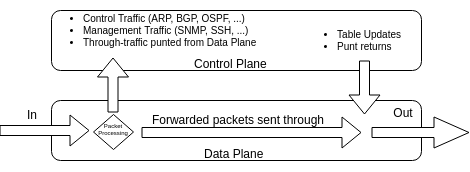
\includegraphics[width=.48\textwidth]{content/figs/router_flow_2.png}
\caption{Traffic flow between planes}
\label{fig:router_flow}
\end{figure} 
Network device traffic can be partitioned into two planes\cite{Khosravi_Anderson_2003}: the \textit{Forwarding (or Data) Plane} consists of traffic passing through the device while \textit{Control Plane} traffic has the network element as its destination. We consider the \textit{Management Plane} a subset of the \textit{Control Plane}. Forwarding plane components do the heavy lifting in a network device by connecting incoming traffic to the appropriate outgoing port. When the forwarding element can't identify the correct egress port the packet is sent up to the control plane for a routing solution as shown in Figure \ref{fig:router_flow}. The control plane can request and process information about link status and network topology from peers and update forwarding tables in the data plane in response. 

In conventional network equipment the control and data planes are tightly coupled. That is, the components responsible for forwarding packets are physically located along side the components used to make routing and switching decisions about that traffic. How these systems are laid out in practice varies widely by function and vendor. Figure \ref{fig:router_conventional} depicts a notional router. Line cards house the forwarding engine in Application Specific Integrated Circuits (ASICs), Network Processing Units (NPUs), or even software deployed on virtual machines. Incoming traffic is read off the port into a buffer, the packet header is examined to query the Forwarding Information Base for the destination, the packet processor alters the header as needed, and the packet is forwarded out the appropriate egress port. If the traffic is destined for the device (that is, control or management plane) or if the FIB lookup failed, the packets are queued in the receive path buffer for transfer to the routing engine. The routing engine is typically housed on another line card and connected to the forwarding modules through the backplane or switch fabric. Control plane services are hosted by the network OS running on commodity CPUs. The primary purpose of the control plane service suite is to manipulate the forwarding plane lookup tables based on routing and signalling information it receives. It maintains the Routing Information Base (RIB) used to optimize local FIBs and provides the interface for router management and configuration. 

\begin{figure}[ht]
\centering
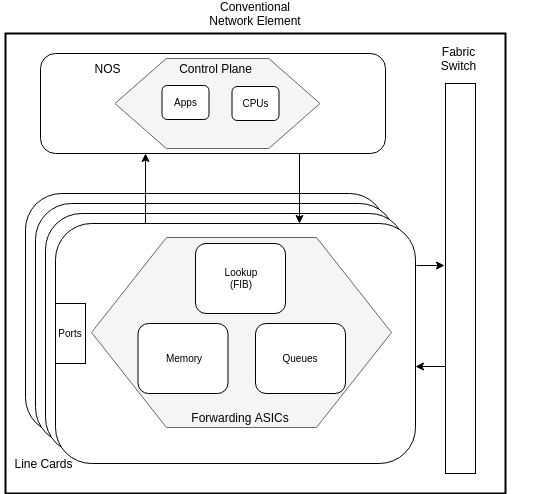
\includegraphics[scale=.45]{content/figs/router_conventional.png}
\caption{Conventional Element}
\label{fig:router_conventional}
\end{figure} 

\begin{figure}[ht]
\centering
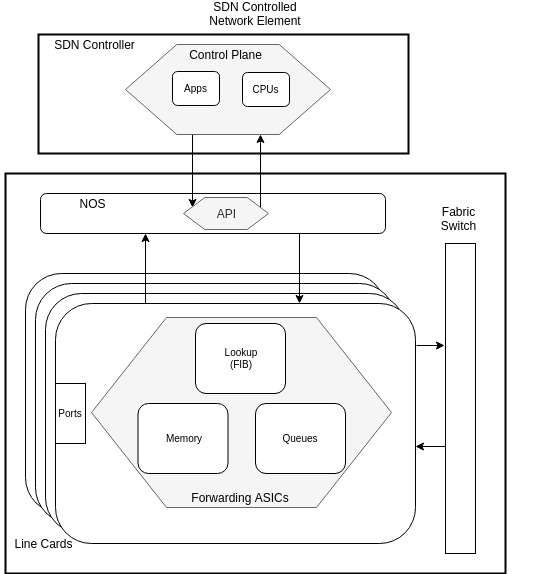
\includegraphics[scale=.45]{content/figs/router_sdn.png}
\caption{SDN Controlled Element}
\label{fig:router_sdn}
% \end{minipage}
% \end{tabular}
\end{figure}

SDN systems decouple the forwarding and control plane elements further, by centralizing controller functionality outside the data plane's enclosure and introducing a southbound interface with which to alter forwarding tables via API. This allows SDN controllers to scale independently of the forwarding elements and receive state information for all network devices it oversees. Since the complex decision logic has been extracted from the forwarding units, the core elements in SDN are simple switches. The result is a control plane that can optimize the forwarding rules it pushes based on global requirements instead of the limited view available to conventional devices. This also results in a potentially larger attack surface and single point of failure. 

Carrier network architectures can be decomposed into tiers based on functionality and proximity to the end users. The \textit{Access} tier is the forward facing attachment point for a user such as the radio tower a mobile device connects with or the set top box that joins a home network to the ISP. The \textit{Provider Edge } provides the services needed to manage traffic between the various access platforms and the provider core. One or more \textit{Aggregation} layers can be added to consolidate provider edge points based on access density requirements. Finally, the \textit{Provider Core} provides hi speed transit between edge nodes. 

$<$ carrier network diagram here? $>$

% \subsection{Existing Model}\label{subsec:existing_model}
% \input{content/contrib/inrfa/infra_model.tex}

% \subsection{Layer 2}\label{subsec:infra_l2}
% \input{content/contrib/inrfa/layer2.tex}
% \subsection{Layer 3}\label{subsec:infra_l3}
% \input{content/contrib/inrfa/layer3.tex}


% \begin{figure}[H]
% \begin{tabular}{p{0.5\textwidth}p{0.5\textwidth}}
% \begin{minipage}{.5\textwidth}
% \begin{lstlisting}[style=datalog, label={lst:preds}, caption={preds.P \cite{Ou_Boyer_McQueen_2006}}]

% /******************************************************/
% /****         Predicates Declaration              *****/
% /******************************************************/

% primitive(inCompetent(_principal)).
% primitive(competent(_principal)).
% primitive(clientProgram(_host, _programname)).
% primitive(vulExists(_host, _vulID, _program)).
% primitive(vulProperty(_vulID, _range, _consequence)).
% primitive(hacl(_src, _dst, _prot, _port)).
% primitive(attackerLocated(_host)).
% primitive(hasAccount(_principal, _host, _account)).
% primitive(networkServiceInfo(_host, _program, _protocol, _port, _user)).
% primitive(setuidProgramInfo(_host, _program, _owner)).
% primitive(nfsExportInfo(_server, _path, _access, _client)).
% primitive(nfsMounted(_client, _clientpath, _server, _serverpath, _access)).
% primitive(localFileProtection(_host, _user, _access, _path)).
% primitive(dependsOn(_h, _program, _library)).
% primitive(installed(_h, _program)).
% primitive(bugHyp(_,_,_,_)).
% primitive(vulExists(_machine,_vulID,_program,_range,_consequence)).
% primitive(canAccessFile(_host, _user, _access, _path)).
% primitive(isWebServer(_host)).
% meta(cvss(_vulID, _ac)).


% derived(execCode(_host, _user)).
% derived(netAccess(_machine,_protocol,_port)).
% derived(canAccessHost(_host)).
% derived(accessFile(_machine,_access,_filepath)).
% derived(accessMaliciousInput(_host, _principal, _program)).
% derived(principalCompromised(_victim)).
% derived(dos(_host)).
% derived(logInService(_host, _protocol, _port)).

% meta(attackGoal(_)).
% meta(advances(_, _)).

% /******************************************************/
% /****         Tabling Predicates                  *****/
% /*   All derived predicates should be tabled          */
% /******************************************************/

% :- table execCode/2.
% :- table netAccess/3.
% :- table canAccessHost/1.
% :- table canAccessFile/4.
% :- table accessFile/3.
% :- table principalCompromised/1.
% :- table vulExists/5.
% :- table logInService/3.
% \end{lstlisting}
% \label{fig:eg_net01}
% %\end{figure} 
% \end{minipage}
% &
% \begin{minipage}{.5\textwidth}
% % \begin{adjustbox}{width=\textwidth}
% \begin{lstlisting}[style=datalog, label={lst:rules}, caption={input.P \cite{Ou_Boyer_McQueen_2006}}]

% /******************************************************/
% /****         Interaction Rules                   *****/
% /******************************************************/

% /****** Section execCode ******
% interaction_rule(
%   (execCode(H, Perm) :-
% 	hasAccount(P, H, Perm)),
%   rule_desc('Insider threat', 1)).
% */

% interaction_rule(
%   (execCode(Host, Perm) :-
% 	principalCompromised(Victim),
% 	hasAccount(Victim, Host, Perm),
% 	canAccessHost(Host)),
%   rule_desc('When a principal is compromised any machine he has an account on will also be compromised',
%   0.5)).

% interaction_rule(
%   (execCode(Host, root) :-
% 	execCode(Host, _Perm2),
% 	vulExists(Host, _, Software, localExploit, privEscalation)),
%   rule_desc('local exploit',
%   1.0)).

% interaction_rule(
%   (execCode(H, Perm) :-
% 	vulExists(H, _, Software, remoteExploit, privEscalation),
% 	networkServiceInfo(H, Software, Protocol, Port, Perm),
% 	netAccess(H, Protocol, Port)),
%   rule_desc('remote exploit of a server program',
%   1.0)).

% interaction_rule(
%   (execCode(H, Perm) :-
%         vulExists(H, _, Software, remoteClient, privEscalation),
% 	hasAccount(Victim, H, Perm),
%         accessMaliciousInput(H, Victim, Software)),
%   rule_desc('remote exploit for a client program',
%   0.5)).

% interaction_rule(
%   (execCode(H, root) :-
% 	accessFile(H, write, _Path)),
%   rule_desc('Trojan horse installation',
%   0.8)).

% /* Singleton variable at head
% interaction_rule(
%  (execCode( Attacker, Host, _) :-
%   execCode(Attacker, Host, root)),
%   'execution at any level if root execution').
% */

% \end{lstlisting}
% % \end{adjustbox}
% \end{minipage}
% \end{tabular}
% \end{figure}




% \begin{figure}[H]
% \begin{tabular}{p{0.5\textwidth}p{0.5\textwidth}}
% \begin{minipage}{.5\textwidth}
% \begin{lstlisting}[style=datalog, label={lst:preds}2, caption={preds.P \cite{Ou_Boyer_McQueen_2006}}]


% /******** Section netAccess ********/
% /* accessing a host through network according to a hacl policy.
%   For now we assume that every user on a local
%   machine has access to network. this may change
%   later. */
% interaction_rule(
%   (netAccess(H2, Protocol, Port) :-
% 	execCode(H1, _Perm),  /* Any permission level */
% 	advances(H1, H2),
%     hacl(H1, H2, Protocol, Port)),
%   rule_desc('multi-hop access',
%   0.5)).

% interaction_rule(
%   (netAccess(H, Protocol, Port) :-
% 	attackerLocated(Zone),
% 	hacl(Zone, H, Protocol, Port)),
%   rule_desc('direct network access',
%   1.0)).

% interaction_rule(
%   (netAccess(H, Protocol, Port) :-
% 	attackerLocated(H)),
%   rule_desc('direct on-host access',
%   1.0)).



% /****** Section canAccessHost ******/
% interaction_rule(
%   (canAccessHost(H) :-
% 	execCode(H, _Perm)),
%   rule_desc('Access a host through executing code on the machine',
%   1.0)).

% interaction_rule(
%   (canAccessHost(H) :-
% 	logInService(H, Protocol, Port),
% 	netAccess(H, Protocol, Port)),
%   rule_desc('Access a host through a log-in service',
%   1.0)).


% /******** Section accessFile ********/
% interaction_rule(
%   (accessFile(H, Access, Path) :-
% 	execCode(H, Usr),
% 	canAccessFile(H, Usr, Access, Path)),
%   rule_desc('execCode implies file access',
%   1.0)).


% /****** Section principalCompromised ******/
% interaction_rule(
%   (principalCompromised(Victim) :-
% 	hasAccount(Victim, H, _Perm),
% 	execCode(H, root)),
%   rule_desc('password sniffing',
%   0.8)).

% interaction_rule(
%   (principalCompromised(Victim) :-
% 	hasAccount(Victim, H, User),
% 	execCode(H, User)),
%   rule_desc('password sniffing',
%   0.8)).



% \end{lstlisting}
% \label{fig:eg_net01}
% %\end{figure} 
% \end{minipage}
% &
% \begin{minipage}{.5\textwidth}
% % \begin{adjustbox}{width=\textwidth}
% \begin{lstlisting}[style=datalog, label={lst:preds4}, caption={input.P \cite{Ou_Boyer_McQueen_2006}}]

% /*
% interaction_rule(
%   (principalCompromised(Victim) :-
% 	inCompetent(Victim)),
%   rule_desc('incompetent user',
%   0.2)).
% */

% /********************************************************/
% /*      Software specific knowledge                     */
% /********************************************************/

% /*
% explain(logInService(H, Protocol, Port), Text) :-
% 	fmt_write_string(Text,
%   "There is a login service running under protocol %S and port %S on host %S.", args(Protocol, Port, H)).
% */



% /***************** Section ssh **********************/
% interaction_rule(
%   (logInService(H, Protocol, Port) :-
% 	networkServiceInfo(H, sshd, Protocol, Port, _)),
%   rule_desc('',
%   1)).

% interaction_rule(
%   (logInService(H, Protocol, Port) :-
% 	networkServiceInfo(H, vpnService, Protocol, Port, _)),
%   rule_desc('',
%   1)).


% /**************** Section  nfs *****************/
% /* Principal P can access files on a NFS server if the files
%   on the server are mounted at a client and he can access the
%   files on the client side */
% interaction_rule(
%   (accessFile(Server, Access, ServerPath) :-
% 	nfsMounted(Client, ClientPath, Server, ServerPath, Access),
% 	accessFile(Client, Access, ClientPath)),
%   rule_desc('NFS semantics',
%   1)).


% /* Principal P can access files on a NFS client if the files
%   on the server are mounted at the client and he can access the
%   files on the server side */
% interaction_rule(
%   (accessFile(Client, Access, ClientPath) :-
% 	nfsMounted(Client, ClientPath, Server, ServerPath, read),
% 	accessFile(Server, Access, ServerPath)),
%   rule_desc('NFS semantics',
%   1)).


% interaction_rule(
%   (accessFile(Server, Access, Path) :-
% 	execCode(Client, _User),
%     nfsExportInfo(Server, Path, Access, Client),
%     hacl(Client, Server, nfsProtocol, nfsPort)),
%   rule_desc('NFS shell',
%   0.8)).
% \end{lstlisting}
% % \end{adjustbox}
% \end{minipage}
% \end{tabular}
% \end{figure}



% \begin{figure}[H]
% \begin{tabular}{p{0.5\textwidth}p{0.5\textwidth}}
% \begin{minipage}{.5\textwidth}
% \begin{lstlisting}[style=datalog, label={lst:preds5}, caption={preds.P \cite{Ou_Boyer_McQueen_2006}}]



% interaction_rule(
%   (canAccessFile(H, Usr, Acc, Path) :-
% 	localFileProtection(H, Usr, Acc, Path)),
%   rule_desc('',
%   1)).

% /* Singleton variable in head
% interaction_rule(
%   (canAccessFile(_H, root, _Access, _Path)),
%   'root has arbitrary access').
% */



% interaction_rule((vulExists(H, ID, Sw, Range, Consequence):-
% 	        vulExists(H, ID, Sw),
% 		vulProperty(ID, Range, Consequence)),
%              rule_desc('',
%              1)).

% interaction_rule((vulExists(H, _ID, Sw, Range, Consequence):-
% 	        bugHyp(H, Sw, Range, Consequence)),
%              rule_desc('Introducing hypothetical bug',
%              1)).


% interaction_rule((vulExists(H, ID, Sw, Range, Consequence):-
% 	        vulExists(H, ID, Library, Range, Consequence),
% 		dependsOn(H, Sw, Library)),
%              rule_desc('Library bug',
%              1)).

% interaction_rule(
%   (accessMaliciousInput(H, Victim, Software) :-
%      inCompetent(Victim),
%      hacl(H, MaliciousMachine, httpProtocol, httpPort),
%      attackerLocated(MaliciousMachine)),
%   rule_desc('Browsing a malicious website', 0.8)).

% interaction_rule(
%   (accessMaliciousInput(H, Victim, Software) :-
%      competent(Victim),
%      hacl(H, MaliciousMachine, httpProtocol, httpPort),
%      attackerLocated(MaliciousMachine)),
%   rule_desc('Browsing a malicious website', 0.1)).


% \end{lstlisting}
% \label{fig:eg_net01}
% %\end{figure} 
% \end{minipage}
% &
% \begin{minipage}{.5\textwidth}
% % \begin{adjustbox}{width=\textwidth}
% \begin{lstlisting}[style=datalog, label={lst:preds6}, caption={input.P \cite{Ou_Boyer_McQueen_2006}}]


% interaction_rule(
%   (accessMaliciousInput(H, Victim, Software) :-
%      inCompetent(Victim),
%      isWebServer(CompromisedMachine),
%      hacl(H, CompromisedMachine, httpProtocol, httpPort),
%      execCode(CompromisedMachine, _)),
%   rule_desc('Browsing a compromised website', 0.4)).


% /*
% interaction_rule(
%   (canAccessMaliciousInput(H, Browser) :-
%      installed(H, Browser),
%      isWebBrowser(Browser)),
%   rule_desc('A browser can potentially access malicious input',
%   1)).


% interaction_rule(
%   (canAccessMaliciousInput(H, Software) :-
% 	vulExists(H, _, Software, remoteClient, privEscalation),
% 	inCompetent(Victim),
% 	hasAccount(Victim, H, _Perm)),
%   rule_desc('A remote client vulnerability can potentially access malicious input from a host used by careless user',
%   1)).



% interaction_rule(
%   (canAccessMaliciousInput(H, Browser) :-
%      installed(H, Browser),
%      isWebBrowser(Browser),
%      hacl(H, MaliciousMachine, httpProtocol, httpPort),
%      attackerLocated(MaliciousMachine)),
%   rule_desc('Browsing a malicious website',
%   1)).

% interaction_rule(
%   (canAccessMaliciousInput(H, Browser) :-
%      installed(H, Browser),
%      isWebBrowser(Browser),
%      hacl(H, CompromisedMachine, httpProtocol, httpPort),
%      execCode(CompromisedMachine, _)),
%   rule_desc('Browsing a compromised website',
%   0.4)).

% interaction_rule(
%   (canAccessMaliciousInput(H, EmailClientSoftware) :-
%      installed(H, EmailClientSoftware),
%      isEmailClient(EmailClientSoftware),
%      isEmailServer(EmailServerSoftware),
%      hacl(H, EmailServer, EmailProtocol, EmailPort),
%      networkServiceInfo(EmailServer, EmailServerSoftware,
%                                 EmailProtocol, EmailPort, _Perm)),
%   rule_desc('receive an email message',
%   0.4)).

% \end{lstlisting}
% % \end{adjustbox}
% \end{minipage}
% \end{tabular}
% \end{figure}




% \begin{figure}[H]
% \begin{tabular}{p{0.5\textwidth}p{0.5\textwidth}}
% \begin{minipage}{.5\textwidth}
% \begin{lstlisting}[style=datalog, label={lst:tr_rules1}, caption={iav.P \cite{Ou_Boyer_McQueen_2006}}]


% /*
% IAV Network State Model
% */


% /*
%   attacker is at the customer edge or internet 
%   pe1 is CRS with vuln CVE-2012-1342 (BGP overflow remote code execution)
%   target is core router p3 control plane code execution

% _c control plane interface
% _d data plane interface
% _m management interface
% */
% attackerLocated(ce1).
% attackGoal(execCode(p3_c, _)).

% /*
% Customer Edge devices attach to Provider Edges
% control plane to exchange routing tables/VRFs
% through BGP
% */
% /* BGP b/t customer and provider edge */
% /* update 20160425: data and control from customer on same PE port */
% /*hacl(ce1, pe1_c,  tcp, 179).*/
% hacl(ce1, pe1_d,  _, _). 
% hacl(pe1_d, pe1_c,  _, _).

% /* 
% Customer data flows through PE data plane on predefined label switched path (MPLS tunnel)
% */

% /*
% Provider Edge devices talk to other PEs
% BGP b/t provider edges control plane to
% exchange client VRFs for tunnel endpoints 
% */
% hacl(pe1_c, pe2_c,  TCP, 179).
% hacl(pe1_c, pe4_c, TCP, 179).
% hacl(pe2_c, pe3_c, TCP, 179).
% hacl(pe2_c, pe1_c, TCP, 179).
% hacl(pe3_c, pe4_c,  TCP, 179).
% hacl(pe3_c, pe2_c,  TCP, 179).
% hacl(pe4_c, pe1_c,  TCP, 179).
% /*hacl(pe4_c, pe3_c,  TCP, 179). handle Cycles*/

% /*
% PEs also talk to neighbor P nodes over LDP 
% */
% hacl(pe1_c, p1_c,  TCP, 646).
% hacl(pe2_c, p1_c, TCP, 646).
% hacl(pe3_c, p3_c,  TCP, 646).
% hacl(pe4_c, p3_c,  TCP, 646).

% \end{lstlisting}
% \label{fig:eg_net01}
% %\end{figure} 
% \end{minipage}
% &
% \begin{minipage}{.5\textwidth}
% % \begin{adjustbox}{width=\textwidth}
% \begin{lstlisting}[style=datalog, label={lst:tr_rules2}, caption={input.P \cite{Ou_Boyer_McQueen_2006}}]

% /* 
% allow PEs to speak BGP with Aggregation P's 
% (this is to give us an attack path on the control plane, 
% other wise no path would exist)
%  */
% hacl(pe1_c, p1_c,  TCP, 179).
% hacl(pe2_c, p1_c, TCP, 179).
% hacl(pe3_c, p3_c, TCP, 179).
% hacl(pe4_c, p3_c,  TCP, 179).
% /* 
% hacl(pe1_c, p1_c,  TCP, 179).
% hacl(pe2_c, p1_c, TCP, 179).
% hacl(p1_c, pe1_c,  TCP, 179).
% hacl(p1_c, pe1_c, TCP, 179).
% hacl(p3_c, pe3_c, TCP, 179).
% hacl(p3_c, pe4_c,  TCP, 179).
% hacl(pe3_c, p3_c, TCP, 179).
% hacl(pe4_c, p3_c,  TCP, 179).
% */

% /*
% Core P nodes speak LDP to each other to establish LSPs
% The VPN tunnel over an LSP can be configured statically or dynamically with TE bindings.
% We assume static for now. 
% */
% /* allow control messages through LDP */
% hacl(p1_c, p2_c,  TCP, 646).
% hacl(p1_c, p4_c, TCP, 646).
% hacl(p1_c, p3_c, TCP, 646).
% hacl(p2_c, p3_c,  TCP, 646).
% hacl(p4_c, p3_c,  TCP, 646).

% /* 
% assume our LSP tunnel is configured:
% PE1 -> P1 -> P3 -> PE3
% data flow is one way (another tunnel needed for return traffic)
%  */
% hacl(pe1_d, p1_d,  _, _).
% hacl(p1_d, p3_d, _, _).
% hacl(p3_d, pe3_d, _, _).

% /* 
% P's don't speak BGP to other Ps
% (although OSPF might be used for neighbor/LDP exchange)
% */
% /*
% hacl(p1_c, p2_c, TCP, 179).
% hacl(p1_c, p4_c, TCP, 179).
% hacl(p2_c, p3_c,  TCP, 179).
% hacl(p4_c, p3_c,  TCP, 179).
% */


% \end{lstlisting}
% % \end{adjustbox}
% \end{minipage}
% \end{tabular}
% \end{figure}

% \begin{figure}[H]
% \begin{tabular}{p{0.5\textwidth}p{0.5\textwidth}}
% \begin{minipage}{.5\textwidth}
% \begin{lstlisting}[style=datalog, label={lst:transition_model1}, caption={iav.P \cite{Ou_Boyer_McQueen_2006}}]
% /*
% Management Plane interfaces allow SSH, Telnet, SNMP, NTP
% to all network elements
% just adding SSH for now to avoid clutter 
% (can't separate multiple ports with | )
% */
% /* 
% hacl(pe1_m, _,  tcp, 22).
% hacl(pe2_m, _,  tcp, 22).
% hacl(pe3_m, _,  tcp, 22).
% hacl(pe3_m, _,  tcp, 22).
% hacl(p1_m, _,  tcp, 22).
% hacl(p2_m, _,  tcp, 22).
% hacl(p3_m, _,  tcp, 22).
% hacl(p4_m, _,  tcp, 22).
% */
% /*
% hacl(H, H, _, _).
% */
% /*
% Vulnerability Definitions
% */
% /* 
% PE's can be:
% Cisco 12000 (IOS v12)
% Cisco ASR 9000 (IOS XR 4.1)
% Cisco CRS1 (IOS XR 4.3)
% */
% /* BGP exploit lets attacker escalate privilege on attached PE's control interface 
% CVE-2012-1342, cvss=5
% From there attacker can execute remote code on other PEs with
% CVE-2013-1234, cvss=4 
% */
% /*
% vulExists(pe1_c, 'CVE-2012-1342', bgp).
% vulExists(pe1_d, 'CVE-2012-1342', _).*/ /* CE ingress control/data same port */
% /*vulExists(pe2_c, 'CVE-2012-1342', bgp).
% vulExists(pe3_c, 'CVE-2012-1342', bgp).
% vulExists(pe4_c, 'CVE-2012-1342', bgp).
% vulExists(p1_c, 'CVE-2012-1342', bgp).
% vulExists(p3_c, 'CVE-2012-1342', bgp).
% vulProperty( 'CVE-2012-1342', remoteExploit, privEscalation).
% networkServiceInfo(pe1_c , bgp, TCP, 179, root).
% networkServiceInfo(pe2_c , bgp, TCP, 179, root).
% networkServiceInfo(pe3_c , bgp, TCP, 179, root).
% networkServiceInfo(pe4_c , bgp, TCP, 179, root).
% networkServiceInfo(p1_c , bgp, TCP, 179, root).
% networkServiceInfo(p3_c , bgp, TCP, 179, root).
% */

% vulExists(pe1_c, 'CVE-2012-1342', bgp).
% vulExists(pe1_d, 'CVE-2007-5381', _). /* CE ingress control/data same port */
% vulExists(pe2_c, 'CVE-2013-1234', bgp).
% vulExists(pe3_c, 'CVE-2013-1234', bgp).
% vulExists(pe4_c, 'CVE-2013-1234', bgp).
% vulExists(p1_c, 'CVE-2013-1234', bgp).
% vulExists(p3_c, 'CVE-2013-1234', bgp).
% vulProperty( 'CVE-2012-1342', remoteExploit, privEscalation).
% vulProperty( 'CVE-2013-1234', remoteExploit, privEscalation).
% networkServiceInfo(pe1_c , bgp, TCP, 179, root).
% networkServiceInfo(pe1_d , _, _, _, root). /* control & data on the same CE ingress port */
% networkServiceInfo(pe2_c , bgp, TCP, 179, root).
% networkServiceInfo(pe3_c , bgp, TCP, 179, root).
% networkServiceInfo(pe4_c , bgp, TCP, 179, root).
% networkServiceInfo(p1_c , bgp, TCP, 179, root).
% networkServiceInfo(p3_c , bgp, TCP, 179, root).
% \end{lstlisting}
% \label{fig:eg_net01}
% %\end{figure} 
% \end{minipage}
% &
% \begin{minipage}{.5\textwidth}
% % \begin{adjustbox}{width=\textwidth}
% \begin{lstlisting}[style=datalog, label={lst:transition_model2}, caption={trans.P \cite{Ou_Boyer_McQueen_2006}}]
% /* 
% Even if the P nodes have the same vulnerabilities as the current architecture, address space isolation prevents attackers from directly addressing these elements.
% CVE-2007-5381, CVSS=9.3 (actually LPD vuln)
% */
% vulExists(p1_d, 'CVE-2007-5381', rsvp).
% vulExists(p2_d, 'CVE-2007-5381', rsvp).
% vulExists(p3_d, 'CVE-2007-5381', rsvp).
% vulExists(p4_d, 'CVE-2007-5381', rsvp).
% vulProperty( 'CVE-2007-5381', remoteExploit, privEscalation).
% /*
% networkServiceInfo(p3_d , rsvp, TCP, 3455, root).
% networkServiceInfo(p1_d , _, _, _, _).
% networkServiceInfo(p2_d , _, _, _, _).
% networkServiceInfo(p4_d , _, _, _, _).
% hacl(p3_d, p3_c,  _, _). */ /*this is the result of the exploit */

% /* Remote code execution allows attacker to move from control -> management plane */
% /*
% vulExists(pe2_m, 'CVE-2007-5381', _).
% vulProperty( 'CVE-2007-5381', remoteExploit, privEscalation).
% networkServiceInfo(pe2_m , _, _, _, _).

% vulExists(pe3_c, 'CVE-2011-4012', _).
% vulProperty( 'CVE-2011-4012', remoteExploit, privEscalation).
% networkServiceInfo(pe3_c , bgp, tcp, 179, root).

% vulExists(pe4_c, 'CVE-2015-0694', _).
% vulProperty( 'CVE-2015-0694', remoteExploit, privEscalation).
% networkServiceInfo(pe4_c , _, _, _, _).
% */

% /*  
% P's can be:
% Cisco CRS1 (IOS XR 4.3)
% */

% /*
% Assuming aggregation (P1,P3) run BGP but core (P2,P4) don't
% This gives a common attack path between the 3 models,
% otherwise IAV would have no attack paths (we could introduce another PE->Aggregation vuln)
% 'CVE-2009-2048' - CVSS 3.5
% */
% vulExists(p1_c, 'CVE-2009-2048',_).
% vulProperty('CVE-2009-2048', remoteExploit, privEscalation).
% networkServiceInfo(p1_c , bgp, TCP, 179, root).
% vulExists(p3_c, 'CVE-2009-2048',_).
% vulProperty('CVE-2009-2048', remoteExploit, privEscalation).
% networkServiceInfo(p3_c ,  bgp, TCP, 179, root).
% /*
% vulExists(p2_c, 'CVE-2009-2048',_).
% vulProperty('CVE-2009-2048', remoteExploit, privEscalation).
% networkServiceInfo(p2_c , _, _, _, _).
% vulExists(p4_c, 'CVE-2009-2048',_).
% vulProperty('CVE-2009-2048', remoteExploit, privEscalation).
% networkServiceInfo(p4_c , bgp, TCP, 179, root).
% */

% /*  
% RR's can be:
% Juniper M320 (JunOS 13.2)
% Can add these between sites/AS's if vulnerabilities are identified
% */

% \end{lstlisting}
% % \end{adjustbox}
% \end{minipage}
% \end{tabular}
% \end{figure}









% \begin{figure}[H]
% \begin{tabular}{p{0.5\textwidth}p{0.5\textwidth}}
% \begin{minipage}{.5\textwidth}
% \begin{lstlisting}[style=datalog, label={lst:tr_rules1}, caption={iav.P \cite{Ou_Boyer_McQueen_2006}}]

% \end{lstlisting}
% \label{fig:eg_net01}
% %\end{figure} 
% \end{minipage}
% &
% \begin{minipage}{.5\textwidth}
% % \begin{adjustbox}{width=\textwidth}
% \begin{lstlisting}[style=datalog, label={lst:tr_rules2}, caption={input.P \cite{Ou_Boyer_McQueen_2006}}]
% .
% \end{lstlisting}
% % \end{adjustbox}
% \end{minipage}
% \end{tabular}
% \end{figure}


% % \begin{figure}[H]
% % \begin{tabular}{p{0.5\textwidth}p{0.5\textwidth}}
% % \begin{minipage}{.5\textwidth}
% % \begin{lstlisting}[style=datalog, label={lst:tr_rules1}, caption={preds.P \cite{Ou_Boyer_McQueen_2006}}]
% % :-(mvTrc(execCode(_h3708,_h3709,0)),','(mvTrc(principalCompromised(_h3714,_h3762)),','(hasAccount(_h3714,_h3708,_h3709),','(mvTrc(canAccessHost(_h3708,_h3800)),assert_trace(because(0,rule_desc('When a principal is compromised any machine he has an account on will also be compromised',0.5),execCode(_h3708,_h3709),[canAccessHost(_h3708),hasAccount(_h3714,_h3708,_h3709),principalCompromised(_h3714)])))))).
% % :-(mvTrc(execCode(_h3708,root,1)),','(mvTrc(execCode(_h3708,_h3715,_h3760)),','(vulExists(_h3708,_h3718,_h3719,localExploit,privEscalation),assert_trace(because(1,rule_desc('local exploit',1.0),execCode(_h3708,root),[vulExists(_h3708,_h3718,_h3719,localExploit,privEscalation),execCode(_h3708,_h3715)]))))).
% % :-(mvTrc(execCode(_h3708,_h3709,2)),','(vulExists(_h3708,_h3715,_h3716,remoteExploit,privEscalation),','(networkServiceInfo(_h3708,_h3716,_h3725,_h3726,_h3709),','(mvTrc(netAccess(_h3708,_h3725,_h3726,_h3789)),assert_trace(because(2,rule_desc('remote exploit of a server program',1.0),execCode(_h3708,_h3709),[netAccess(_h3708,_h3725,_h3726),networkServiceInfo(_h3708,_h3716,_h3725,_h3726,_h3709),vulExists(_h3708,_h3715,_h3716,remoteExploit,privEscalation)])))))).
% % :-(mvTrc(execCode(_h3708,_h3709,3)),','(vulExists(_h3708,_h3715,_h3716,remoteClient,privEscalation),','(hasAccount(_h3723,_h3708,_h3709),','(mvTrc(accessMaliciousInput(_h3708,_h3723,_h3716,_h3787)),assert_trace(because(3,rule_desc('remote exploit for a client program',0.5),execCode(_h3708,_h3709),[accessMaliciousInput(_h3708,_h3723,_h3716),hasAccount(_h3723,_h3708,_h3709),vulExists(_h3708,_h3715,_h3716,remoteClient,privEscalation)])))))).
% % :-(mvTrc(execCode(_h3708,root,4)),','(mvTrc(accessFile(_h3708,write,_h3713,_h3761)),assert_trace(because(4,rule_desc('Trojan horse installation',0.80000000000000004),execCode(_h3708,root),[accessFile(_h3708,write,_h3713)])))).
% % :-(mvTrc(netAccess(_h3708,_h3709,_h3710,5)),','(mvTrc(execCode(_h3715,_h3716,_h3766)),','(advances(_h3715,_h3708),','(hacl(_h3715,_h3708,_h3709,_h3710),assert_trace(because(5,rule_desc('multi-hop access',0.5),netAccess(_h3708,_h3709,_h3710),[hacl(_h3715,_h3708,_h3709,_h3710),advances(_h3715,_h3708),execCode(_h3715,_h3716)])))))).
% % :-(mvTrc(netAccess(_h3708,_h3709,_h3710,6)),','(attackerLocated(_h3715),','(hacl(_h3715,_h3708,_h3709,_h3710),assert_trace(because(6,rule_desc('direct network access',1.0), netAccess(_h3708,_h3709,_h3710), [hacl(_h3715,_h3708,_h3709,_h3710),attackerLocated(_h3715)]))))).
% % :-(mvTrc(netAccess(_h3708,_h3709,_h3710,7)),','(attackerLocated(_h3708),assert_trace(because(7,rule_desc('direct on-host access',1.0),netAccess(_h3708,_h3709,_h3710),[attackerLocated(_h3708)])))).
% % :-(mvTrc(canAccessHost(_h3708,8)),','(mvTrc(execCode(_h3708,_h3711,_h3759)),assert_trace(because(8,rule_desc('Access a host through executing code on the machine',1.0),canAccessHost(_h3708),[execCode(_h3708,_h3711)])))).
% % :-(mvTrc(canAccessHost(_h3708,9)),','(mvTrc(logInService(_h3708,_h3714,_h3715,_h3758)),','(mvTrc(netAccess(_h3708,_h3714,_h3715,_h3801)),assert_trace(because(9,rule_desc('Access a host through a log-in service',1.0),canAccessHost(_h3708),[netAccess(_h3708,_h3714,_h3715),logInService(_h3708,_h3714,_h3715)]))))).
% % :-(mvTrc(accessFile(_h3708,_h3709,_h3710,10)),','(mvTrc(execCode(_h3708,_h3716,_h3760)),','(canAccessFile(_h3708,_h3716,_h3709,_h3710),assert_trace(because(10,rule_desc('execCode implies file access',1.0),accessFile(_h3708,_h3709,_h3710),[canAccessFile(_h3708,_h3716,_h3709,_h3710),execCode(_h3708,_h3716)]))))).
% % :-(mvTrc(principalCompromised(_h3708,11)),','(hasAccount(_h3708,_h3714,_h3715),','(mvTrc(execCode(_h3714,root,_h3771)),assert_trace(because(11,rule_desc('password sniffing',0.80000000000000004),principalCompromised(_h3708),[execCode(_h3714,root),hasAccount(_h3708,_h3714,_h3715)]))))).
% % :-(mvTrc(principalCompromised(_h3708,12)),','(hasAccount(_h3708,_h3714,_h3715),','(mvTrc(execCode(_h3714,_h3715,_h3771)),assert_trace(because(12,rule_desc('password sniffing',0.80000000000000004),principalCompromised(_h3708),[execCode(_h3714,_h3715),hasAccount(_h3708,_h3714,_h3715)]))))).
% % \end{lstlisting}
% % \label{fig:eg_net01}
% % %\end{figure} 
% % \end{minipage}
% % &
% % \begin{minipage}{.5\textwidth}
% % % \begin{adjustbox}{width=\textwidth}
% % \begin{lstlisting}[style=datalog, label={lst:tr_rules2}, caption={input.P \cite{Ou_Boyer_McQueen_2006}}]
% % :-(mvTrc(logInService(_h3708,_h3709,_h3710,13)),','(networkServiceInfo(_h3708,sshd,_h3709,_h3710,_h3716),assert_trace(because(13,rule_desc('',1),logInService(_h3708,_h3709,_h3710),[networkServiceInfo(_h3708,sshd,_h3709,_h3710,_h3716)])))).
% % :-(mvTrc(logInService(_h3708,_h3709,_h3710,14)),','(networkServiceInfo(_h3708,vpnService,_h3709,_h3710,_h3716),assert_trace(because(14,rule_desc('',1),logInService(_h3708,_h3709,_h3710),[networkServiceInfo(_h3708,vpnService,_h3709,_h3710,_h3716)])))).
% % :-(mvTrc(accessFile(_h3708,_h3709,_h3710,15)),','(nfsMounted(_h3715,_h3716,_h3708,_h3710,_h3709),','(mvTrc(accessFile(_h3715,_h3709,_h3716,_h3772)),assert_trace(because(15,rule_desc('NFS semantics',1),accessFile(_h3708,_h3709,_h3710),[accessFile(_h3715,_h3709,_h3716),nfsMounted(_h3715,_h3716,_h3708,_h3710,_h3709)]))))).
% % :-(mvTrc(accessFile(_h3708,_h3709,_h3710,16)),','(nfsMounted(_h3708,_h3710,_h3717,_h3718,read),','(mvTrc(accessFile(_h3717,_h3709,_h3718,_h3772)),assert_trace(because(16,rule_desc('NFS semantics',1),accessFile(_h3708,_h3709,_h3710),[accessFile(_h3717,_h3709,_h3718),nfsMounted(_h3708,_h3710,_h3717,_h3718,read)]))))).
% % :-(mvTrc(accessFile(_h3708,_h3709,_h3710,17)),','(mvTrc(execCode(_h3715,_h3716,_h3768)),','(nfsExportInfo(_h3708,_h3710,_h3709,_h3715),','(hacl(_h3715,_h3708,nfsProtocol,nfsPort),assert_trace(because(17,rule_desc('NFS shell',0.80000000000000004),accessFile(_h3708,_h3709,_h3710),[hacl(_h3715,_h3708,nfsProtocol,nfsPort),nfsExportInfo(_h3708,_h3710,_h3709,_h3715),execCode(_h3715,_h3716)])))))).
% % :-(mvTrc(canAccessFile(_h3708,_h3709,_h3710,_h3711,18)),','(localFileProtection(_h3708,_h3709,_h3710,_h3711),assert_trace(because(18,rule_desc('',1),canAccessFile(_h3708,_h3709,_h3710,_h3711),[localFileProtection(_h3708,_h3709,_h3710,_h3711)])))).
% % :-(mvTrc(vulExists(_h3708,_h3709,_h3710,_h3711,_h3712,19)),','(vulExists(_h3708,_h3709,_h3710),','(vulProperty(_h3709,_h3711,_h3712),assert_trace(because(19,rule_desc('',1),vulExists(_h3708,_h3709,_h3710,_h3711,_h3712),[vulProperty(_h3709,_h3711,_h3712),vulExists(_h3708,_h3709,_h3710)]))))).
% % :-(mvTrc(vulExists(_h3708,_h3709,_h3710,_h3711,_h3712,20)),','(bugHyp(_h3708,_h3710,_h3711,_h3712),assert_trace(because(20,rule_desc('Introducing hypothetical bug',1),vulExists(_h3708,_h3709,_h3710,_h3711,_h3712),[bugHyp(_h3708,_h3710,_h3711,_h3712)])))).
% % :-(mvTrc(vulExists(_h3708,_h3709,_h3710,_h3711,_h3712,21)),','(vulExists(_h3708,_h3709,_h3719,_h3711,_h3712),','(dependsOn(_h3708,_h3710,_h3719),assert_trace(because(21,rule_desc('Library bug',1),vulExists(_h3708,_h3709,_h3710,_h3711,_h3712),[dependsOn(_h3708,_h3710,_h3719),vulExists(_h3708,_h3709,_h3719,_h3711,_h3712)]))))).
% % :-(mvTrc(accessMaliciousInput(_h3708,_h3709,_h3710,22)),','(inCompetent(_h3709),','(hacl(_h3708,_h3721,httpProtocol,httpPort),','(attackerLocated(_h3721),assert_trace(because(22,rule_desc('Browsing a malicious website',0.80000000000000004),accessMaliciousInput(_h3708,_h3709,_h3710),[attackerLocated(_h3721),hacl(_h3708,_h3721,httpProtocol,httpPort),inCompetent(_h3709)])))))).
% % :-(mvTrc(accessMaliciousInput(_h3708,_h3709,_h3710,23)),','(competent(_h3709),','(hacl(_h3708,_h3721,httpProtocol,httpPort),','(attackerLocated(_h3721),assert_trace(because(23,rule_desc('Browsing a malicious website',0.10000000000000001),accessMaliciousInput(_h3708,_h3709,_h3710),[attackerLocated(_h3721),hacl(_h3708,_h3721,httpProtocol,httpPort),competent(_h3709)])))))).
% % :-(mvTrc(accessMaliciousInput(_h3708,_h3709,_h3710,24)),','(inCompetent(_h3709),','(isWebServer(_h3720),','(hacl(_h3708,_h3720,httpProtocol,httpPort),','(mvTrc(execCode(_h3720,_h3731,_h3794)),assert_trace(because(24,rule_desc('Browsing a compromised website',0.40000000000000002),accessMaliciousInput(_h3708,_h3709,_h3710),[execCode(_h3720,_h3731),hacl(_h3708,_h3720,httpProtocol,httpPort),isWebServer(_h3720),inCompetent(_h3709)]))))))).
% % \end{lstlisting}
% % % \end{adjustbox}
% % \end{minipage}
% % \end{tabular}
% % \end{figure}











% \subsection{Layer 2}\label{subsec:infra_l2}
% 

\begin{figure}[ht]
  \centering
\begin{bytefield}[bitwidth=1em]{39}
\bitbox[]{35}{$\overbrace{\hspace{34em}}^{\text{\normalsize L1 Eth Packet (72--1530B)}}$} & \bitbox[]{4}{} \\
\bitbox[]{6}{} &
\bitbox[]{29}{$\overbrace{\hspace{28em}}^{\text{\normalsize L2 Eth Frame (64--1522B)}}$} \\
\bitbox[]{21}{} &
\bitbox[]{9}{$\overbrace{\hspace{10em}}^{\text{\normalsize L3 Packet (46--1500B)}}$}  & \bitbox[]{9}{}  \\
    \begin{rightwordgroup}{802.3 field}
       \bitbox{3}{Pre} &  \bitbox{3}{SFD}  & 
        \bitbox{4}{src}  & \bitbox{4}{dst} & 
        \bitbox{4}{VLAN}  & \bitbox{3}{len} &
        \bitbox{10}{Payload}  & \bitbox{4}{CRC}
         & \bitbox{4}{IPG} 
    \end{rightwordgroup} \\
    \begin{rightwordgroup}{Bytes in field}
    \bitbox[]{3}{7} &  \bitbox[]{3}{1}  & 
        \bitbox[]{4}{6}  & \bitbox[]{4}{6} & 
        \bitbox[]{4}{4}  & \bitbox[]{3}{2} &
        \bitbox[]{10}{46--1500}  & \bitbox[]{4}{4}
         & \bitbox[]{4}{12} 
     \end{rightwordgroup}
    % \\ \bitbox[]{8}{$\underbracebrace{\hspace{11em}}_{\text{\normalsize Header}}$}
\end{bytefield}
 \caption{802.3 Ethernet Packet Layout}
  \label{fig:bits_802_3}
\end{figure}


\textbf{Layer 2 Attacks:} 
\begin{itemize}
\item CAM Overflow: Hardware switches use \textit{Content Addressable Memory} tables to map devices to the port they are connected to. When frames enter the ingress switch port, a CAM table entry is created for the source MAC address and port if it doesn't exist. The destination MAC address is found in the CAM table and the frame is forwarded out the associated port. If no destination entry is found the frame is flooded out all ports, and the CAM table is updated with the port the destination MAC responds from. The CAM is implemented in hardware and has a fixed size buffer. If an attacker can exhaust the CAM buffer by generating enough unique source addressed frames to fill the table, the switch will flood any traffic without an entry to every switch port, allowing an attacker to eavesdrop traffic from any connected device on the native VLAN. 
\item  ARP Spoofing: The \textit{Address Resolution Protocol}\cite{Plummer} maps Layer 2 MAC addresses to Layer 3 IP addresses. To find a MAC address for a given IP target, an ARP request is broadcast to all members of the local subnet. The owner of the IP address then sends an ARP reply containing their MAC address. RFC 826 allows for unsolicited ARP replies, meaning that any system on the local subnet can announce that they own any IP or MAC address without the address first being requested by a peer. An attacker announcing ownership of an address will receive all traffic destined for that address. 
\item VLAN Hopping: \textit{Virtual LANs} allow the creation of multiple logically separate broadcast networks over the same Layer 2 switch. The 802.1Q VLAN field in Figure \ref{fig:bits_802_3} accepts a 12 bit VLAN tag to differentiate 4094 possible VLANs, with later extensions to the standard allowing over 16 million tags. Since VLANs are isolated broadcast domains, communication between VLAN nodes must be routed over a Layer 3 protocol. VLAN tags are written to Ethernet frames by the ingress switch either statically based on attachment port, or dynamically based on some policy like the source MAC address. The primary VLAN connection types are \textit{Access} links which connect a host to a switch using a single tag, \textit{Trunk} links which interconnect switches and carry tags for all VLANs, and the default \textit{Native} VLAN which allows untagged traffic and is typically used for management. The link type is configured for each switch port manually over the management interface, dynamically using a protocol like DTP (dynamic trunking protocol), or it falls back to the default which is vendor and model specific. If a switch port the attacker is connected to is not explicitly configured as an Access port, the attacker can present themselves as a peer switching device (known as \textit{Switch Spoofing}) and craft the DTP packets to negotiate a Trunk port, resulting in access to traffic on any managed VLAN. Another VLAN bypass can be accomplished if the attacker is allowed to write arbitrary data to the VLAN tag field, which is permitted by members of the Native VLAN. In this scenario, an attacker can send traffic to a target on another VLAN by \textit{Double Tagging} messages. The outer VLAN tag is popped by the first receiving switch and then flooded out all of its Native VLAN ports. The inner tag is now read by the receiving switch and the message is sent to the victim. This is a blinded attack since no response will be returned from the malicious traffic.
\item STP 
\item DHCP
\item MPLS
\end{itemize}

% \begin{figure*}
%   \centering
%   \begin{bytefield}{32}
%     \bitheader{31,24,23,16,15,8,7,0} \\
%     \bitbox{1}{\tiny{M\\E\\M}} & \bitbox{3}{SEL} & \bitbox{23}{} & \bitbox{4}{Mem\\Type} & \bitbox{4}{ID} \\    
%   \end{bytefield}
%   \caption{\label{fig:mwe_cmd}Cmd word}
% \end{figure*}


% \begin{figure}[ht]
%   \centering
% \begin{bytefield}[bitwidth=1em]{32}
%     \bitheader{0-31} \\
%     % \begin{rightwordgroup}{RTP \\  Header}
%         \bitbox{4}{V=6} & \bitbox{8}{Traffic Class} & \bitbox{20}{Flow Label} \\
%         \bitbox{16}{Payload Length}  & \bitbox{8}{Next Header} & \bitbox{8}{Hop Limit} \\
%     % \end{rightwordgroup} \\
%     \wordbox[tlr]{2}{128-bit Source Address} \\
%     \wordbox[tlr]{2}{128-bit Destination Address} \\
%     \wordbox[blr]{1}{$\cdots$} \\
% \end{bytefield}
%  \caption{IPv6 frame format rfc8200}
%   \label{fig:bits_ipv6}
% \end{figure}


% Layer 2 Attacks: 

% \input{content/background/infra/attacks/vlan_hopping.tex}


% \subsection{Layer 3}\label{subsec:infra_l3}
% 



\begin{figure}[ht]
  \centering
\begin{bytefield}[bitwidth=1em]{32}
    \bitheader{0-31} \\
        \bitbox{4}{V=4} & \bitbox{4}{IHL} & \bitbox{8}{Service Type} & \bitbox{16}{Length} \\
        \bitbox{16}{Identification}  & \bitbox{3}{Flags} & \bitbox{13}{Fragment Offset} \\
        \bitbox{8}{TTL} & \bitbox{8}{Protocol} & \bitbox{16}{Checksum}  \\
        \wordbox[tlr]{2}{32-bit Source Address} \\
    \wordbox[tlr]{2}{32-bit Destination Address} \\
    \bitbox{24}{Options (variable)} & \bitbox{8}{Padding}  \\
    \wordbox[blr]{1}{$\cdots$} \\
\end{bytefield}
 \caption{IPv4 packet format rfc791}
  \label{fig:bits_ipv4}
\end{figure}


\textbf{Layer 3+ Attacks:}
\begin{itemize}
\item IP Spoofing:
\item BGP Hijacking:
\item RouteTable Poisoning:
\item OSPF attacks:
\item MPLS attacks:
\end{itemize}





% \begin{figure}[H]
% \begin{tabular}{p{0.5\textwidth}p{0.5\textwidth}}
% \begin{minipage}{.5\textwidth}
% \begin{lstlisting}[style=datalog, label={lst:preds}, caption={preds.P \cite{Ou_Boyer_McQueen_2006}}]

% /******************************************************/
% /****         Predicates Declaration              *****/
% /******************************************************/

% primitive(inCompetent(_principal)).
% primitive(competent(_principal)).
% primitive(clientProgram(_host, _programname)).
% primitive(vulExists(_host, _vulID, _program)).
% primitive(vulProperty(_vulID, _range, _consequence)).
% primitive(hacl(_src, _dst, _prot, _port)).
% primitive(attackerLocated(_host)).
% primitive(hasAccount(_principal, _host, _account)).
% primitive(networkServiceInfo(_host, _program, _protocol, _port, _user)).
% primitive(setuidProgramInfo(_host, _program, _owner)).
% primitive(nfsExportInfo(_server, _path, _access, _client)).
% primitive(nfsMounted(_client, _clientpath, _server, _serverpath, _access)).
% primitive(localFileProtection(_host, _user, _access, _path)).
% primitive(dependsOn(_h, _program, _library)).
% primitive(installed(_h, _program)).
% primitive(bugHyp(_,_,_,_)).
% primitive(vulExists(_machine,_vulID,_program,_range,_consequence)).
% primitive(canAccessFile(_host, _user, _access, _path)).
% primitive(isWebServer(_host)).
% meta(cvss(_vulID, _ac)).


% derived(execCode(_host, _user)).
% derived(netAccess(_machine,_protocol,_port)).
% derived(canAccessHost(_host)).
% derived(accessFile(_machine,_access,_filepath)).
% derived(accessMaliciousInput(_host, _principal, _program)).
% derived(principalCompromised(_victim)).
% derived(dos(_host)).
% derived(logInService(_host, _protocol, _port)).

% meta(attackGoal(_)).
% meta(advances(_, _)).

% /******************************************************/
% /****         Tabling Predicates                  *****/
% /*   All derived predicates should be tabled          */
% /******************************************************/

% :- table execCode/2.
% :- table netAccess/3.
% :- table canAccessHost/1.
% :- table canAccessFile/4.
% :- table accessFile/3.
% :- table principalCompromised/1.
% :- table vulExists/5.
% :- table logInService/3.
% \end{lstlisting}
% \label{fig:eg_net01}
% %\end{figure} 
% \end{minipage}
% &
% \begin{minipage}{.5\textwidth}
% % \begin{adjustbox}{width=\textwidth}
% \begin{lstlisting}[style=datalog, label={lst:rules}, caption={input.P \cite{Ou_Boyer_McQueen_2006}}]

% /******************************************************/
% /****         Interaction Rules                   *****/
% /******************************************************/

% /****** Section execCode ******
% interaction_rule(
%   (execCode(H, Perm) :-
% 	hasAccount(P, H, Perm)),
%   rule_desc('Insider threat', 1)).
% */

% interaction_rule(
%   (execCode(Host, Perm) :-
% 	principalCompromised(Victim),
% 	hasAccount(Victim, Host, Perm),
% 	canAccessHost(Host)),
%   rule_desc('When a principal is compromised any machine he has an account on will also be compromised',
%   0.5)).

% interaction_rule(
%   (execCode(Host, root) :-
% 	execCode(Host, _Perm2),
% 	vulExists(Host, _, Software, localExploit, privEscalation)),
%   rule_desc('local exploit',
%   1.0)).

% interaction_rule(
%   (execCode(H, Perm) :-
% 	vulExists(H, _, Software, remoteExploit, privEscalation),
% 	networkServiceInfo(H, Software, Protocol, Port, Perm),
% 	netAccess(H, Protocol, Port)),
%   rule_desc('remote exploit of a server program',
%   1.0)).

% interaction_rule(
%   (execCode(H, Perm) :-
%         vulExists(H, _, Software, remoteClient, privEscalation),
% 	hasAccount(Victim, H, Perm),
%         accessMaliciousInput(H, Victim, Software)),
%   rule_desc('remote exploit for a client program',
%   0.5)).

% interaction_rule(
%   (execCode(H, root) :-
% 	accessFile(H, write, _Path)),
%   rule_desc('Trojan horse installation',
%   0.8)).

% /* Singleton variable at head
% interaction_rule(
%  (execCode( Attacker, Host, _) :-
%   execCode(Attacker, Host, root)),
%   'execution at any level if root execution').
% */

% \end{lstlisting}
% % \end{adjustbox}
% \end{minipage}
% \end{tabular}
% \end{figure}




% \begin{figure}[H]
% \begin{tabular}{p{0.5\textwidth}p{0.5\textwidth}}
% \begin{minipage}{.5\textwidth}
% \begin{lstlisting}[style=datalog, label={lst:preds}2, caption={preds.P \cite{Ou_Boyer_McQueen_2006}}]


% /******** Section netAccess ********/
% /* accessing a host through network according to a hacl policy.
%   For now we assume that every user on a local
%   machine has access to network. this may change
%   later. */
% interaction_rule(
%   (netAccess(H2, Protocol, Port) :-
% 	execCode(H1, _Perm),  /* Any permission level */
% 	advances(H1, H2),
%     hacl(H1, H2, Protocol, Port)),
%   rule_desc('multi-hop access',
%   0.5)).

% interaction_rule(
%   (netAccess(H, Protocol, Port) :-
% 	attackerLocated(Zone),
% 	hacl(Zone, H, Protocol, Port)),
%   rule_desc('direct network access',
%   1.0)).

% interaction_rule(
%   (netAccess(H, Protocol, Port) :-
% 	attackerLocated(H)),
%   rule_desc('direct on-host access',
%   1.0)).



% /****** Section canAccessHost ******/
% interaction_rule(
%   (canAccessHost(H) :-
% 	execCode(H, _Perm)),
%   rule_desc('Access a host through executing code on the machine',
%   1.0)).

% interaction_rule(
%   (canAccessHost(H) :-
% 	logInService(H, Protocol, Port),
% 	netAccess(H, Protocol, Port)),
%   rule_desc('Access a host through a log-in service',
%   1.0)).


% /******** Section accessFile ********/
% interaction_rule(
%   (accessFile(H, Access, Path) :-
% 	execCode(H, Usr),
% 	canAccessFile(H, Usr, Access, Path)),
%   rule_desc('execCode implies file access',
%   1.0)).


% /****** Section principalCompromised ******/
% interaction_rule(
%   (principalCompromised(Victim) :-
% 	hasAccount(Victim, H, _Perm),
% 	execCode(H, root)),
%   rule_desc('password sniffing',
%   0.8)).

% interaction_rule(
%   (principalCompromised(Victim) :-
% 	hasAccount(Victim, H, User),
% 	execCode(H, User)),
%   rule_desc('password sniffing',
%   0.8)).



% \end{lstlisting}
% \label{fig:eg_net01}
% %\end{figure} 
% \end{minipage}
% &
% \begin{minipage}{.5\textwidth}
% % \begin{adjustbox}{width=\textwidth}
% \begin{lstlisting}[style=datalog, label={lst:preds4}, caption={input.P \cite{Ou_Boyer_McQueen_2006}}]

% /*
% interaction_rule(
%   (principalCompromised(Victim) :-
% 	inCompetent(Victim)),
%   rule_desc('incompetent user',
%   0.2)).
% */

% /********************************************************/
% /*      Software specific knowledge                     */
% /********************************************************/

% /*
% explain(logInService(H, Protocol, Port), Text) :-
% 	fmt_write_string(Text,
%   "There is a login service running under protocol %S and port %S on host %S.", args(Protocol, Port, H)).
% */



% /***************** Section ssh **********************/
% interaction_rule(
%   (logInService(H, Protocol, Port) :-
% 	networkServiceInfo(H, sshd, Protocol, Port, _)),
%   rule_desc('',
%   1)).

% interaction_rule(
%   (logInService(H, Protocol, Port) :-
% 	networkServiceInfo(H, vpnService, Protocol, Port, _)),
%   rule_desc('',
%   1)).


% /**************** Section  nfs *****************/
% /* Principal P can access files on a NFS server if the files
%   on the server are mounted at a client and he can access the
%   files on the client side */
% interaction_rule(
%   (accessFile(Server, Access, ServerPath) :-
% 	nfsMounted(Client, ClientPath, Server, ServerPath, Access),
% 	accessFile(Client, Access, ClientPath)),
%   rule_desc('NFS semantics',
%   1)).


% /* Principal P can access files on a NFS client if the files
%   on the server are mounted at the client and he can access the
%   files on the server side */
% interaction_rule(
%   (accessFile(Client, Access, ClientPath) :-
% 	nfsMounted(Client, ClientPath, Server, ServerPath, read),
% 	accessFile(Server, Access, ServerPath)),
%   rule_desc('NFS semantics',
%   1)).


% interaction_rule(
%   (accessFile(Server, Access, Path) :-
% 	execCode(Client, _User),
%     nfsExportInfo(Server, Path, Access, Client),
%     hacl(Client, Server, nfsProtocol, nfsPort)),
%   rule_desc('NFS shell',
%   0.8)).
% \end{lstlisting}
% % \end{adjustbox}
% \end{minipage}
% \end{tabular}
% \end{figure}



% \begin{figure}[H]
% \begin{tabular}{p{0.5\textwidth}p{0.5\textwidth}}
% \begin{minipage}{.5\textwidth}
% \begin{lstlisting}[style=datalog, label={lst:preds5}, caption={preds.P \cite{Ou_Boyer_McQueen_2006}}]



% interaction_rule(
%   (canAccessFile(H, Usr, Acc, Path) :-
% 	localFileProtection(H, Usr, Acc, Path)),
%   rule_desc('',
%   1)).

% /* Singleton variable in head
% interaction_rule(
%   (canAccessFile(_H, root, _Access, _Path)),
%   'root has arbitrary access').
% */



% interaction_rule((vulExists(H, ID, Sw, Range, Consequence):-
% 	        vulExists(H, ID, Sw),
% 		vulProperty(ID, Range, Consequence)),
%              rule_desc('',
%              1)).

% interaction_rule((vulExists(H, _ID, Sw, Range, Consequence):-
% 	        bugHyp(H, Sw, Range, Consequence)),
%              rule_desc('Introducing hypothetical bug',
%              1)).


% interaction_rule((vulExists(H, ID, Sw, Range, Consequence):-
% 	        vulExists(H, ID, Library, Range, Consequence),
% 		dependsOn(H, Sw, Library)),
%              rule_desc('Library bug',
%              1)).

% interaction_rule(
%   (accessMaliciousInput(H, Victim, Software) :-
%      inCompetent(Victim),
%      hacl(H, MaliciousMachine, httpProtocol, httpPort),
%      attackerLocated(MaliciousMachine)),
%   rule_desc('Browsing a malicious website', 0.8)).

% interaction_rule(
%   (accessMaliciousInput(H, Victim, Software) :-
%      competent(Victim),
%      hacl(H, MaliciousMachine, httpProtocol, httpPort),
%      attackerLocated(MaliciousMachine)),
%   rule_desc('Browsing a malicious website', 0.1)).


% \end{lstlisting}
% \label{fig:eg_net01}
% %\end{figure} 
% \end{minipage}
% &
% \begin{minipage}{.5\textwidth}
% % \begin{adjustbox}{width=\textwidth}
% \begin{lstlisting}[style=datalog, label={lst:preds6}, caption={input.P \cite{Ou_Boyer_McQueen_2006}}]


% interaction_rule(
%   (accessMaliciousInput(H, Victim, Software) :-
%      inCompetent(Victim),
%      isWebServer(CompromisedMachine),
%      hacl(H, CompromisedMachine, httpProtocol, httpPort),
%      execCode(CompromisedMachine, _)),
%   rule_desc('Browsing a compromised website', 0.4)).


% /*
% interaction_rule(
%   (canAccessMaliciousInput(H, Browser) :-
%      installed(H, Browser),
%      isWebBrowser(Browser)),
%   rule_desc('A browser can potentially access malicious input',
%   1)).


% interaction_rule(
%   (canAccessMaliciousInput(H, Software) :-
% 	vulExists(H, _, Software, remoteClient, privEscalation),
% 	inCompetent(Victim),
% 	hasAccount(Victim, H, _Perm)),
%   rule_desc('A remote client vulnerability can potentially access malicious input from a host used by careless user',
%   1)).



% interaction_rule(
%   (canAccessMaliciousInput(H, Browser) :-
%      installed(H, Browser),
%      isWebBrowser(Browser),
%      hacl(H, MaliciousMachine, httpProtocol, httpPort),
%      attackerLocated(MaliciousMachine)),
%   rule_desc('Browsing a malicious website',
%   1)).

% interaction_rule(
%   (canAccessMaliciousInput(H, Browser) :-
%      installed(H, Browser),
%      isWebBrowser(Browser),
%      hacl(H, CompromisedMachine, httpProtocol, httpPort),
%      execCode(CompromisedMachine, _)),
%   rule_desc('Browsing a compromised website',
%   0.4)).

% interaction_rule(
%   (canAccessMaliciousInput(H, EmailClientSoftware) :-
%      installed(H, EmailClientSoftware),
%      isEmailClient(EmailClientSoftware),
%      isEmailServer(EmailServerSoftware),
%      hacl(H, EmailServer, EmailProtocol, EmailPort),
%      networkServiceInfo(EmailServer, EmailServerSoftware,
%                                 EmailProtocol, EmailPort, _Perm)),
%   rule_desc('receive an email message',
%   0.4)).

% \end{lstlisting}
% % \end{adjustbox}
% \end{minipage}
% \end{tabular}
% \end{figure}




% \begin{figure}[H]
% \begin{tabular}{p{0.5\textwidth}p{0.5\textwidth}}
% \begin{minipage}{.5\textwidth}
% \begin{lstlisting}[style=datalog, label={lst:tr_rules1}, caption={iav.P \cite{Ou_Boyer_McQueen_2006}}]


% /*
% IAV Network State Model
% */


% /*
%   attacker is at the customer edge or internet 
%   pe1 is CRS with vuln CVE-2012-1342 (BGP overflow remote code execution)
%   target is core router p3 control plane code execution

% _c control plane interface
% _d data plane interface
% _m management interface
% */
% attackerLocated(ce1).
% attackGoal(execCode(p3_c, _)).

% /*
% Customer Edge devices attach to Provider Edges
% control plane to exchange routing tables/VRFs
% through BGP
% */
% /* BGP b/t customer and provider edge */
% /* update 20160425: data and control from customer on same PE port */
% /*hacl(ce1, pe1_c,  tcp, 179).*/
% hacl(ce1, pe1_d,  _, _). 
% hacl(pe1_d, pe1_c,  _, _).

% /* 
% Customer data flows through PE data plane on predefined label switched path (MPLS tunnel)
% */

% /*
% Provider Edge devices talk to other PEs
% BGP b/t provider edges control plane to
% exchange client VRFs for tunnel endpoints 
% */
% hacl(pe1_c, pe2_c,  TCP, 179).
% hacl(pe1_c, pe4_c, TCP, 179).
% hacl(pe2_c, pe3_c, TCP, 179).
% hacl(pe2_c, pe1_c, TCP, 179).
% hacl(pe3_c, pe4_c,  TCP, 179).
% hacl(pe3_c, pe2_c,  TCP, 179).
% hacl(pe4_c, pe1_c,  TCP, 179).
% /*hacl(pe4_c, pe3_c,  TCP, 179). handle Cycles*/

% /*
% PEs also talk to neighbor P nodes over LDP 
% */
% hacl(pe1_c, p1_c,  TCP, 646).
% hacl(pe2_c, p1_c, TCP, 646).
% hacl(pe3_c, p3_c,  TCP, 646).
% hacl(pe4_c, p3_c,  TCP, 646).

% \end{lstlisting}
% \label{fig:eg_net01}
% %\end{figure} 
% \end{minipage}
% &
% \begin{minipage}{.5\textwidth}
% % \begin{adjustbox}{width=\textwidth}
% \begin{lstlisting}[style=datalog, label={lst:tr_rules2}, caption={input.P \cite{Ou_Boyer_McQueen_2006}}]

% /* 
% allow PEs to speak BGP with Aggregation P's 
% (this is to give us an attack path on the control plane, 
% other wise no path would exist)
%  */
% hacl(pe1_c, p1_c,  TCP, 179).
% hacl(pe2_c, p1_c, TCP, 179).
% hacl(pe3_c, p3_c, TCP, 179).
% hacl(pe4_c, p3_c,  TCP, 179).
% /* 
% hacl(pe1_c, p1_c,  TCP, 179).
% hacl(pe2_c, p1_c, TCP, 179).
% hacl(p1_c, pe1_c,  TCP, 179).
% hacl(p1_c, pe1_c, TCP, 179).
% hacl(p3_c, pe3_c, TCP, 179).
% hacl(p3_c, pe4_c,  TCP, 179).
% hacl(pe3_c, p3_c, TCP, 179).
% hacl(pe4_c, p3_c,  TCP, 179).
% */

% /*
% Core P nodes speak LDP to each other to establish LSPs
% The VPN tunnel over an LSP can be configured statically or dynamically with TE bindings.
% We assume static for now. 
% */
% /* allow control messages through LDP */
% hacl(p1_c, p2_c,  TCP, 646).
% hacl(p1_c, p4_c, TCP, 646).
% hacl(p1_c, p3_c, TCP, 646).
% hacl(p2_c, p3_c,  TCP, 646).
% hacl(p4_c, p3_c,  TCP, 646).

% /* 
% assume our LSP tunnel is configured:
% PE1 -> P1 -> P3 -> PE3
% data flow is one way (another tunnel needed for return traffic)
%  */
% hacl(pe1_d, p1_d,  _, _).
% hacl(p1_d, p3_d, _, _).
% hacl(p3_d, pe3_d, _, _).

% /* 
% P's don't speak BGP to other Ps
% (although OSPF might be used for neighbor/LDP exchange)
% */
% /*
% hacl(p1_c, p2_c, TCP, 179).
% hacl(p1_c, p4_c, TCP, 179).
% hacl(p2_c, p3_c,  TCP, 179).
% hacl(p4_c, p3_c,  TCP, 179).
% */


% \end{lstlisting}
% % \end{adjustbox}
% \end{minipage}
% \end{tabular}
% \end{figure}

% \begin{figure}[H]
% \begin{tabular}{p{0.5\textwidth}p{0.5\textwidth}}
% \begin{minipage}{.5\textwidth}
% \begin{lstlisting}[style=datalog, label={lst:transition_model1}, caption={iav.P \cite{Ou_Boyer_McQueen_2006}}]
% /*
% Management Plane interfaces allow SSH, Telnet, SNMP, NTP
% to all network elements
% just adding SSH for now to avoid clutter 
% (can't separate multiple ports with | )
% */
% /* 
% hacl(pe1_m, _,  tcp, 22).
% hacl(pe2_m, _,  tcp, 22).
% hacl(pe3_m, _,  tcp, 22).
% hacl(pe3_m, _,  tcp, 22).
% hacl(p1_m, _,  tcp, 22).
% hacl(p2_m, _,  tcp, 22).
% hacl(p3_m, _,  tcp, 22).
% hacl(p4_m, _,  tcp, 22).
% */
% /*
% hacl(H, H, _, _).
% */
% /*
% Vulnerability Definitions
% */
% /* 
% PE's can be:
% Cisco 12000 (IOS v12)
% Cisco ASR 9000 (IOS XR 4.1)
% Cisco CRS1 (IOS XR 4.3)
% */
% /* BGP exploit lets attacker escalate privilege on attached PE's control interface 
% CVE-2012-1342, cvss=5
% From there attacker can execute remote code on other PEs with
% CVE-2013-1234, cvss=4 
% */
% /*
% vulExists(pe1_c, 'CVE-2012-1342', bgp).
% vulExists(pe1_d, 'CVE-2012-1342', _).*/ /* CE ingress control/data same port */
% /*vulExists(pe2_c, 'CVE-2012-1342', bgp).
% vulExists(pe3_c, 'CVE-2012-1342', bgp).
% vulExists(pe4_c, 'CVE-2012-1342', bgp).
% vulExists(p1_c, 'CVE-2012-1342', bgp).
% vulExists(p3_c, 'CVE-2012-1342', bgp).
% vulProperty( 'CVE-2012-1342', remoteExploit, privEscalation).
% networkServiceInfo(pe1_c , bgp, TCP, 179, root).
% networkServiceInfo(pe2_c , bgp, TCP, 179, root).
% networkServiceInfo(pe3_c , bgp, TCP, 179, root).
% networkServiceInfo(pe4_c , bgp, TCP, 179, root).
% networkServiceInfo(p1_c , bgp, TCP, 179, root).
% networkServiceInfo(p3_c , bgp, TCP, 179, root).
% */

% vulExists(pe1_c, 'CVE-2012-1342', bgp).
% vulExists(pe1_d, 'CVE-2007-5381', _). /* CE ingress control/data same port */
% vulExists(pe2_c, 'CVE-2013-1234', bgp).
% vulExists(pe3_c, 'CVE-2013-1234', bgp).
% vulExists(pe4_c, 'CVE-2013-1234', bgp).
% vulExists(p1_c, 'CVE-2013-1234', bgp).
% vulExists(p3_c, 'CVE-2013-1234', bgp).
% vulProperty( 'CVE-2012-1342', remoteExploit, privEscalation).
% vulProperty( 'CVE-2013-1234', remoteExploit, privEscalation).
% networkServiceInfo(pe1_c , bgp, TCP, 179, root).
% networkServiceInfo(pe1_d , _, _, _, root). /* control & data on the same CE ingress port */
% networkServiceInfo(pe2_c , bgp, TCP, 179, root).
% networkServiceInfo(pe3_c , bgp, TCP, 179, root).
% networkServiceInfo(pe4_c , bgp, TCP, 179, root).
% networkServiceInfo(p1_c , bgp, TCP, 179, root).
% networkServiceInfo(p3_c , bgp, TCP, 179, root).
% \end{lstlisting}
% \label{fig:eg_net01}
% %\end{figure} 
% \end{minipage}
% &
% \begin{minipage}{.5\textwidth}
% % \begin{adjustbox}{width=\textwidth}
% \begin{lstlisting}[style=datalog, label={lst:transition_model2}, caption={trans.P \cite{Ou_Boyer_McQueen_2006}}]
% /* 
% Even if the P nodes have the same vulnerabilities as the current architecture, address space isolation prevents attackers from directly addressing these elements.
% CVE-2007-5381, CVSS=9.3 (actually LPD vuln)
% */
% vulExists(p1_d, 'CVE-2007-5381', rsvp).
% vulExists(p2_d, 'CVE-2007-5381', rsvp).
% vulExists(p3_d, 'CVE-2007-5381', rsvp).
% vulExists(p4_d, 'CVE-2007-5381', rsvp).
% vulProperty( 'CVE-2007-5381', remoteExploit, privEscalation).
% /*
% networkServiceInfo(p3_d , rsvp, TCP, 3455, root).
% networkServiceInfo(p1_d , _, _, _, _).
% networkServiceInfo(p2_d , _, _, _, _).
% networkServiceInfo(p4_d , _, _, _, _).
% hacl(p3_d, p3_c,  _, _). */ /*this is the result of the exploit */

% /* Remote code execution allows attacker to move from control -> management plane */
% /*
% vulExists(pe2_m, 'CVE-2007-5381', _).
% vulProperty( 'CVE-2007-5381', remoteExploit, privEscalation).
% networkServiceInfo(pe2_m , _, _, _, _).

% vulExists(pe3_c, 'CVE-2011-4012', _).
% vulProperty( 'CVE-2011-4012', remoteExploit, privEscalation).
% networkServiceInfo(pe3_c , bgp, tcp, 179, root).

% vulExists(pe4_c, 'CVE-2015-0694', _).
% vulProperty( 'CVE-2015-0694', remoteExploit, privEscalation).
% networkServiceInfo(pe4_c , _, _, _, _).
% */

% /*  
% P's can be:
% Cisco CRS1 (IOS XR 4.3)
% */

% /*
% Assuming aggregation (P1,P3) run BGP but core (P2,P4) don't
% This gives a common attack path between the 3 models,
% otherwise IAV would have no attack paths (we could introduce another PE->Aggregation vuln)
% 'CVE-2009-2048' - CVSS 3.5
% */
% vulExists(p1_c, 'CVE-2009-2048',_).
% vulProperty('CVE-2009-2048', remoteExploit, privEscalation).
% networkServiceInfo(p1_c , bgp, TCP, 179, root).
% vulExists(p3_c, 'CVE-2009-2048',_).
% vulProperty('CVE-2009-2048', remoteExploit, privEscalation).
% networkServiceInfo(p3_c ,  bgp, TCP, 179, root).
% /*
% vulExists(p2_c, 'CVE-2009-2048',_).
% vulProperty('CVE-2009-2048', remoteExploit, privEscalation).
% networkServiceInfo(p2_c , _, _, _, _).
% vulExists(p4_c, 'CVE-2009-2048',_).
% vulProperty('CVE-2009-2048', remoteExploit, privEscalation).
% networkServiceInfo(p4_c , bgp, TCP, 179, root).
% */

% /*  
% RR's can be:
% Juniper M320 (JunOS 13.2)
% Can add these between sites/AS's if vulnerabilities are identified
% */

% \end{lstlisting}
% % \end{adjustbox}
% \end{minipage}
% \end{tabular}
% \end{figure}









% \begin{figure}[H]
% \begin{tabular}{p{0.5\textwidth}p{0.5\textwidth}}
% \begin{minipage}{.5\textwidth}
% \begin{lstlisting}[style=datalog, label={lst:tr_rules1}, caption={iav.P \cite{Ou_Boyer_McQueen_2006}}]

% \end{lstlisting}
% \label{fig:eg_net01}
% %\end{figure} 
% \end{minipage}
% &
% \begin{minipage}{.5\textwidth}
% % \begin{adjustbox}{width=\textwidth}
% \begin{lstlisting}[style=datalog, label={lst:tr_rules2}, caption={input.P \cite{Ou_Boyer_McQueen_2006}}]
% .
% \end{lstlisting}
% % \end{adjustbox}
% \end{minipage}
% \end{tabular}
% \end{figure}


% % \begin{figure}[H]
% % \begin{tabular}{p{0.5\textwidth}p{0.5\textwidth}}
% % \begin{minipage}{.5\textwidth}
% % \begin{lstlisting}[style=datalog, label={lst:tr_rules1}, caption={preds.P \cite{Ou_Boyer_McQueen_2006}}]
% % :-(mvTrc(execCode(_h3708,_h3709,0)),','(mvTrc(principalCompromised(_h3714,_h3762)),','(hasAccount(_h3714,_h3708,_h3709),','(mvTrc(canAccessHost(_h3708,_h3800)),assert_trace(because(0,rule_desc('When a principal is compromised any machine he has an account on will also be compromised',0.5),execCode(_h3708,_h3709),[canAccessHost(_h3708),hasAccount(_h3714,_h3708,_h3709),principalCompromised(_h3714)])))))).
% % :-(mvTrc(execCode(_h3708,root,1)),','(mvTrc(execCode(_h3708,_h3715,_h3760)),','(vulExists(_h3708,_h3718,_h3719,localExploit,privEscalation),assert_trace(because(1,rule_desc('local exploit',1.0),execCode(_h3708,root),[vulExists(_h3708,_h3718,_h3719,localExploit,privEscalation),execCode(_h3708,_h3715)]))))).
% % :-(mvTrc(execCode(_h3708,_h3709,2)),','(vulExists(_h3708,_h3715,_h3716,remoteExploit,privEscalation),','(networkServiceInfo(_h3708,_h3716,_h3725,_h3726,_h3709),','(mvTrc(netAccess(_h3708,_h3725,_h3726,_h3789)),assert_trace(because(2,rule_desc('remote exploit of a server program',1.0),execCode(_h3708,_h3709),[netAccess(_h3708,_h3725,_h3726),networkServiceInfo(_h3708,_h3716,_h3725,_h3726,_h3709),vulExists(_h3708,_h3715,_h3716,remoteExploit,privEscalation)])))))).
% % :-(mvTrc(execCode(_h3708,_h3709,3)),','(vulExists(_h3708,_h3715,_h3716,remoteClient,privEscalation),','(hasAccount(_h3723,_h3708,_h3709),','(mvTrc(accessMaliciousInput(_h3708,_h3723,_h3716,_h3787)),assert_trace(because(3,rule_desc('remote exploit for a client program',0.5),execCode(_h3708,_h3709),[accessMaliciousInput(_h3708,_h3723,_h3716),hasAccount(_h3723,_h3708,_h3709),vulExists(_h3708,_h3715,_h3716,remoteClient,privEscalation)])))))).
% % :-(mvTrc(execCode(_h3708,root,4)),','(mvTrc(accessFile(_h3708,write,_h3713,_h3761)),assert_trace(because(4,rule_desc('Trojan horse installation',0.80000000000000004),execCode(_h3708,root),[accessFile(_h3708,write,_h3713)])))).
% % :-(mvTrc(netAccess(_h3708,_h3709,_h3710,5)),','(mvTrc(execCode(_h3715,_h3716,_h3766)),','(advances(_h3715,_h3708),','(hacl(_h3715,_h3708,_h3709,_h3710),assert_trace(because(5,rule_desc('multi-hop access',0.5),netAccess(_h3708,_h3709,_h3710),[hacl(_h3715,_h3708,_h3709,_h3710),advances(_h3715,_h3708),execCode(_h3715,_h3716)])))))).
% % :-(mvTrc(netAccess(_h3708,_h3709,_h3710,6)),','(attackerLocated(_h3715),','(hacl(_h3715,_h3708,_h3709,_h3710),assert_trace(because(6,rule_desc('direct network access',1.0), netAccess(_h3708,_h3709,_h3710), [hacl(_h3715,_h3708,_h3709,_h3710),attackerLocated(_h3715)]))))).
% % :-(mvTrc(netAccess(_h3708,_h3709,_h3710,7)),','(attackerLocated(_h3708),assert_trace(because(7,rule_desc('direct on-host access',1.0),netAccess(_h3708,_h3709,_h3710),[attackerLocated(_h3708)])))).
% % :-(mvTrc(canAccessHost(_h3708,8)),','(mvTrc(execCode(_h3708,_h3711,_h3759)),assert_trace(because(8,rule_desc('Access a host through executing code on the machine',1.0),canAccessHost(_h3708),[execCode(_h3708,_h3711)])))).
% % :-(mvTrc(canAccessHost(_h3708,9)),','(mvTrc(logInService(_h3708,_h3714,_h3715,_h3758)),','(mvTrc(netAccess(_h3708,_h3714,_h3715,_h3801)),assert_trace(because(9,rule_desc('Access a host through a log-in service',1.0),canAccessHost(_h3708),[netAccess(_h3708,_h3714,_h3715),logInService(_h3708,_h3714,_h3715)]))))).
% % :-(mvTrc(accessFile(_h3708,_h3709,_h3710,10)),','(mvTrc(execCode(_h3708,_h3716,_h3760)),','(canAccessFile(_h3708,_h3716,_h3709,_h3710),assert_trace(because(10,rule_desc('execCode implies file access',1.0),accessFile(_h3708,_h3709,_h3710),[canAccessFile(_h3708,_h3716,_h3709,_h3710),execCode(_h3708,_h3716)]))))).
% % :-(mvTrc(principalCompromised(_h3708,11)),','(hasAccount(_h3708,_h3714,_h3715),','(mvTrc(execCode(_h3714,root,_h3771)),assert_trace(because(11,rule_desc('password sniffing',0.80000000000000004),principalCompromised(_h3708),[execCode(_h3714,root),hasAccount(_h3708,_h3714,_h3715)]))))).
% % :-(mvTrc(principalCompromised(_h3708,12)),','(hasAccount(_h3708,_h3714,_h3715),','(mvTrc(execCode(_h3714,_h3715,_h3771)),assert_trace(because(12,rule_desc('password sniffing',0.80000000000000004),principalCompromised(_h3708),[execCode(_h3714,_h3715),hasAccount(_h3708,_h3714,_h3715)]))))).
% % \end{lstlisting}
% % \label{fig:eg_net01}
% % %\end{figure} 
% % \end{minipage}
% % &
% % \begin{minipage}{.5\textwidth}
% % % \begin{adjustbox}{width=\textwidth}
% % \begin{lstlisting}[style=datalog, label={lst:tr_rules2}, caption={input.P \cite{Ou_Boyer_McQueen_2006}}]
% % :-(mvTrc(logInService(_h3708,_h3709,_h3710,13)),','(networkServiceInfo(_h3708,sshd,_h3709,_h3710,_h3716),assert_trace(because(13,rule_desc('',1),logInService(_h3708,_h3709,_h3710),[networkServiceInfo(_h3708,sshd,_h3709,_h3710,_h3716)])))).
% % :-(mvTrc(logInService(_h3708,_h3709,_h3710,14)),','(networkServiceInfo(_h3708,vpnService,_h3709,_h3710,_h3716),assert_trace(because(14,rule_desc('',1),logInService(_h3708,_h3709,_h3710),[networkServiceInfo(_h3708,vpnService,_h3709,_h3710,_h3716)])))).
% % :-(mvTrc(accessFile(_h3708,_h3709,_h3710,15)),','(nfsMounted(_h3715,_h3716,_h3708,_h3710,_h3709),','(mvTrc(accessFile(_h3715,_h3709,_h3716,_h3772)),assert_trace(because(15,rule_desc('NFS semantics',1),accessFile(_h3708,_h3709,_h3710),[accessFile(_h3715,_h3709,_h3716),nfsMounted(_h3715,_h3716,_h3708,_h3710,_h3709)]))))).
% % :-(mvTrc(accessFile(_h3708,_h3709,_h3710,16)),','(nfsMounted(_h3708,_h3710,_h3717,_h3718,read),','(mvTrc(accessFile(_h3717,_h3709,_h3718,_h3772)),assert_trace(because(16,rule_desc('NFS semantics',1),accessFile(_h3708,_h3709,_h3710),[accessFile(_h3717,_h3709,_h3718),nfsMounted(_h3708,_h3710,_h3717,_h3718,read)]))))).
% % :-(mvTrc(accessFile(_h3708,_h3709,_h3710,17)),','(mvTrc(execCode(_h3715,_h3716,_h3768)),','(nfsExportInfo(_h3708,_h3710,_h3709,_h3715),','(hacl(_h3715,_h3708,nfsProtocol,nfsPort),assert_trace(because(17,rule_desc('NFS shell',0.80000000000000004),accessFile(_h3708,_h3709,_h3710),[hacl(_h3715,_h3708,nfsProtocol,nfsPort),nfsExportInfo(_h3708,_h3710,_h3709,_h3715),execCode(_h3715,_h3716)])))))).
% % :-(mvTrc(canAccessFile(_h3708,_h3709,_h3710,_h3711,18)),','(localFileProtection(_h3708,_h3709,_h3710,_h3711),assert_trace(because(18,rule_desc('',1),canAccessFile(_h3708,_h3709,_h3710,_h3711),[localFileProtection(_h3708,_h3709,_h3710,_h3711)])))).
% % :-(mvTrc(vulExists(_h3708,_h3709,_h3710,_h3711,_h3712,19)),','(vulExists(_h3708,_h3709,_h3710),','(vulProperty(_h3709,_h3711,_h3712),assert_trace(because(19,rule_desc('',1),vulExists(_h3708,_h3709,_h3710,_h3711,_h3712),[vulProperty(_h3709,_h3711,_h3712),vulExists(_h3708,_h3709,_h3710)]))))).
% % :-(mvTrc(vulExists(_h3708,_h3709,_h3710,_h3711,_h3712,20)),','(bugHyp(_h3708,_h3710,_h3711,_h3712),assert_trace(because(20,rule_desc('Introducing hypothetical bug',1),vulExists(_h3708,_h3709,_h3710,_h3711,_h3712),[bugHyp(_h3708,_h3710,_h3711,_h3712)])))).
% % :-(mvTrc(vulExists(_h3708,_h3709,_h3710,_h3711,_h3712,21)),','(vulExists(_h3708,_h3709,_h3719,_h3711,_h3712),','(dependsOn(_h3708,_h3710,_h3719),assert_trace(because(21,rule_desc('Library bug',1),vulExists(_h3708,_h3709,_h3710,_h3711,_h3712),[dependsOn(_h3708,_h3710,_h3719),vulExists(_h3708,_h3709,_h3719,_h3711,_h3712)]))))).
% % :-(mvTrc(accessMaliciousInput(_h3708,_h3709,_h3710,22)),','(inCompetent(_h3709),','(hacl(_h3708,_h3721,httpProtocol,httpPort),','(attackerLocated(_h3721),assert_trace(because(22,rule_desc('Browsing a malicious website',0.80000000000000004),accessMaliciousInput(_h3708,_h3709,_h3710),[attackerLocated(_h3721),hacl(_h3708,_h3721,httpProtocol,httpPort),inCompetent(_h3709)])))))).
% % :-(mvTrc(accessMaliciousInput(_h3708,_h3709,_h3710,23)),','(competent(_h3709),','(hacl(_h3708,_h3721,httpProtocol,httpPort),','(attackerLocated(_h3721),assert_trace(because(23,rule_desc('Browsing a malicious website',0.10000000000000001),accessMaliciousInput(_h3708,_h3709,_h3710),[attackerLocated(_h3721),hacl(_h3708,_h3721,httpProtocol,httpPort),competent(_h3709)])))))).
% % :-(mvTrc(accessMaliciousInput(_h3708,_h3709,_h3710,24)),','(inCompetent(_h3709),','(isWebServer(_h3720),','(hacl(_h3708,_h3720,httpProtocol,httpPort),','(mvTrc(execCode(_h3720,_h3731,_h3794)),assert_trace(because(24,rule_desc('Browsing a compromised website',0.40000000000000002),accessMaliciousInput(_h3708,_h3709,_h3710),[execCode(_h3720,_h3731),hacl(_h3708,_h3720,httpProtocol,httpPort),isWebServer(_h3720),inCompetent(_h3709)]))))))).
% % \end{lstlisting}
% % % \end{adjustbox}
% % \end{minipage}
% % \end{tabular}
% % \end{figure}











% \subsection{Layer 2}\label{subsec:infra_l2}
% 

\begin{figure}[ht]
  \centering
\begin{bytefield}[bitwidth=1em]{39}
\bitbox[]{35}{$\overbrace{\hspace{34em}}^{\text{\normalsize L1 Eth Packet (72--1530B)}}$} & \bitbox[]{4}{} \\
\bitbox[]{6}{} &
\bitbox[]{29}{$\overbrace{\hspace{28em}}^{\text{\normalsize L2 Eth Frame (64--1522B)}}$} \\
\bitbox[]{21}{} &
\bitbox[]{9}{$\overbrace{\hspace{10em}}^{\text{\normalsize L3 Packet (46--1500B)}}$}  & \bitbox[]{9}{}  \\
    \begin{rightwordgroup}{802.3 field}
       \bitbox{3}{Pre} &  \bitbox{3}{SFD}  & 
        \bitbox{4}{src}  & \bitbox{4}{dst} & 
        \bitbox{4}{VLAN}  & \bitbox{3}{len} &
        \bitbox{10}{Payload}  & \bitbox{4}{CRC}
         & \bitbox{4}{IPG} 
    \end{rightwordgroup} \\
    \begin{rightwordgroup}{Bytes in field}
    \bitbox[]{3}{7} &  \bitbox[]{3}{1}  & 
        \bitbox[]{4}{6}  & \bitbox[]{4}{6} & 
        \bitbox[]{4}{4}  & \bitbox[]{3}{2} &
        \bitbox[]{10}{46--1500}  & \bitbox[]{4}{4}
         & \bitbox[]{4}{12} 
     \end{rightwordgroup}
    % \\ \bitbox[]{8}{$\underbracebrace{\hspace{11em}}_{\text{\normalsize Header}}$}
\end{bytefield}
 \caption{802.3 Ethernet Packet Layout}
  \label{fig:bits_802_3}
\end{figure}


\textbf{Layer 2 Attacks:} 
\begin{itemize}
\item CAM Overflow: Hardware switches use \textit{Content Addressable Memory} tables to map devices to the port they are connected to. When frames enter the ingress switch port, a CAM table entry is created for the source MAC address and port if it doesn't exist. The destination MAC address is found in the CAM table and the frame is forwarded out the associated port. If no destination entry is found the frame is flooded out all ports, and the CAM table is updated with the port the destination MAC responds from. The CAM is implemented in hardware and has a fixed size buffer. If an attacker can exhaust the CAM buffer by generating enough unique source addressed frames to fill the table, the switch will flood any traffic without an entry to every switch port, allowing an attacker to eavesdrop traffic from any connected device on the native VLAN. 
\item  ARP Spoofing: The \textit{Address Resolution Protocol}\cite{Plummer} maps Layer 2 MAC addresses to Layer 3 IP addresses. To find a MAC address for a given IP target, an ARP request is broadcast to all members of the local subnet. The owner of the IP address then sends an ARP reply containing their MAC address. RFC 826 allows for unsolicited ARP replies, meaning that any system on the local subnet can announce that they own any IP or MAC address without the address first being requested by a peer. An attacker announcing ownership of an address will receive all traffic destined for that address. 
\item VLAN Hopping: \textit{Virtual LANs} allow the creation of multiple logically separate broadcast networks over the same Layer 2 switch. The 802.1Q VLAN field in Figure \ref{fig:bits_802_3} accepts a 12 bit VLAN tag to differentiate 4094 possible VLANs, with later extensions to the standard allowing over 16 million tags. Since VLANs are isolated broadcast domains, communication between VLAN nodes must be routed over a Layer 3 protocol. VLAN tags are written to Ethernet frames by the ingress switch either statically based on attachment port, or dynamically based on some policy like the source MAC address. The primary VLAN connection types are \textit{Access} links which connect a host to a switch using a single tag, \textit{Trunk} links which interconnect switches and carry tags for all VLANs, and the default \textit{Native} VLAN which allows untagged traffic and is typically used for management. The link type is configured for each switch port manually over the management interface, dynamically using a protocol like DTP (dynamic trunking protocol), or it falls back to the default which is vendor and model specific. If a switch port the attacker is connected to is not explicitly configured as an Access port, the attacker can present themselves as a peer switching device (known as \textit{Switch Spoofing}) and craft the DTP packets to negotiate a Trunk port, resulting in access to traffic on any managed VLAN. Another VLAN bypass can be accomplished if the attacker is allowed to write arbitrary data to the VLAN tag field, which is permitted by members of the Native VLAN. In this scenario, an attacker can send traffic to a target on another VLAN by \textit{Double Tagging} messages. The outer VLAN tag is popped by the first receiving switch and then flooded out all of its Native VLAN ports. The inner tag is now read by the receiving switch and the message is sent to the victim. This is a blinded attack since no response will be returned from the malicious traffic.
\item STP 
\item DHCP
\item MPLS
\end{itemize}

% \begin{figure*}
%   \centering
%   \begin{bytefield}{32}
%     \bitheader{31,24,23,16,15,8,7,0} \\
%     \bitbox{1}{\tiny{M\\E\\M}} & \bitbox{3}{SEL} & \bitbox{23}{} & \bitbox{4}{Mem\\Type} & \bitbox{4}{ID} \\    
%   \end{bytefield}
%   \caption{\label{fig:mwe_cmd}Cmd word}
% \end{figure*}


% \begin{figure}[ht]
%   \centering
% \begin{bytefield}[bitwidth=1em]{32}
%     \bitheader{0-31} \\
%     % \begin{rightwordgroup}{RTP \\  Header}
%         \bitbox{4}{V=6} & \bitbox{8}{Traffic Class} & \bitbox{20}{Flow Label} \\
%         \bitbox{16}{Payload Length}  & \bitbox{8}{Next Header} & \bitbox{8}{Hop Limit} \\
%     % \end{rightwordgroup} \\
%     \wordbox[tlr]{2}{128-bit Source Address} \\
%     \wordbox[tlr]{2}{128-bit Destination Address} \\
%     \wordbox[blr]{1}{$\cdots$} \\
% \end{bytefield}
%  \caption{IPv6 frame format rfc8200}
%   \label{fig:bits_ipv6}
% \end{figure}


% Layer 2 Attacks: 

% 



\begin{figure}[ht]
  \centering
  \begin{bytefield}{32}
    \bitheader{0,7-8,15-16,23-24,31} \\
    \begin{rightwordgroup}{transport \\ header}
      \bitbox{8}{protocol version} &
      \bitbox{8}{packet type} &
      \bitbox{8}{type modifier} &
      \bitbox{8}{client channel} \\
      \wordbox{1}{source connection identifier} \\
      \wordbox{1}{destination connection identifier} \\
      \wordbox{1}{message acceptance criteria} \\
      \wordbox{1}{heartbeat} \\
      \bitbox{16}{window} &
      \bitbox{16}{retention}
    \end{rightwordgroup} \\
  \begin{rightwordgroup}{data \\ fields}
    \wordbox[lrt]{1}{%
     {(data content and format dependent on packet type and modifier)}} \\
    \skippedwords \\
    \wordbox[lrb]{1}{} 
  \end{rightwordgroup}
  \end{bytefield}
  \caption{MTP packet format}
  \label{fig:bits_tcp}
\end{figure}


% \subsection{Layer 3}\label{subsec:infra_l3}
% 



\begin{figure}[ht]
  \centering
\begin{bytefield}[bitwidth=1em]{32}
    \bitheader{0-31} \\
        \bitbox{4}{V=4} & \bitbox{4}{IHL} & \bitbox{8}{Service Type} & \bitbox{16}{Length} \\
        \bitbox{16}{Identification}  & \bitbox{3}{Flags} & \bitbox{13}{Fragment Offset} \\
        \bitbox{8}{TTL} & \bitbox{8}{Protocol} & \bitbox{16}{Checksum}  \\
        \wordbox[tlr]{2}{32-bit Source Address} \\
    \wordbox[tlr]{2}{32-bit Destination Address} \\
    \bitbox{24}{Options (variable)} & \bitbox{8}{Padding}  \\
    \wordbox[blr]{1}{$\cdots$} \\
\end{bytefield}
 \caption{IPv4 packet format rfc791}
  \label{fig:bits_ipv4}
\end{figure}


\textbf{Layer 3+ Attacks:}
\begin{itemize}
\item IP Spoofing:
\item BGP Hijacking:
\item RouteTable Poisoning:
\item OSPF attacks:
\item MPLS attacks:
\end{itemize}





% \begin{figure}[H]
% \begin{tabular}{p{0.5\textwidth}p{0.5\textwidth}}
% \begin{minipage}{.5\textwidth}
% \begin{lstlisting}[style=datalog, label={lst:preds}, caption={preds.P \cite{Ou_Boyer_McQueen_2006}}]

% /******************************************************/
% /****         Predicates Declaration              *****/
% /******************************************************/

% primitive(inCompetent(_principal)).
% primitive(competent(_principal)).
% primitive(clientProgram(_host, _programname)).
% primitive(vulExists(_host, _vulID, _program)).
% primitive(vulProperty(_vulID, _range, _consequence)).
% primitive(hacl(_src, _dst, _prot, _port)).
% primitive(attackerLocated(_host)).
% primitive(hasAccount(_principal, _host, _account)).
% primitive(networkServiceInfo(_host, _program, _protocol, _port, _user)).
% primitive(setuidProgramInfo(_host, _program, _owner)).
% primitive(nfsExportInfo(_server, _path, _access, _client)).
% primitive(nfsMounted(_client, _clientpath, _server, _serverpath, _access)).
% primitive(localFileProtection(_host, _user, _access, _path)).
% primitive(dependsOn(_h, _program, _library)).
% primitive(installed(_h, _program)).
% primitive(bugHyp(_,_,_,_)).
% primitive(vulExists(_machine,_vulID,_program,_range,_consequence)).
% primitive(canAccessFile(_host, _user, _access, _path)).
% primitive(isWebServer(_host)).
% meta(cvss(_vulID, _ac)).


% derived(execCode(_host, _user)).
% derived(netAccess(_machine,_protocol,_port)).
% derived(canAccessHost(_host)).
% derived(accessFile(_machine,_access,_filepath)).
% derived(accessMaliciousInput(_host, _principal, _program)).
% derived(principalCompromised(_victim)).
% derived(dos(_host)).
% derived(logInService(_host, _protocol, _port)).

% meta(attackGoal(_)).
% meta(advances(_, _)).

% /******************************************************/
% /****         Tabling Predicates                  *****/
% /*   All derived predicates should be tabled          */
% /******************************************************/

% :- table execCode/2.
% :- table netAccess/3.
% :- table canAccessHost/1.
% :- table canAccessFile/4.
% :- table accessFile/3.
% :- table principalCompromised/1.
% :- table vulExists/5.
% :- table logInService/3.
% \end{lstlisting}
% \label{fig:eg_net01}
% %\end{figure} 
% \end{minipage}
% &
% \begin{minipage}{.5\textwidth}
% % \begin{adjustbox}{width=\textwidth}
% \begin{lstlisting}[style=datalog, label={lst:rules}, caption={input.P \cite{Ou_Boyer_McQueen_2006}}]

% /******************************************************/
% /****         Interaction Rules                   *****/
% /******************************************************/

% /****** Section execCode ******
% interaction_rule(
%   (execCode(H, Perm) :-
% 	hasAccount(P, H, Perm)),
%   rule_desc('Insider threat', 1)).
% */

% interaction_rule(
%   (execCode(Host, Perm) :-
% 	principalCompromised(Victim),
% 	hasAccount(Victim, Host, Perm),
% 	canAccessHost(Host)),
%   rule_desc('When a principal is compromised any machine he has an account on will also be compromised',
%   0.5)).

% interaction_rule(
%   (execCode(Host, root) :-
% 	execCode(Host, _Perm2),
% 	vulExists(Host, _, Software, localExploit, privEscalation)),
%   rule_desc('local exploit',
%   1.0)).

% interaction_rule(
%   (execCode(H, Perm) :-
% 	vulExists(H, _, Software, remoteExploit, privEscalation),
% 	networkServiceInfo(H, Software, Protocol, Port, Perm),
% 	netAccess(H, Protocol, Port)),
%   rule_desc('remote exploit of a server program',
%   1.0)).

% interaction_rule(
%   (execCode(H, Perm) :-
%         vulExists(H, _, Software, remoteClient, privEscalation),
% 	hasAccount(Victim, H, Perm),
%         accessMaliciousInput(H, Victim, Software)),
%   rule_desc('remote exploit for a client program',
%   0.5)).

% interaction_rule(
%   (execCode(H, root) :-
% 	accessFile(H, write, _Path)),
%   rule_desc('Trojan horse installation',
%   0.8)).

% /* Singleton variable at head
% interaction_rule(
%  (execCode( Attacker, Host, _) :-
%   execCode(Attacker, Host, root)),
%   'execution at any level if root execution').
% */

% \end{lstlisting}
% % \end{adjustbox}
% \end{minipage}
% \end{tabular}
% \end{figure}




% \begin{figure}[H]
% \begin{tabular}{p{0.5\textwidth}p{0.5\textwidth}}
% \begin{minipage}{.5\textwidth}
% \begin{lstlisting}[style=datalog, label={lst:preds}2, caption={preds.P \cite{Ou_Boyer_McQueen_2006}}]


% /******** Section netAccess ********/
% /* accessing a host through network according to a hacl policy.
%   For now we assume that every user on a local
%   machine has access to network. this may change
%   later. */
% interaction_rule(
%   (netAccess(H2, Protocol, Port) :-
% 	execCode(H1, _Perm),  /* Any permission level */
% 	advances(H1, H2),
%     hacl(H1, H2, Protocol, Port)),
%   rule_desc('multi-hop access',
%   0.5)).

% interaction_rule(
%   (netAccess(H, Protocol, Port) :-
% 	attackerLocated(Zone),
% 	hacl(Zone, H, Protocol, Port)),
%   rule_desc('direct network access',
%   1.0)).

% interaction_rule(
%   (netAccess(H, Protocol, Port) :-
% 	attackerLocated(H)),
%   rule_desc('direct on-host access',
%   1.0)).



% /****** Section canAccessHost ******/
% interaction_rule(
%   (canAccessHost(H) :-
% 	execCode(H, _Perm)),
%   rule_desc('Access a host through executing code on the machine',
%   1.0)).

% interaction_rule(
%   (canAccessHost(H) :-
% 	logInService(H, Protocol, Port),
% 	netAccess(H, Protocol, Port)),
%   rule_desc('Access a host through a log-in service',
%   1.0)).


% /******** Section accessFile ********/
% interaction_rule(
%   (accessFile(H, Access, Path) :-
% 	execCode(H, Usr),
% 	canAccessFile(H, Usr, Access, Path)),
%   rule_desc('execCode implies file access',
%   1.0)).


% /****** Section principalCompromised ******/
% interaction_rule(
%   (principalCompromised(Victim) :-
% 	hasAccount(Victim, H, _Perm),
% 	execCode(H, root)),
%   rule_desc('password sniffing',
%   0.8)).

% interaction_rule(
%   (principalCompromised(Victim) :-
% 	hasAccount(Victim, H, User),
% 	execCode(H, User)),
%   rule_desc('password sniffing',
%   0.8)).



% \end{lstlisting}
% \label{fig:eg_net01}
% %\end{figure} 
% \end{minipage}
% &
% \begin{minipage}{.5\textwidth}
% % \begin{adjustbox}{width=\textwidth}
% \begin{lstlisting}[style=datalog, label={lst:preds4}, caption={input.P \cite{Ou_Boyer_McQueen_2006}}]

% /*
% interaction_rule(
%   (principalCompromised(Victim) :-
% 	inCompetent(Victim)),
%   rule_desc('incompetent user',
%   0.2)).
% */

% /********************************************************/
% /*      Software specific knowledge                     */
% /********************************************************/

% /*
% explain(logInService(H, Protocol, Port), Text) :-
% 	fmt_write_string(Text,
%   "There is a login service running under protocol %S and port %S on host %S.", args(Protocol, Port, H)).
% */



% /***************** Section ssh **********************/
% interaction_rule(
%   (logInService(H, Protocol, Port) :-
% 	networkServiceInfo(H, sshd, Protocol, Port, _)),
%   rule_desc('',
%   1)).

% interaction_rule(
%   (logInService(H, Protocol, Port) :-
% 	networkServiceInfo(H, vpnService, Protocol, Port, _)),
%   rule_desc('',
%   1)).


% /**************** Section  nfs *****************/
% /* Principal P can access files on a NFS server if the files
%   on the server are mounted at a client and he can access the
%   files on the client side */
% interaction_rule(
%   (accessFile(Server, Access, ServerPath) :-
% 	nfsMounted(Client, ClientPath, Server, ServerPath, Access),
% 	accessFile(Client, Access, ClientPath)),
%   rule_desc('NFS semantics',
%   1)).


% /* Principal P can access files on a NFS client if the files
%   on the server are mounted at the client and he can access the
%   files on the server side */
% interaction_rule(
%   (accessFile(Client, Access, ClientPath) :-
% 	nfsMounted(Client, ClientPath, Server, ServerPath, read),
% 	accessFile(Server, Access, ServerPath)),
%   rule_desc('NFS semantics',
%   1)).


% interaction_rule(
%   (accessFile(Server, Access, Path) :-
% 	execCode(Client, _User),
%     nfsExportInfo(Server, Path, Access, Client),
%     hacl(Client, Server, nfsProtocol, nfsPort)),
%   rule_desc('NFS shell',
%   0.8)).
% \end{lstlisting}
% % \end{adjustbox}
% \end{minipage}
% \end{tabular}
% \end{figure}



% \begin{figure}[H]
% \begin{tabular}{p{0.5\textwidth}p{0.5\textwidth}}
% \begin{minipage}{.5\textwidth}
% \begin{lstlisting}[style=datalog, label={lst:preds5}, caption={preds.P \cite{Ou_Boyer_McQueen_2006}}]



% interaction_rule(
%   (canAccessFile(H, Usr, Acc, Path) :-
% 	localFileProtection(H, Usr, Acc, Path)),
%   rule_desc('',
%   1)).

% /* Singleton variable in head
% interaction_rule(
%   (canAccessFile(_H, root, _Access, _Path)),
%   'root has arbitrary access').
% */



% interaction_rule((vulExists(H, ID, Sw, Range, Consequence):-
% 	        vulExists(H, ID, Sw),
% 		vulProperty(ID, Range, Consequence)),
%              rule_desc('',
%              1)).

% interaction_rule((vulExists(H, _ID, Sw, Range, Consequence):-
% 	        bugHyp(H, Sw, Range, Consequence)),
%              rule_desc('Introducing hypothetical bug',
%              1)).


% interaction_rule((vulExists(H, ID, Sw, Range, Consequence):-
% 	        vulExists(H, ID, Library, Range, Consequence),
% 		dependsOn(H, Sw, Library)),
%              rule_desc('Library bug',
%              1)).

% interaction_rule(
%   (accessMaliciousInput(H, Victim, Software) :-
%      inCompetent(Victim),
%      hacl(H, MaliciousMachine, httpProtocol, httpPort),
%      attackerLocated(MaliciousMachine)),
%   rule_desc('Browsing a malicious website', 0.8)).

% interaction_rule(
%   (accessMaliciousInput(H, Victim, Software) :-
%      competent(Victim),
%      hacl(H, MaliciousMachine, httpProtocol, httpPort),
%      attackerLocated(MaliciousMachine)),
%   rule_desc('Browsing a malicious website', 0.1)).


% \end{lstlisting}
% \label{fig:eg_net01}
% %\end{figure} 
% \end{minipage}
% &
% \begin{minipage}{.5\textwidth}
% % \begin{adjustbox}{width=\textwidth}
% \begin{lstlisting}[style=datalog, label={lst:preds6}, caption={input.P \cite{Ou_Boyer_McQueen_2006}}]


% interaction_rule(
%   (accessMaliciousInput(H, Victim, Software) :-
%      inCompetent(Victim),
%      isWebServer(CompromisedMachine),
%      hacl(H, CompromisedMachine, httpProtocol, httpPort),
%      execCode(CompromisedMachine, _)),
%   rule_desc('Browsing a compromised website', 0.4)).


% /*
% interaction_rule(
%   (canAccessMaliciousInput(H, Browser) :-
%      installed(H, Browser),
%      isWebBrowser(Browser)),
%   rule_desc('A browser can potentially access malicious input',
%   1)).


% interaction_rule(
%   (canAccessMaliciousInput(H, Software) :-
% 	vulExists(H, _, Software, remoteClient, privEscalation),
% 	inCompetent(Victim),
% 	hasAccount(Victim, H, _Perm)),
%   rule_desc('A remote client vulnerability can potentially access malicious input from a host used by careless user',
%   1)).



% interaction_rule(
%   (canAccessMaliciousInput(H, Browser) :-
%      installed(H, Browser),
%      isWebBrowser(Browser),
%      hacl(H, MaliciousMachine, httpProtocol, httpPort),
%      attackerLocated(MaliciousMachine)),
%   rule_desc('Browsing a malicious website',
%   1)).

% interaction_rule(
%   (canAccessMaliciousInput(H, Browser) :-
%      installed(H, Browser),
%      isWebBrowser(Browser),
%      hacl(H, CompromisedMachine, httpProtocol, httpPort),
%      execCode(CompromisedMachine, _)),
%   rule_desc('Browsing a compromised website',
%   0.4)).

% interaction_rule(
%   (canAccessMaliciousInput(H, EmailClientSoftware) :-
%      installed(H, EmailClientSoftware),
%      isEmailClient(EmailClientSoftware),
%      isEmailServer(EmailServerSoftware),
%      hacl(H, EmailServer, EmailProtocol, EmailPort),
%      networkServiceInfo(EmailServer, EmailServerSoftware,
%                                 EmailProtocol, EmailPort, _Perm)),
%   rule_desc('receive an email message',
%   0.4)).

% \end{lstlisting}
% % \end{adjustbox}
% \end{minipage}
% \end{tabular}
% \end{figure}




% \begin{figure}[H]
% \begin{tabular}{p{0.5\textwidth}p{0.5\textwidth}}
% \begin{minipage}{.5\textwidth}
% \begin{lstlisting}[style=datalog, label={lst:tr_rules1}, caption={iav.P \cite{Ou_Boyer_McQueen_2006}}]


% /*
% IAV Network State Model
% */


% /*
%   attacker is at the customer edge or internet 
%   pe1 is CRS with vuln CVE-2012-1342 (BGP overflow remote code execution)
%   target is core router p3 control plane code execution

% _c control plane interface
% _d data plane interface
% _m management interface
% */
% attackerLocated(ce1).
% attackGoal(execCode(p3_c, _)).

% /*
% Customer Edge devices attach to Provider Edges
% control plane to exchange routing tables/VRFs
% through BGP
% */
% /* BGP b/t customer and provider edge */
% /* update 20160425: data and control from customer on same PE port */
% /*hacl(ce1, pe1_c,  tcp, 179).*/
% hacl(ce1, pe1_d,  _, _). 
% hacl(pe1_d, pe1_c,  _, _).

% /* 
% Customer data flows through PE data plane on predefined label switched path (MPLS tunnel)
% */

% /*
% Provider Edge devices talk to other PEs
% BGP b/t provider edges control plane to
% exchange client VRFs for tunnel endpoints 
% */
% hacl(pe1_c, pe2_c,  TCP, 179).
% hacl(pe1_c, pe4_c, TCP, 179).
% hacl(pe2_c, pe3_c, TCP, 179).
% hacl(pe2_c, pe1_c, TCP, 179).
% hacl(pe3_c, pe4_c,  TCP, 179).
% hacl(pe3_c, pe2_c,  TCP, 179).
% hacl(pe4_c, pe1_c,  TCP, 179).
% /*hacl(pe4_c, pe3_c,  TCP, 179). handle Cycles*/

% /*
% PEs also talk to neighbor P nodes over LDP 
% */
% hacl(pe1_c, p1_c,  TCP, 646).
% hacl(pe2_c, p1_c, TCP, 646).
% hacl(pe3_c, p3_c,  TCP, 646).
% hacl(pe4_c, p3_c,  TCP, 646).

% \end{lstlisting}
% \label{fig:eg_net01}
% %\end{figure} 
% \end{minipage}
% &
% \begin{minipage}{.5\textwidth}
% % \begin{adjustbox}{width=\textwidth}
% \begin{lstlisting}[style=datalog, label={lst:tr_rules2}, caption={input.P \cite{Ou_Boyer_McQueen_2006}}]

% /* 
% allow PEs to speak BGP with Aggregation P's 
% (this is to give us an attack path on the control plane, 
% other wise no path would exist)
%  */
% hacl(pe1_c, p1_c,  TCP, 179).
% hacl(pe2_c, p1_c, TCP, 179).
% hacl(pe3_c, p3_c, TCP, 179).
% hacl(pe4_c, p3_c,  TCP, 179).
% /* 
% hacl(pe1_c, p1_c,  TCP, 179).
% hacl(pe2_c, p1_c, TCP, 179).
% hacl(p1_c, pe1_c,  TCP, 179).
% hacl(p1_c, pe1_c, TCP, 179).
% hacl(p3_c, pe3_c, TCP, 179).
% hacl(p3_c, pe4_c,  TCP, 179).
% hacl(pe3_c, p3_c, TCP, 179).
% hacl(pe4_c, p3_c,  TCP, 179).
% */

% /*
% Core P nodes speak LDP to each other to establish LSPs
% The VPN tunnel over an LSP can be configured statically or dynamically with TE bindings.
% We assume static for now. 
% */
% /* allow control messages through LDP */
% hacl(p1_c, p2_c,  TCP, 646).
% hacl(p1_c, p4_c, TCP, 646).
% hacl(p1_c, p3_c, TCP, 646).
% hacl(p2_c, p3_c,  TCP, 646).
% hacl(p4_c, p3_c,  TCP, 646).

% /* 
% assume our LSP tunnel is configured:
% PE1 -> P1 -> P3 -> PE3
% data flow is one way (another tunnel needed for return traffic)
%  */
% hacl(pe1_d, p1_d,  _, _).
% hacl(p1_d, p3_d, _, _).
% hacl(p3_d, pe3_d, _, _).

% /* 
% P's don't speak BGP to other Ps
% (although OSPF might be used for neighbor/LDP exchange)
% */
% /*
% hacl(p1_c, p2_c, TCP, 179).
% hacl(p1_c, p4_c, TCP, 179).
% hacl(p2_c, p3_c,  TCP, 179).
% hacl(p4_c, p3_c,  TCP, 179).
% */


% \end{lstlisting}
% % \end{adjustbox}
% \end{minipage}
% \end{tabular}
% \end{figure}

% \begin{figure}[H]
% \begin{tabular}{p{0.5\textwidth}p{0.5\textwidth}}
% \begin{minipage}{.5\textwidth}
% \begin{lstlisting}[style=datalog, label={lst:transition_model1}, caption={iav.P \cite{Ou_Boyer_McQueen_2006}}]
% /*
% Management Plane interfaces allow SSH, Telnet, SNMP, NTP
% to all network elements
% just adding SSH for now to avoid clutter 
% (can't separate multiple ports with | )
% */
% /* 
% hacl(pe1_m, _,  tcp, 22).
% hacl(pe2_m, _,  tcp, 22).
% hacl(pe3_m, _,  tcp, 22).
% hacl(pe3_m, _,  tcp, 22).
% hacl(p1_m, _,  tcp, 22).
% hacl(p2_m, _,  tcp, 22).
% hacl(p3_m, _,  tcp, 22).
% hacl(p4_m, _,  tcp, 22).
% */
% /*
% hacl(H, H, _, _).
% */
% /*
% Vulnerability Definitions
% */
% /* 
% PE's can be:
% Cisco 12000 (IOS v12)
% Cisco ASR 9000 (IOS XR 4.1)
% Cisco CRS1 (IOS XR 4.3)
% */
% /* BGP exploit lets attacker escalate privilege on attached PE's control interface 
% CVE-2012-1342, cvss=5
% From there attacker can execute remote code on other PEs with
% CVE-2013-1234, cvss=4 
% */
% /*
% vulExists(pe1_c, 'CVE-2012-1342', bgp).
% vulExists(pe1_d, 'CVE-2012-1342', _).*/ /* CE ingress control/data same port */
% /*vulExists(pe2_c, 'CVE-2012-1342', bgp).
% vulExists(pe3_c, 'CVE-2012-1342', bgp).
% vulExists(pe4_c, 'CVE-2012-1342', bgp).
% vulExists(p1_c, 'CVE-2012-1342', bgp).
% vulExists(p3_c, 'CVE-2012-1342', bgp).
% vulProperty( 'CVE-2012-1342', remoteExploit, privEscalation).
% networkServiceInfo(pe1_c , bgp, TCP, 179, root).
% networkServiceInfo(pe2_c , bgp, TCP, 179, root).
% networkServiceInfo(pe3_c , bgp, TCP, 179, root).
% networkServiceInfo(pe4_c , bgp, TCP, 179, root).
% networkServiceInfo(p1_c , bgp, TCP, 179, root).
% networkServiceInfo(p3_c , bgp, TCP, 179, root).
% */

% vulExists(pe1_c, 'CVE-2012-1342', bgp).
% vulExists(pe1_d, 'CVE-2007-5381', _). /* CE ingress control/data same port */
% vulExists(pe2_c, 'CVE-2013-1234', bgp).
% vulExists(pe3_c, 'CVE-2013-1234', bgp).
% vulExists(pe4_c, 'CVE-2013-1234', bgp).
% vulExists(p1_c, 'CVE-2013-1234', bgp).
% vulExists(p3_c, 'CVE-2013-1234', bgp).
% vulProperty( 'CVE-2012-1342', remoteExploit, privEscalation).
% vulProperty( 'CVE-2013-1234', remoteExploit, privEscalation).
% networkServiceInfo(pe1_c , bgp, TCP, 179, root).
% networkServiceInfo(pe1_d , _, _, _, root). /* control & data on the same CE ingress port */
% networkServiceInfo(pe2_c , bgp, TCP, 179, root).
% networkServiceInfo(pe3_c , bgp, TCP, 179, root).
% networkServiceInfo(pe4_c , bgp, TCP, 179, root).
% networkServiceInfo(p1_c , bgp, TCP, 179, root).
% networkServiceInfo(p3_c , bgp, TCP, 179, root).
% \end{lstlisting}
% \label{fig:eg_net01}
% %\end{figure} 
% \end{minipage}
% &
% \begin{minipage}{.5\textwidth}
% % \begin{adjustbox}{width=\textwidth}
% \begin{lstlisting}[style=datalog, label={lst:transition_model2}, caption={trans.P \cite{Ou_Boyer_McQueen_2006}}]
% /* 
% Even if the P nodes have the same vulnerabilities as the current architecture, address space isolation prevents attackers from directly addressing these elements.
% CVE-2007-5381, CVSS=9.3 (actually LPD vuln)
% */
% vulExists(p1_d, 'CVE-2007-5381', rsvp).
% vulExists(p2_d, 'CVE-2007-5381', rsvp).
% vulExists(p3_d, 'CVE-2007-5381', rsvp).
% vulExists(p4_d, 'CVE-2007-5381', rsvp).
% vulProperty( 'CVE-2007-5381', remoteExploit, privEscalation).
% /*
% networkServiceInfo(p3_d , rsvp, TCP, 3455, root).
% networkServiceInfo(p1_d , _, _, _, _).
% networkServiceInfo(p2_d , _, _, _, _).
% networkServiceInfo(p4_d , _, _, _, _).
% hacl(p3_d, p3_c,  _, _). */ /*this is the result of the exploit */

% /* Remote code execution allows attacker to move from control -> management plane */
% /*
% vulExists(pe2_m, 'CVE-2007-5381', _).
% vulProperty( 'CVE-2007-5381', remoteExploit, privEscalation).
% networkServiceInfo(pe2_m , _, _, _, _).

% vulExists(pe3_c, 'CVE-2011-4012', _).
% vulProperty( 'CVE-2011-4012', remoteExploit, privEscalation).
% networkServiceInfo(pe3_c , bgp, tcp, 179, root).

% vulExists(pe4_c, 'CVE-2015-0694', _).
% vulProperty( 'CVE-2015-0694', remoteExploit, privEscalation).
% networkServiceInfo(pe4_c , _, _, _, _).
% */

% /*  
% P's can be:
% Cisco CRS1 (IOS XR 4.3)
% */

% /*
% Assuming aggregation (P1,P3) run BGP but core (P2,P4) don't
% This gives a common attack path between the 3 models,
% otherwise IAV would have no attack paths (we could introduce another PE->Aggregation vuln)
% 'CVE-2009-2048' - CVSS 3.5
% */
% vulExists(p1_c, 'CVE-2009-2048',_).
% vulProperty('CVE-2009-2048', remoteExploit, privEscalation).
% networkServiceInfo(p1_c , bgp, TCP, 179, root).
% vulExists(p3_c, 'CVE-2009-2048',_).
% vulProperty('CVE-2009-2048', remoteExploit, privEscalation).
% networkServiceInfo(p3_c ,  bgp, TCP, 179, root).
% /*
% vulExists(p2_c, 'CVE-2009-2048',_).
% vulProperty('CVE-2009-2048', remoteExploit, privEscalation).
% networkServiceInfo(p2_c , _, _, _, _).
% vulExists(p4_c, 'CVE-2009-2048',_).
% vulProperty('CVE-2009-2048', remoteExploit, privEscalation).
% networkServiceInfo(p4_c , bgp, TCP, 179, root).
% */

% /*  
% RR's can be:
% Juniper M320 (JunOS 13.2)
% Can add these between sites/AS's if vulnerabilities are identified
% */

% \end{lstlisting}
% % \end{adjustbox}
% \end{minipage}
% \end{tabular}
% \end{figure}









% \begin{figure}[H]
% \begin{tabular}{p{0.5\textwidth}p{0.5\textwidth}}
% \begin{minipage}{.5\textwidth}
% \begin{lstlisting}[style=datalog, label={lst:tr_rules1}, caption={iav.P \cite{Ou_Boyer_McQueen_2006}}]

% \end{lstlisting}
% \label{fig:eg_net01}
% %\end{figure} 
% \end{minipage}
% &
% \begin{minipage}{.5\textwidth}
% % \begin{adjustbox}{width=\textwidth}
% \begin{lstlisting}[style=datalog, label={lst:tr_rules2}, caption={input.P \cite{Ou_Boyer_McQueen_2006}}]
% .
% \end{lstlisting}
% % \end{adjustbox}
% \end{minipage}
% \end{tabular}
% \end{figure}


% % \begin{figure}[H]
% % \begin{tabular}{p{0.5\textwidth}p{0.5\textwidth}}
% % \begin{minipage}{.5\textwidth}
% % \begin{lstlisting}[style=datalog, label={lst:tr_rules1}, caption={preds.P \cite{Ou_Boyer_McQueen_2006}}]
% % :-(mvTrc(execCode(_h3708,_h3709,0)),','(mvTrc(principalCompromised(_h3714,_h3762)),','(hasAccount(_h3714,_h3708,_h3709),','(mvTrc(canAccessHost(_h3708,_h3800)),assert_trace(because(0,rule_desc('When a principal is compromised any machine he has an account on will also be compromised',0.5),execCode(_h3708,_h3709),[canAccessHost(_h3708),hasAccount(_h3714,_h3708,_h3709),principalCompromised(_h3714)])))))).
% % :-(mvTrc(execCode(_h3708,root,1)),','(mvTrc(execCode(_h3708,_h3715,_h3760)),','(vulExists(_h3708,_h3718,_h3719,localExploit,privEscalation),assert_trace(because(1,rule_desc('local exploit',1.0),execCode(_h3708,root),[vulExists(_h3708,_h3718,_h3719,localExploit,privEscalation),execCode(_h3708,_h3715)]))))).
% % :-(mvTrc(execCode(_h3708,_h3709,2)),','(vulExists(_h3708,_h3715,_h3716,remoteExploit,privEscalation),','(networkServiceInfo(_h3708,_h3716,_h3725,_h3726,_h3709),','(mvTrc(netAccess(_h3708,_h3725,_h3726,_h3789)),assert_trace(because(2,rule_desc('remote exploit of a server program',1.0),execCode(_h3708,_h3709),[netAccess(_h3708,_h3725,_h3726),networkServiceInfo(_h3708,_h3716,_h3725,_h3726,_h3709),vulExists(_h3708,_h3715,_h3716,remoteExploit,privEscalation)])))))).
% % :-(mvTrc(execCode(_h3708,_h3709,3)),','(vulExists(_h3708,_h3715,_h3716,remoteClient,privEscalation),','(hasAccount(_h3723,_h3708,_h3709),','(mvTrc(accessMaliciousInput(_h3708,_h3723,_h3716,_h3787)),assert_trace(because(3,rule_desc('remote exploit for a client program',0.5),execCode(_h3708,_h3709),[accessMaliciousInput(_h3708,_h3723,_h3716),hasAccount(_h3723,_h3708,_h3709),vulExists(_h3708,_h3715,_h3716,remoteClient,privEscalation)])))))).
% % :-(mvTrc(execCode(_h3708,root,4)),','(mvTrc(accessFile(_h3708,write,_h3713,_h3761)),assert_trace(because(4,rule_desc('Trojan horse installation',0.80000000000000004),execCode(_h3708,root),[accessFile(_h3708,write,_h3713)])))).
% % :-(mvTrc(netAccess(_h3708,_h3709,_h3710,5)),','(mvTrc(execCode(_h3715,_h3716,_h3766)),','(advances(_h3715,_h3708),','(hacl(_h3715,_h3708,_h3709,_h3710),assert_trace(because(5,rule_desc('multi-hop access',0.5),netAccess(_h3708,_h3709,_h3710),[hacl(_h3715,_h3708,_h3709,_h3710),advances(_h3715,_h3708),execCode(_h3715,_h3716)])))))).
% % :-(mvTrc(netAccess(_h3708,_h3709,_h3710,6)),','(attackerLocated(_h3715),','(hacl(_h3715,_h3708,_h3709,_h3710),assert_trace(because(6,rule_desc('direct network access',1.0), netAccess(_h3708,_h3709,_h3710), [hacl(_h3715,_h3708,_h3709,_h3710),attackerLocated(_h3715)]))))).
% % :-(mvTrc(netAccess(_h3708,_h3709,_h3710,7)),','(attackerLocated(_h3708),assert_trace(because(7,rule_desc('direct on-host access',1.0),netAccess(_h3708,_h3709,_h3710),[attackerLocated(_h3708)])))).
% % :-(mvTrc(canAccessHost(_h3708,8)),','(mvTrc(execCode(_h3708,_h3711,_h3759)),assert_trace(because(8,rule_desc('Access a host through executing code on the machine',1.0),canAccessHost(_h3708),[execCode(_h3708,_h3711)])))).
% % :-(mvTrc(canAccessHost(_h3708,9)),','(mvTrc(logInService(_h3708,_h3714,_h3715,_h3758)),','(mvTrc(netAccess(_h3708,_h3714,_h3715,_h3801)),assert_trace(because(9,rule_desc('Access a host through a log-in service',1.0),canAccessHost(_h3708),[netAccess(_h3708,_h3714,_h3715),logInService(_h3708,_h3714,_h3715)]))))).
% % :-(mvTrc(accessFile(_h3708,_h3709,_h3710,10)),','(mvTrc(execCode(_h3708,_h3716,_h3760)),','(canAccessFile(_h3708,_h3716,_h3709,_h3710),assert_trace(because(10,rule_desc('execCode implies file access',1.0),accessFile(_h3708,_h3709,_h3710),[canAccessFile(_h3708,_h3716,_h3709,_h3710),execCode(_h3708,_h3716)]))))).
% % :-(mvTrc(principalCompromised(_h3708,11)),','(hasAccount(_h3708,_h3714,_h3715),','(mvTrc(execCode(_h3714,root,_h3771)),assert_trace(because(11,rule_desc('password sniffing',0.80000000000000004),principalCompromised(_h3708),[execCode(_h3714,root),hasAccount(_h3708,_h3714,_h3715)]))))).
% % :-(mvTrc(principalCompromised(_h3708,12)),','(hasAccount(_h3708,_h3714,_h3715),','(mvTrc(execCode(_h3714,_h3715,_h3771)),assert_trace(because(12,rule_desc('password sniffing',0.80000000000000004),principalCompromised(_h3708),[execCode(_h3714,_h3715),hasAccount(_h3708,_h3714,_h3715)]))))).
% % \end{lstlisting}
% % \label{fig:eg_net01}
% % %\end{figure} 
% % \end{minipage}
% % &
% % \begin{minipage}{.5\textwidth}
% % % \begin{adjustbox}{width=\textwidth}
% % \begin{lstlisting}[style=datalog, label={lst:tr_rules2}, caption={input.P \cite{Ou_Boyer_McQueen_2006}}]
% % :-(mvTrc(logInService(_h3708,_h3709,_h3710,13)),','(networkServiceInfo(_h3708,sshd,_h3709,_h3710,_h3716),assert_trace(because(13,rule_desc('',1),logInService(_h3708,_h3709,_h3710),[networkServiceInfo(_h3708,sshd,_h3709,_h3710,_h3716)])))).
% % :-(mvTrc(logInService(_h3708,_h3709,_h3710,14)),','(networkServiceInfo(_h3708,vpnService,_h3709,_h3710,_h3716),assert_trace(because(14,rule_desc('',1),logInService(_h3708,_h3709,_h3710),[networkServiceInfo(_h3708,vpnService,_h3709,_h3710,_h3716)])))).
% % :-(mvTrc(accessFile(_h3708,_h3709,_h3710,15)),','(nfsMounted(_h3715,_h3716,_h3708,_h3710,_h3709),','(mvTrc(accessFile(_h3715,_h3709,_h3716,_h3772)),assert_trace(because(15,rule_desc('NFS semantics',1),accessFile(_h3708,_h3709,_h3710),[accessFile(_h3715,_h3709,_h3716),nfsMounted(_h3715,_h3716,_h3708,_h3710,_h3709)]))))).
% % :-(mvTrc(accessFile(_h3708,_h3709,_h3710,16)),','(nfsMounted(_h3708,_h3710,_h3717,_h3718,read),','(mvTrc(accessFile(_h3717,_h3709,_h3718,_h3772)),assert_trace(because(16,rule_desc('NFS semantics',1),accessFile(_h3708,_h3709,_h3710),[accessFile(_h3717,_h3709,_h3718),nfsMounted(_h3708,_h3710,_h3717,_h3718,read)]))))).
% % :-(mvTrc(accessFile(_h3708,_h3709,_h3710,17)),','(mvTrc(execCode(_h3715,_h3716,_h3768)),','(nfsExportInfo(_h3708,_h3710,_h3709,_h3715),','(hacl(_h3715,_h3708,nfsProtocol,nfsPort),assert_trace(because(17,rule_desc('NFS shell',0.80000000000000004),accessFile(_h3708,_h3709,_h3710),[hacl(_h3715,_h3708,nfsProtocol,nfsPort),nfsExportInfo(_h3708,_h3710,_h3709,_h3715),execCode(_h3715,_h3716)])))))).
% % :-(mvTrc(canAccessFile(_h3708,_h3709,_h3710,_h3711,18)),','(localFileProtection(_h3708,_h3709,_h3710,_h3711),assert_trace(because(18,rule_desc('',1),canAccessFile(_h3708,_h3709,_h3710,_h3711),[localFileProtection(_h3708,_h3709,_h3710,_h3711)])))).
% % :-(mvTrc(vulExists(_h3708,_h3709,_h3710,_h3711,_h3712,19)),','(vulExists(_h3708,_h3709,_h3710),','(vulProperty(_h3709,_h3711,_h3712),assert_trace(because(19,rule_desc('',1),vulExists(_h3708,_h3709,_h3710,_h3711,_h3712),[vulProperty(_h3709,_h3711,_h3712),vulExists(_h3708,_h3709,_h3710)]))))).
% % :-(mvTrc(vulExists(_h3708,_h3709,_h3710,_h3711,_h3712,20)),','(bugHyp(_h3708,_h3710,_h3711,_h3712),assert_trace(because(20,rule_desc('Introducing hypothetical bug',1),vulExists(_h3708,_h3709,_h3710,_h3711,_h3712),[bugHyp(_h3708,_h3710,_h3711,_h3712)])))).
% % :-(mvTrc(vulExists(_h3708,_h3709,_h3710,_h3711,_h3712,21)),','(vulExists(_h3708,_h3709,_h3719,_h3711,_h3712),','(dependsOn(_h3708,_h3710,_h3719),assert_trace(because(21,rule_desc('Library bug',1),vulExists(_h3708,_h3709,_h3710,_h3711,_h3712),[dependsOn(_h3708,_h3710,_h3719),vulExists(_h3708,_h3709,_h3719,_h3711,_h3712)]))))).
% % :-(mvTrc(accessMaliciousInput(_h3708,_h3709,_h3710,22)),','(inCompetent(_h3709),','(hacl(_h3708,_h3721,httpProtocol,httpPort),','(attackerLocated(_h3721),assert_trace(because(22,rule_desc('Browsing a malicious website',0.80000000000000004),accessMaliciousInput(_h3708,_h3709,_h3710),[attackerLocated(_h3721),hacl(_h3708,_h3721,httpProtocol,httpPort),inCompetent(_h3709)])))))).
% % :-(mvTrc(accessMaliciousInput(_h3708,_h3709,_h3710,23)),','(competent(_h3709),','(hacl(_h3708,_h3721,httpProtocol,httpPort),','(attackerLocated(_h3721),assert_trace(because(23,rule_desc('Browsing a malicious website',0.10000000000000001),accessMaliciousInput(_h3708,_h3709,_h3710),[attackerLocated(_h3721),hacl(_h3708,_h3721,httpProtocol,httpPort),competent(_h3709)])))))).
% % :-(mvTrc(accessMaliciousInput(_h3708,_h3709,_h3710,24)),','(inCompetent(_h3709),','(isWebServer(_h3720),','(hacl(_h3708,_h3720,httpProtocol,httpPort),','(mvTrc(execCode(_h3720,_h3731,_h3794)),assert_trace(because(24,rule_desc('Browsing a compromised website',0.40000000000000002),accessMaliciousInput(_h3708,_h3709,_h3710),[execCode(_h3720,_h3731),hacl(_h3708,_h3720,httpProtocol,httpPort),isWebServer(_h3720),inCompetent(_h3709)]))))))).
% % \end{lstlisting}
% % % \end{adjustbox}
% % \end{minipage}
% % \end{tabular}
% % \end{figure}











% \subsection{Layer 2}\label{subsec:infra_l2}
% 

\begin{figure}[ht]
  \centering
\begin{bytefield}[bitwidth=1em]{39}
\bitbox[]{35}{$\overbrace{\hspace{34em}}^{\text{\normalsize L1 Eth Packet (72--1530B)}}$} & \bitbox[]{4}{} \\
\bitbox[]{6}{} &
\bitbox[]{29}{$\overbrace{\hspace{28em}}^{\text{\normalsize L2 Eth Frame (64--1522B)}}$} \\
\bitbox[]{21}{} &
\bitbox[]{9}{$\overbrace{\hspace{10em}}^{\text{\normalsize L3 Packet (46--1500B)}}$}  & \bitbox[]{9}{}  \\
    \begin{rightwordgroup}{802.3 field}
       \bitbox{3}{Pre} &  \bitbox{3}{SFD}  & 
        \bitbox{4}{src}  & \bitbox{4}{dst} & 
        \bitbox{4}{VLAN}  & \bitbox{3}{len} &
        \bitbox{10}{Payload}  & \bitbox{4}{CRC}
         & \bitbox{4}{IPG} 
    \end{rightwordgroup} \\
    \begin{rightwordgroup}{Bytes in field}
    \bitbox[]{3}{7} &  \bitbox[]{3}{1}  & 
        \bitbox[]{4}{6}  & \bitbox[]{4}{6} & 
        \bitbox[]{4}{4}  & \bitbox[]{3}{2} &
        \bitbox[]{10}{46--1500}  & \bitbox[]{4}{4}
         & \bitbox[]{4}{12} 
     \end{rightwordgroup}
    % \\ \bitbox[]{8}{$\underbracebrace{\hspace{11em}}_{\text{\normalsize Header}}$}
\end{bytefield}
 \caption{802.3 Ethernet Packet Layout}
  \label{fig:bits_802_3}
\end{figure}


\textbf{Layer 2 Attacks:} 
\begin{itemize}
\item CAM Overflow: Hardware switches use \textit{Content Addressable Memory} tables to map devices to the port they are connected to. When frames enter the ingress switch port, a CAM table entry is created for the source MAC address and port if it doesn't exist. The destination MAC address is found in the CAM table and the frame is forwarded out the associated port. If no destination entry is found the frame is flooded out all ports, and the CAM table is updated with the port the destination MAC responds from. The CAM is implemented in hardware and has a fixed size buffer. If an attacker can exhaust the CAM buffer by generating enough unique source addressed frames to fill the table, the switch will flood any traffic without an entry to every switch port, allowing an attacker to eavesdrop traffic from any connected device on the native VLAN. 
\item  ARP Spoofing: The \textit{Address Resolution Protocol}\cite{Plummer} maps Layer 2 MAC addresses to Layer 3 IP addresses. To find a MAC address for a given IP target, an ARP request is broadcast to all members of the local subnet. The owner of the IP address then sends an ARP reply containing their MAC address. RFC 826 allows for unsolicited ARP replies, meaning that any system on the local subnet can announce that they own any IP or MAC address without the address first being requested by a peer. An attacker announcing ownership of an address will receive all traffic destined for that address. 
\item VLAN Hopping: \textit{Virtual LANs} allow the creation of multiple logically separate broadcast networks over the same Layer 2 switch. The 802.1Q VLAN field in Figure \ref{fig:bits_802_3} accepts a 12 bit VLAN tag to differentiate 4094 possible VLANs, with later extensions to the standard allowing over 16 million tags. Since VLANs are isolated broadcast domains, communication between VLAN nodes must be routed over a Layer 3 protocol. VLAN tags are written to Ethernet frames by the ingress switch either statically based on attachment port, or dynamically based on some policy like the source MAC address. The primary VLAN connection types are \textit{Access} links which connect a host to a switch using a single tag, \textit{Trunk} links which interconnect switches and carry tags for all VLANs, and the default \textit{Native} VLAN which allows untagged traffic and is typically used for management. The link type is configured for each switch port manually over the management interface, dynamically using a protocol like DTP (dynamic trunking protocol), or it falls back to the default which is vendor and model specific. If a switch port the attacker is connected to is not explicitly configured as an Access port, the attacker can present themselves as a peer switching device (known as \textit{Switch Spoofing}) and craft the DTP packets to negotiate a Trunk port, resulting in access to traffic on any managed VLAN. Another VLAN bypass can be accomplished if the attacker is allowed to write arbitrary data to the VLAN tag field, which is permitted by members of the Native VLAN. In this scenario, an attacker can send traffic to a target on another VLAN by \textit{Double Tagging} messages. The outer VLAN tag is popped by the first receiving switch and then flooded out all of its Native VLAN ports. The inner tag is now read by the receiving switch and the message is sent to the victim. This is a blinded attack since no response will be returned from the malicious traffic.
\item STP 
\item DHCP
\item MPLS
\end{itemize}

% \begin{figure*}
%   \centering
%   \begin{bytefield}{32}
%     \bitheader{31,24,23,16,15,8,7,0} \\
%     \bitbox{1}{\tiny{M\\E\\M}} & \bitbox{3}{SEL} & \bitbox{23}{} & \bitbox{4}{Mem\\Type} & \bitbox{4}{ID} \\    
%   \end{bytefield}
%   \caption{\label{fig:mwe_cmd}Cmd word}
% \end{figure*}


% \begin{figure}[ht]
%   \centering
% \begin{bytefield}[bitwidth=1em]{32}
%     \bitheader{0-31} \\
%     % \begin{rightwordgroup}{RTP \\  Header}
%         \bitbox{4}{V=6} & \bitbox{8}{Traffic Class} & \bitbox{20}{Flow Label} \\
%         \bitbox{16}{Payload Length}  & \bitbox{8}{Next Header} & \bitbox{8}{Hop Limit} \\
%     % \end{rightwordgroup} \\
%     \wordbox[tlr]{2}{128-bit Source Address} \\
%     \wordbox[tlr]{2}{128-bit Destination Address} \\
%     \wordbox[blr]{1}{$\cdots$} \\
% \end{bytefield}
%  \caption{IPv6 frame format rfc8200}
%   \label{fig:bits_ipv6}
% \end{figure}


% Layer 2 Attacks: 

% 



\begin{figure}[ht]
  \centering
  \begin{bytefield}{32}
    \bitheader{0,7-8,15-16,23-24,31} \\
    \begin{rightwordgroup}{transport \\ header}
      \bitbox{8}{protocol version} &
      \bitbox{8}{packet type} &
      \bitbox{8}{type modifier} &
      \bitbox{8}{client channel} \\
      \wordbox{1}{source connection identifier} \\
      \wordbox{1}{destination connection identifier} \\
      \wordbox{1}{message acceptance criteria} \\
      \wordbox{1}{heartbeat} \\
      \bitbox{16}{window} &
      \bitbox{16}{retention}
    \end{rightwordgroup} \\
  \begin{rightwordgroup}{data \\ fields}
    \wordbox[lrt]{1}{%
     {(data content and format dependent on packet type and modifier)}} \\
    \skippedwords \\
    \wordbox[lrb]{1}{} 
  \end{rightwordgroup}
  \end{bytefield}
  \caption{MTP packet format}
  \label{fig:bits_tcp}
\end{figure}


% \subsection{Layer 3}\label{subsec:infra_l3}
% 



\begin{figure}[ht]
  \centering
\begin{bytefield}[bitwidth=1em]{32}
    \bitheader{0-31} \\
        \bitbox{4}{V=4} & \bitbox{4}{IHL} & \bitbox{8}{Service Type} & \bitbox{16}{Length} \\
        \bitbox{16}{Identification}  & \bitbox{3}{Flags} & \bitbox{13}{Fragment Offset} \\
        \bitbox{8}{TTL} & \bitbox{8}{Protocol} & \bitbox{16}{Checksum}  \\
        \wordbox[tlr]{2}{32-bit Source Address} \\
    \wordbox[tlr]{2}{32-bit Destination Address} \\
    \bitbox{24}{Options (variable)} & \bitbox{8}{Padding}  \\
    \wordbox[blr]{1}{$\cdots$} \\
\end{bytefield}
 \caption{IPv4 packet format rfc791}
  \label{fig:bits_ipv4}
\end{figure}


\textbf{Layer 3+ Attacks:}
\begin{itemize}
\item IP Spoofing:
\item BGP Hijacking:
\item RouteTable Poisoning:
\item OSPF attacks:
\item MPLS attacks:
\end{itemize}





% \begin{figure}[H]
% \begin{tabular}{p{0.5\textwidth}p{0.5\textwidth}}
% \begin{minipage}{.5\textwidth}
% \begin{lstlisting}[style=datalog, label={lst:preds}, caption={preds.P \cite{Ou_Boyer_McQueen_2006}}]

% /******************************************************/
% /****         Predicates Declaration              *****/
% /******************************************************/

% primitive(inCompetent(_principal)).
% primitive(competent(_principal)).
% primitive(clientProgram(_host, _programname)).
% primitive(vulExists(_host, _vulID, _program)).
% primitive(vulProperty(_vulID, _range, _consequence)).
% primitive(hacl(_src, _dst, _prot, _port)).
% primitive(attackerLocated(_host)).
% primitive(hasAccount(_principal, _host, _account)).
% primitive(networkServiceInfo(_host, _program, _protocol, _port, _user)).
% primitive(setuidProgramInfo(_host, _program, _owner)).
% primitive(nfsExportInfo(_server, _path, _access, _client)).
% primitive(nfsMounted(_client, _clientpath, _server, _serverpath, _access)).
% primitive(localFileProtection(_host, _user, _access, _path)).
% primitive(dependsOn(_h, _program, _library)).
% primitive(installed(_h, _program)).
% primitive(bugHyp(_,_,_,_)).
% primitive(vulExists(_machine,_vulID,_program,_range,_consequence)).
% primitive(canAccessFile(_host, _user, _access, _path)).
% primitive(isWebServer(_host)).
% meta(cvss(_vulID, _ac)).


% derived(execCode(_host, _user)).
% derived(netAccess(_machine,_protocol,_port)).
% derived(canAccessHost(_host)).
% derived(accessFile(_machine,_access,_filepath)).
% derived(accessMaliciousInput(_host, _principal, _program)).
% derived(principalCompromised(_victim)).
% derived(dos(_host)).
% derived(logInService(_host, _protocol, _port)).

% meta(attackGoal(_)).
% meta(advances(_, _)).

% /******************************************************/
% /****         Tabling Predicates                  *****/
% /*   All derived predicates should be tabled          */
% /******************************************************/

% :- table execCode/2.
% :- table netAccess/3.
% :- table canAccessHost/1.
% :- table canAccessFile/4.
% :- table accessFile/3.
% :- table principalCompromised/1.
% :- table vulExists/5.
% :- table logInService/3.
% \end{lstlisting}
% \label{fig:eg_net01}
% %\end{figure} 
% \end{minipage}
% &
% \begin{minipage}{.5\textwidth}
% % \begin{adjustbox}{width=\textwidth}
% \begin{lstlisting}[style=datalog, label={lst:rules}, caption={input.P \cite{Ou_Boyer_McQueen_2006}}]

% /******************************************************/
% /****         Interaction Rules                   *****/
% /******************************************************/

% /****** Section execCode ******
% interaction_rule(
%   (execCode(H, Perm) :-
% 	hasAccount(P, H, Perm)),
%   rule_desc('Insider threat', 1)).
% */

% interaction_rule(
%   (execCode(Host, Perm) :-
% 	principalCompromised(Victim),
% 	hasAccount(Victim, Host, Perm),
% 	canAccessHost(Host)),
%   rule_desc('When a principal is compromised any machine he has an account on will also be compromised',
%   0.5)).

% interaction_rule(
%   (execCode(Host, root) :-
% 	execCode(Host, _Perm2),
% 	vulExists(Host, _, Software, localExploit, privEscalation)),
%   rule_desc('local exploit',
%   1.0)).

% interaction_rule(
%   (execCode(H, Perm) :-
% 	vulExists(H, _, Software, remoteExploit, privEscalation),
% 	networkServiceInfo(H, Software, Protocol, Port, Perm),
% 	netAccess(H, Protocol, Port)),
%   rule_desc('remote exploit of a server program',
%   1.0)).

% interaction_rule(
%   (execCode(H, Perm) :-
%         vulExists(H, _, Software, remoteClient, privEscalation),
% 	hasAccount(Victim, H, Perm),
%         accessMaliciousInput(H, Victim, Software)),
%   rule_desc('remote exploit for a client program',
%   0.5)).

% interaction_rule(
%   (execCode(H, root) :-
% 	accessFile(H, write, _Path)),
%   rule_desc('Trojan horse installation',
%   0.8)).

% /* Singleton variable at head
% interaction_rule(
%  (execCode( Attacker, Host, _) :-
%   execCode(Attacker, Host, root)),
%   'execution at any level if root execution').
% */

% \end{lstlisting}
% % \end{adjustbox}
% \end{minipage}
% \end{tabular}
% \end{figure}




% \begin{figure}[H]
% \begin{tabular}{p{0.5\textwidth}p{0.5\textwidth}}
% \begin{minipage}{.5\textwidth}
% \begin{lstlisting}[style=datalog, label={lst:preds}2, caption={preds.P \cite{Ou_Boyer_McQueen_2006}}]


% /******** Section netAccess ********/
% /* accessing a host through network according to a hacl policy.
%   For now we assume that every user on a local
%   machine has access to network. this may change
%   later. */
% interaction_rule(
%   (netAccess(H2, Protocol, Port) :-
% 	execCode(H1, _Perm),  /* Any permission level */
% 	advances(H1, H2),
%     hacl(H1, H2, Protocol, Port)),
%   rule_desc('multi-hop access',
%   0.5)).

% interaction_rule(
%   (netAccess(H, Protocol, Port) :-
% 	attackerLocated(Zone),
% 	hacl(Zone, H, Protocol, Port)),
%   rule_desc('direct network access',
%   1.0)).

% interaction_rule(
%   (netAccess(H, Protocol, Port) :-
% 	attackerLocated(H)),
%   rule_desc('direct on-host access',
%   1.0)).



% /****** Section canAccessHost ******/
% interaction_rule(
%   (canAccessHost(H) :-
% 	execCode(H, _Perm)),
%   rule_desc('Access a host through executing code on the machine',
%   1.0)).

% interaction_rule(
%   (canAccessHost(H) :-
% 	logInService(H, Protocol, Port),
% 	netAccess(H, Protocol, Port)),
%   rule_desc('Access a host through a log-in service',
%   1.0)).


% /******** Section accessFile ********/
% interaction_rule(
%   (accessFile(H, Access, Path) :-
% 	execCode(H, Usr),
% 	canAccessFile(H, Usr, Access, Path)),
%   rule_desc('execCode implies file access',
%   1.0)).


% /****** Section principalCompromised ******/
% interaction_rule(
%   (principalCompromised(Victim) :-
% 	hasAccount(Victim, H, _Perm),
% 	execCode(H, root)),
%   rule_desc('password sniffing',
%   0.8)).

% interaction_rule(
%   (principalCompromised(Victim) :-
% 	hasAccount(Victim, H, User),
% 	execCode(H, User)),
%   rule_desc('password sniffing',
%   0.8)).



% \end{lstlisting}
% \label{fig:eg_net01}
% %\end{figure} 
% \end{minipage}
% &
% \begin{minipage}{.5\textwidth}
% % \begin{adjustbox}{width=\textwidth}
% \begin{lstlisting}[style=datalog, label={lst:preds4}, caption={input.P \cite{Ou_Boyer_McQueen_2006}}]

% /*
% interaction_rule(
%   (principalCompromised(Victim) :-
% 	inCompetent(Victim)),
%   rule_desc('incompetent user',
%   0.2)).
% */

% /********************************************************/
% /*      Software specific knowledge                     */
% /********************************************************/

% /*
% explain(logInService(H, Protocol, Port), Text) :-
% 	fmt_write_string(Text,
%   "There is a login service running under protocol %S and port %S on host %S.", args(Protocol, Port, H)).
% */



% /***************** Section ssh **********************/
% interaction_rule(
%   (logInService(H, Protocol, Port) :-
% 	networkServiceInfo(H, sshd, Protocol, Port, _)),
%   rule_desc('',
%   1)).

% interaction_rule(
%   (logInService(H, Protocol, Port) :-
% 	networkServiceInfo(H, vpnService, Protocol, Port, _)),
%   rule_desc('',
%   1)).


% /**************** Section  nfs *****************/
% /* Principal P can access files on a NFS server if the files
%   on the server are mounted at a client and he can access the
%   files on the client side */
% interaction_rule(
%   (accessFile(Server, Access, ServerPath) :-
% 	nfsMounted(Client, ClientPath, Server, ServerPath, Access),
% 	accessFile(Client, Access, ClientPath)),
%   rule_desc('NFS semantics',
%   1)).


% /* Principal P can access files on a NFS client if the files
%   on the server are mounted at the client and he can access the
%   files on the server side */
% interaction_rule(
%   (accessFile(Client, Access, ClientPath) :-
% 	nfsMounted(Client, ClientPath, Server, ServerPath, read),
% 	accessFile(Server, Access, ServerPath)),
%   rule_desc('NFS semantics',
%   1)).


% interaction_rule(
%   (accessFile(Server, Access, Path) :-
% 	execCode(Client, _User),
%     nfsExportInfo(Server, Path, Access, Client),
%     hacl(Client, Server, nfsProtocol, nfsPort)),
%   rule_desc('NFS shell',
%   0.8)).
% \end{lstlisting}
% % \end{adjustbox}
% \end{minipage}
% \end{tabular}
% \end{figure}



% \begin{figure}[H]
% \begin{tabular}{p{0.5\textwidth}p{0.5\textwidth}}
% \begin{minipage}{.5\textwidth}
% \begin{lstlisting}[style=datalog, label={lst:preds5}, caption={preds.P \cite{Ou_Boyer_McQueen_2006}}]



% interaction_rule(
%   (canAccessFile(H, Usr, Acc, Path) :-
% 	localFileProtection(H, Usr, Acc, Path)),
%   rule_desc('',
%   1)).

% /* Singleton variable in head
% interaction_rule(
%   (canAccessFile(_H, root, _Access, _Path)),
%   'root has arbitrary access').
% */



% interaction_rule((vulExists(H, ID, Sw, Range, Consequence):-
% 	        vulExists(H, ID, Sw),
% 		vulProperty(ID, Range, Consequence)),
%              rule_desc('',
%              1)).

% interaction_rule((vulExists(H, _ID, Sw, Range, Consequence):-
% 	        bugHyp(H, Sw, Range, Consequence)),
%              rule_desc('Introducing hypothetical bug',
%              1)).


% interaction_rule((vulExists(H, ID, Sw, Range, Consequence):-
% 	        vulExists(H, ID, Library, Range, Consequence),
% 		dependsOn(H, Sw, Library)),
%              rule_desc('Library bug',
%              1)).

% interaction_rule(
%   (accessMaliciousInput(H, Victim, Software) :-
%      inCompetent(Victim),
%      hacl(H, MaliciousMachine, httpProtocol, httpPort),
%      attackerLocated(MaliciousMachine)),
%   rule_desc('Browsing a malicious website', 0.8)).

% interaction_rule(
%   (accessMaliciousInput(H, Victim, Software) :-
%      competent(Victim),
%      hacl(H, MaliciousMachine, httpProtocol, httpPort),
%      attackerLocated(MaliciousMachine)),
%   rule_desc('Browsing a malicious website', 0.1)).


% \end{lstlisting}
% \label{fig:eg_net01}
% %\end{figure} 
% \end{minipage}
% &
% \begin{minipage}{.5\textwidth}
% % \begin{adjustbox}{width=\textwidth}
% \begin{lstlisting}[style=datalog, label={lst:preds6}, caption={input.P \cite{Ou_Boyer_McQueen_2006}}]


% interaction_rule(
%   (accessMaliciousInput(H, Victim, Software) :-
%      inCompetent(Victim),
%      isWebServer(CompromisedMachine),
%      hacl(H, CompromisedMachine, httpProtocol, httpPort),
%      execCode(CompromisedMachine, _)),
%   rule_desc('Browsing a compromised website', 0.4)).


% /*
% interaction_rule(
%   (canAccessMaliciousInput(H, Browser) :-
%      installed(H, Browser),
%      isWebBrowser(Browser)),
%   rule_desc('A browser can potentially access malicious input',
%   1)).


% interaction_rule(
%   (canAccessMaliciousInput(H, Software) :-
% 	vulExists(H, _, Software, remoteClient, privEscalation),
% 	inCompetent(Victim),
% 	hasAccount(Victim, H, _Perm)),
%   rule_desc('A remote client vulnerability can potentially access malicious input from a host used by careless user',
%   1)).



% interaction_rule(
%   (canAccessMaliciousInput(H, Browser) :-
%      installed(H, Browser),
%      isWebBrowser(Browser),
%      hacl(H, MaliciousMachine, httpProtocol, httpPort),
%      attackerLocated(MaliciousMachine)),
%   rule_desc('Browsing a malicious website',
%   1)).

% interaction_rule(
%   (canAccessMaliciousInput(H, Browser) :-
%      installed(H, Browser),
%      isWebBrowser(Browser),
%      hacl(H, CompromisedMachine, httpProtocol, httpPort),
%      execCode(CompromisedMachine, _)),
%   rule_desc('Browsing a compromised website',
%   0.4)).

% interaction_rule(
%   (canAccessMaliciousInput(H, EmailClientSoftware) :-
%      installed(H, EmailClientSoftware),
%      isEmailClient(EmailClientSoftware),
%      isEmailServer(EmailServerSoftware),
%      hacl(H, EmailServer, EmailProtocol, EmailPort),
%      networkServiceInfo(EmailServer, EmailServerSoftware,
%                                 EmailProtocol, EmailPort, _Perm)),
%   rule_desc('receive an email message',
%   0.4)).

% \end{lstlisting}
% % \end{adjustbox}
% \end{minipage}
% \end{tabular}
% \end{figure}




% \begin{figure}[H]
% \begin{tabular}{p{0.5\textwidth}p{0.5\textwidth}}
% \begin{minipage}{.5\textwidth}
% \begin{lstlisting}[style=datalog, label={lst:tr_rules1}, caption={iav.P \cite{Ou_Boyer_McQueen_2006}}]


% /*
% IAV Network State Model
% */


% /*
%   attacker is at the customer edge or internet 
%   pe1 is CRS with vuln CVE-2012-1342 (BGP overflow remote code execution)
%   target is core router p3 control plane code execution

% _c control plane interface
% _d data plane interface
% _m management interface
% */
% attackerLocated(ce1).
% attackGoal(execCode(p3_c, _)).

% /*
% Customer Edge devices attach to Provider Edges
% control plane to exchange routing tables/VRFs
% through BGP
% */
% /* BGP b/t customer and provider edge */
% /* update 20160425: data and control from customer on same PE port */
% /*hacl(ce1, pe1_c,  tcp, 179).*/
% hacl(ce1, pe1_d,  _, _). 
% hacl(pe1_d, pe1_c,  _, _).

% /* 
% Customer data flows through PE data plane on predefined label switched path (MPLS tunnel)
% */

% /*
% Provider Edge devices talk to other PEs
% BGP b/t provider edges control plane to
% exchange client VRFs for tunnel endpoints 
% */
% hacl(pe1_c, pe2_c,  TCP, 179).
% hacl(pe1_c, pe4_c, TCP, 179).
% hacl(pe2_c, pe3_c, TCP, 179).
% hacl(pe2_c, pe1_c, TCP, 179).
% hacl(pe3_c, pe4_c,  TCP, 179).
% hacl(pe3_c, pe2_c,  TCP, 179).
% hacl(pe4_c, pe1_c,  TCP, 179).
% /*hacl(pe4_c, pe3_c,  TCP, 179). handle Cycles*/

% /*
% PEs also talk to neighbor P nodes over LDP 
% */
% hacl(pe1_c, p1_c,  TCP, 646).
% hacl(pe2_c, p1_c, TCP, 646).
% hacl(pe3_c, p3_c,  TCP, 646).
% hacl(pe4_c, p3_c,  TCP, 646).

% \end{lstlisting}
% \label{fig:eg_net01}
% %\end{figure} 
% \end{minipage}
% &
% \begin{minipage}{.5\textwidth}
% % \begin{adjustbox}{width=\textwidth}
% \begin{lstlisting}[style=datalog, label={lst:tr_rules2}, caption={input.P \cite{Ou_Boyer_McQueen_2006}}]

% /* 
% allow PEs to speak BGP with Aggregation P's 
% (this is to give us an attack path on the control plane, 
% other wise no path would exist)
%  */
% hacl(pe1_c, p1_c,  TCP, 179).
% hacl(pe2_c, p1_c, TCP, 179).
% hacl(pe3_c, p3_c, TCP, 179).
% hacl(pe4_c, p3_c,  TCP, 179).
% /* 
% hacl(pe1_c, p1_c,  TCP, 179).
% hacl(pe2_c, p1_c, TCP, 179).
% hacl(p1_c, pe1_c,  TCP, 179).
% hacl(p1_c, pe1_c, TCP, 179).
% hacl(p3_c, pe3_c, TCP, 179).
% hacl(p3_c, pe4_c,  TCP, 179).
% hacl(pe3_c, p3_c, TCP, 179).
% hacl(pe4_c, p3_c,  TCP, 179).
% */

% /*
% Core P nodes speak LDP to each other to establish LSPs
% The VPN tunnel over an LSP can be configured statically or dynamically with TE bindings.
% We assume static for now. 
% */
% /* allow control messages through LDP */
% hacl(p1_c, p2_c,  TCP, 646).
% hacl(p1_c, p4_c, TCP, 646).
% hacl(p1_c, p3_c, TCP, 646).
% hacl(p2_c, p3_c,  TCP, 646).
% hacl(p4_c, p3_c,  TCP, 646).

% /* 
% assume our LSP tunnel is configured:
% PE1 -> P1 -> P3 -> PE3
% data flow is one way (another tunnel needed for return traffic)
%  */
% hacl(pe1_d, p1_d,  _, _).
% hacl(p1_d, p3_d, _, _).
% hacl(p3_d, pe3_d, _, _).

% /* 
% P's don't speak BGP to other Ps
% (although OSPF might be used for neighbor/LDP exchange)
% */
% /*
% hacl(p1_c, p2_c, TCP, 179).
% hacl(p1_c, p4_c, TCP, 179).
% hacl(p2_c, p3_c,  TCP, 179).
% hacl(p4_c, p3_c,  TCP, 179).
% */


% \end{lstlisting}
% % \end{adjustbox}
% \end{minipage}
% \end{tabular}
% \end{figure}

% \begin{figure}[H]
% \begin{tabular}{p{0.5\textwidth}p{0.5\textwidth}}
% \begin{minipage}{.5\textwidth}
% \begin{lstlisting}[style=datalog, label={lst:transition_model1}, caption={iav.P \cite{Ou_Boyer_McQueen_2006}}]
% /*
% Management Plane interfaces allow SSH, Telnet, SNMP, NTP
% to all network elements
% just adding SSH for now to avoid clutter 
% (can't separate multiple ports with | )
% */
% /* 
% hacl(pe1_m, _,  tcp, 22).
% hacl(pe2_m, _,  tcp, 22).
% hacl(pe3_m, _,  tcp, 22).
% hacl(pe3_m, _,  tcp, 22).
% hacl(p1_m, _,  tcp, 22).
% hacl(p2_m, _,  tcp, 22).
% hacl(p3_m, _,  tcp, 22).
% hacl(p4_m, _,  tcp, 22).
% */
% /*
% hacl(H, H, _, _).
% */
% /*
% Vulnerability Definitions
% */
% /* 
% PE's can be:
% Cisco 12000 (IOS v12)
% Cisco ASR 9000 (IOS XR 4.1)
% Cisco CRS1 (IOS XR 4.3)
% */
% /* BGP exploit lets attacker escalate privilege on attached PE's control interface 
% CVE-2012-1342, cvss=5
% From there attacker can execute remote code on other PEs with
% CVE-2013-1234, cvss=4 
% */
% /*
% vulExists(pe1_c, 'CVE-2012-1342', bgp).
% vulExists(pe1_d, 'CVE-2012-1342', _).*/ /* CE ingress control/data same port */
% /*vulExists(pe2_c, 'CVE-2012-1342', bgp).
% vulExists(pe3_c, 'CVE-2012-1342', bgp).
% vulExists(pe4_c, 'CVE-2012-1342', bgp).
% vulExists(p1_c, 'CVE-2012-1342', bgp).
% vulExists(p3_c, 'CVE-2012-1342', bgp).
% vulProperty( 'CVE-2012-1342', remoteExploit, privEscalation).
% networkServiceInfo(pe1_c , bgp, TCP, 179, root).
% networkServiceInfo(pe2_c , bgp, TCP, 179, root).
% networkServiceInfo(pe3_c , bgp, TCP, 179, root).
% networkServiceInfo(pe4_c , bgp, TCP, 179, root).
% networkServiceInfo(p1_c , bgp, TCP, 179, root).
% networkServiceInfo(p3_c , bgp, TCP, 179, root).
% */

% vulExists(pe1_c, 'CVE-2012-1342', bgp).
% vulExists(pe1_d, 'CVE-2007-5381', _). /* CE ingress control/data same port */
% vulExists(pe2_c, 'CVE-2013-1234', bgp).
% vulExists(pe3_c, 'CVE-2013-1234', bgp).
% vulExists(pe4_c, 'CVE-2013-1234', bgp).
% vulExists(p1_c, 'CVE-2013-1234', bgp).
% vulExists(p3_c, 'CVE-2013-1234', bgp).
% vulProperty( 'CVE-2012-1342', remoteExploit, privEscalation).
% vulProperty( 'CVE-2013-1234', remoteExploit, privEscalation).
% networkServiceInfo(pe1_c , bgp, TCP, 179, root).
% networkServiceInfo(pe1_d , _, _, _, root). /* control & data on the same CE ingress port */
% networkServiceInfo(pe2_c , bgp, TCP, 179, root).
% networkServiceInfo(pe3_c , bgp, TCP, 179, root).
% networkServiceInfo(pe4_c , bgp, TCP, 179, root).
% networkServiceInfo(p1_c , bgp, TCP, 179, root).
% networkServiceInfo(p3_c , bgp, TCP, 179, root).
% \end{lstlisting}
% \label{fig:eg_net01}
% %\end{figure} 
% \end{minipage}
% &
% \begin{minipage}{.5\textwidth}
% % \begin{adjustbox}{width=\textwidth}
% \begin{lstlisting}[style=datalog, label={lst:transition_model2}, caption={trans.P \cite{Ou_Boyer_McQueen_2006}}]
% /* 
% Even if the P nodes have the same vulnerabilities as the current architecture, address space isolation prevents attackers from directly addressing these elements.
% CVE-2007-5381, CVSS=9.3 (actually LPD vuln)
% */
% vulExists(p1_d, 'CVE-2007-5381', rsvp).
% vulExists(p2_d, 'CVE-2007-5381', rsvp).
% vulExists(p3_d, 'CVE-2007-5381', rsvp).
% vulExists(p4_d, 'CVE-2007-5381', rsvp).
% vulProperty( 'CVE-2007-5381', remoteExploit, privEscalation).
% /*
% networkServiceInfo(p3_d , rsvp, TCP, 3455, root).
% networkServiceInfo(p1_d , _, _, _, _).
% networkServiceInfo(p2_d , _, _, _, _).
% networkServiceInfo(p4_d , _, _, _, _).
% hacl(p3_d, p3_c,  _, _). */ /*this is the result of the exploit */

% /* Remote code execution allows attacker to move from control -> management plane */
% /*
% vulExists(pe2_m, 'CVE-2007-5381', _).
% vulProperty( 'CVE-2007-5381', remoteExploit, privEscalation).
% networkServiceInfo(pe2_m , _, _, _, _).

% vulExists(pe3_c, 'CVE-2011-4012', _).
% vulProperty( 'CVE-2011-4012', remoteExploit, privEscalation).
% networkServiceInfo(pe3_c , bgp, tcp, 179, root).

% vulExists(pe4_c, 'CVE-2015-0694', _).
% vulProperty( 'CVE-2015-0694', remoteExploit, privEscalation).
% networkServiceInfo(pe4_c , _, _, _, _).
% */

% /*  
% P's can be:
% Cisco CRS1 (IOS XR 4.3)
% */

% /*
% Assuming aggregation (P1,P3) run BGP but core (P2,P4) don't
% This gives a common attack path between the 3 models,
% otherwise IAV would have no attack paths (we could introduce another PE->Aggregation vuln)
% 'CVE-2009-2048' - CVSS 3.5
% */
% vulExists(p1_c, 'CVE-2009-2048',_).
% vulProperty('CVE-2009-2048', remoteExploit, privEscalation).
% networkServiceInfo(p1_c , bgp, TCP, 179, root).
% vulExists(p3_c, 'CVE-2009-2048',_).
% vulProperty('CVE-2009-2048', remoteExploit, privEscalation).
% networkServiceInfo(p3_c ,  bgp, TCP, 179, root).
% /*
% vulExists(p2_c, 'CVE-2009-2048',_).
% vulProperty('CVE-2009-2048', remoteExploit, privEscalation).
% networkServiceInfo(p2_c , _, _, _, _).
% vulExists(p4_c, 'CVE-2009-2048',_).
% vulProperty('CVE-2009-2048', remoteExploit, privEscalation).
% networkServiceInfo(p4_c , bgp, TCP, 179, root).
% */

% /*  
% RR's can be:
% Juniper M320 (JunOS 13.2)
% Can add these between sites/AS's if vulnerabilities are identified
% */

% \end{lstlisting}
% % \end{adjustbox}
% \end{minipage}
% \end{tabular}
% \end{figure}









% \begin{figure}[H]
% \begin{tabular}{p{0.5\textwidth}p{0.5\textwidth}}
% \begin{minipage}{.5\textwidth}
% \begin{lstlisting}[style=datalog, label={lst:tr_rules1}, caption={iav.P \cite{Ou_Boyer_McQueen_2006}}]

% \end{lstlisting}
% \label{fig:eg_net01}
% %\end{figure} 
% \end{minipage}
% &
% \begin{minipage}{.5\textwidth}
% % \begin{adjustbox}{width=\textwidth}
% \begin{lstlisting}[style=datalog, label={lst:tr_rules2}, caption={input.P \cite{Ou_Boyer_McQueen_2006}}]
% .
% \end{lstlisting}
% % \end{adjustbox}
% \end{minipage}
% \end{tabular}
% \end{figure}


% % \begin{figure}[H]
% % \begin{tabular}{p{0.5\textwidth}p{0.5\textwidth}}
% % \begin{minipage}{.5\textwidth}
% % \begin{lstlisting}[style=datalog, label={lst:tr_rules1}, caption={preds.P \cite{Ou_Boyer_McQueen_2006}}]
% % :-(mvTrc(execCode(_h3708,_h3709,0)),','(mvTrc(principalCompromised(_h3714,_h3762)),','(hasAccount(_h3714,_h3708,_h3709),','(mvTrc(canAccessHost(_h3708,_h3800)),assert_trace(because(0,rule_desc('When a principal is compromised any machine he has an account on will also be compromised',0.5),execCode(_h3708,_h3709),[canAccessHost(_h3708),hasAccount(_h3714,_h3708,_h3709),principalCompromised(_h3714)])))))).
% % :-(mvTrc(execCode(_h3708,root,1)),','(mvTrc(execCode(_h3708,_h3715,_h3760)),','(vulExists(_h3708,_h3718,_h3719,localExploit,privEscalation),assert_trace(because(1,rule_desc('local exploit',1.0),execCode(_h3708,root),[vulExists(_h3708,_h3718,_h3719,localExploit,privEscalation),execCode(_h3708,_h3715)]))))).
% % :-(mvTrc(execCode(_h3708,_h3709,2)),','(vulExists(_h3708,_h3715,_h3716,remoteExploit,privEscalation),','(networkServiceInfo(_h3708,_h3716,_h3725,_h3726,_h3709),','(mvTrc(netAccess(_h3708,_h3725,_h3726,_h3789)),assert_trace(because(2,rule_desc('remote exploit of a server program',1.0),execCode(_h3708,_h3709),[netAccess(_h3708,_h3725,_h3726),networkServiceInfo(_h3708,_h3716,_h3725,_h3726,_h3709),vulExists(_h3708,_h3715,_h3716,remoteExploit,privEscalation)])))))).
% % :-(mvTrc(execCode(_h3708,_h3709,3)),','(vulExists(_h3708,_h3715,_h3716,remoteClient,privEscalation),','(hasAccount(_h3723,_h3708,_h3709),','(mvTrc(accessMaliciousInput(_h3708,_h3723,_h3716,_h3787)),assert_trace(because(3,rule_desc('remote exploit for a client program',0.5),execCode(_h3708,_h3709),[accessMaliciousInput(_h3708,_h3723,_h3716),hasAccount(_h3723,_h3708,_h3709),vulExists(_h3708,_h3715,_h3716,remoteClient,privEscalation)])))))).
% % :-(mvTrc(execCode(_h3708,root,4)),','(mvTrc(accessFile(_h3708,write,_h3713,_h3761)),assert_trace(because(4,rule_desc('Trojan horse installation',0.80000000000000004),execCode(_h3708,root),[accessFile(_h3708,write,_h3713)])))).
% % :-(mvTrc(netAccess(_h3708,_h3709,_h3710,5)),','(mvTrc(execCode(_h3715,_h3716,_h3766)),','(advances(_h3715,_h3708),','(hacl(_h3715,_h3708,_h3709,_h3710),assert_trace(because(5,rule_desc('multi-hop access',0.5),netAccess(_h3708,_h3709,_h3710),[hacl(_h3715,_h3708,_h3709,_h3710),advances(_h3715,_h3708),execCode(_h3715,_h3716)])))))).
% % :-(mvTrc(netAccess(_h3708,_h3709,_h3710,6)),','(attackerLocated(_h3715),','(hacl(_h3715,_h3708,_h3709,_h3710),assert_trace(because(6,rule_desc('direct network access',1.0), netAccess(_h3708,_h3709,_h3710), [hacl(_h3715,_h3708,_h3709,_h3710),attackerLocated(_h3715)]))))).
% % :-(mvTrc(netAccess(_h3708,_h3709,_h3710,7)),','(attackerLocated(_h3708),assert_trace(because(7,rule_desc('direct on-host access',1.0),netAccess(_h3708,_h3709,_h3710),[attackerLocated(_h3708)])))).
% % :-(mvTrc(canAccessHost(_h3708,8)),','(mvTrc(execCode(_h3708,_h3711,_h3759)),assert_trace(because(8,rule_desc('Access a host through executing code on the machine',1.0),canAccessHost(_h3708),[execCode(_h3708,_h3711)])))).
% % :-(mvTrc(canAccessHost(_h3708,9)),','(mvTrc(logInService(_h3708,_h3714,_h3715,_h3758)),','(mvTrc(netAccess(_h3708,_h3714,_h3715,_h3801)),assert_trace(because(9,rule_desc('Access a host through a log-in service',1.0),canAccessHost(_h3708),[netAccess(_h3708,_h3714,_h3715),logInService(_h3708,_h3714,_h3715)]))))).
% % :-(mvTrc(accessFile(_h3708,_h3709,_h3710,10)),','(mvTrc(execCode(_h3708,_h3716,_h3760)),','(canAccessFile(_h3708,_h3716,_h3709,_h3710),assert_trace(because(10,rule_desc('execCode implies file access',1.0),accessFile(_h3708,_h3709,_h3710),[canAccessFile(_h3708,_h3716,_h3709,_h3710),execCode(_h3708,_h3716)]))))).
% % :-(mvTrc(principalCompromised(_h3708,11)),','(hasAccount(_h3708,_h3714,_h3715),','(mvTrc(execCode(_h3714,root,_h3771)),assert_trace(because(11,rule_desc('password sniffing',0.80000000000000004),principalCompromised(_h3708),[execCode(_h3714,root),hasAccount(_h3708,_h3714,_h3715)]))))).
% % :-(mvTrc(principalCompromised(_h3708,12)),','(hasAccount(_h3708,_h3714,_h3715),','(mvTrc(execCode(_h3714,_h3715,_h3771)),assert_trace(because(12,rule_desc('password sniffing',0.80000000000000004),principalCompromised(_h3708),[execCode(_h3714,_h3715),hasAccount(_h3708,_h3714,_h3715)]))))).
% % \end{lstlisting}
% % \label{fig:eg_net01}
% % %\end{figure} 
% % \end{minipage}
% % &
% % \begin{minipage}{.5\textwidth}
% % % \begin{adjustbox}{width=\textwidth}
% % \begin{lstlisting}[style=datalog, label={lst:tr_rules2}, caption={input.P \cite{Ou_Boyer_McQueen_2006}}]
% % :-(mvTrc(logInService(_h3708,_h3709,_h3710,13)),','(networkServiceInfo(_h3708,sshd,_h3709,_h3710,_h3716),assert_trace(because(13,rule_desc('',1),logInService(_h3708,_h3709,_h3710),[networkServiceInfo(_h3708,sshd,_h3709,_h3710,_h3716)])))).
% % :-(mvTrc(logInService(_h3708,_h3709,_h3710,14)),','(networkServiceInfo(_h3708,vpnService,_h3709,_h3710,_h3716),assert_trace(because(14,rule_desc('',1),logInService(_h3708,_h3709,_h3710),[networkServiceInfo(_h3708,vpnService,_h3709,_h3710,_h3716)])))).
% % :-(mvTrc(accessFile(_h3708,_h3709,_h3710,15)),','(nfsMounted(_h3715,_h3716,_h3708,_h3710,_h3709),','(mvTrc(accessFile(_h3715,_h3709,_h3716,_h3772)),assert_trace(because(15,rule_desc('NFS semantics',1),accessFile(_h3708,_h3709,_h3710),[accessFile(_h3715,_h3709,_h3716),nfsMounted(_h3715,_h3716,_h3708,_h3710,_h3709)]))))).
% % :-(mvTrc(accessFile(_h3708,_h3709,_h3710,16)),','(nfsMounted(_h3708,_h3710,_h3717,_h3718,read),','(mvTrc(accessFile(_h3717,_h3709,_h3718,_h3772)),assert_trace(because(16,rule_desc('NFS semantics',1),accessFile(_h3708,_h3709,_h3710),[accessFile(_h3717,_h3709,_h3718),nfsMounted(_h3708,_h3710,_h3717,_h3718,read)]))))).
% % :-(mvTrc(accessFile(_h3708,_h3709,_h3710,17)),','(mvTrc(execCode(_h3715,_h3716,_h3768)),','(nfsExportInfo(_h3708,_h3710,_h3709,_h3715),','(hacl(_h3715,_h3708,nfsProtocol,nfsPort),assert_trace(because(17,rule_desc('NFS shell',0.80000000000000004),accessFile(_h3708,_h3709,_h3710),[hacl(_h3715,_h3708,nfsProtocol,nfsPort),nfsExportInfo(_h3708,_h3710,_h3709,_h3715),execCode(_h3715,_h3716)])))))).
% % :-(mvTrc(canAccessFile(_h3708,_h3709,_h3710,_h3711,18)),','(localFileProtection(_h3708,_h3709,_h3710,_h3711),assert_trace(because(18,rule_desc('',1),canAccessFile(_h3708,_h3709,_h3710,_h3711),[localFileProtection(_h3708,_h3709,_h3710,_h3711)])))).
% % :-(mvTrc(vulExists(_h3708,_h3709,_h3710,_h3711,_h3712,19)),','(vulExists(_h3708,_h3709,_h3710),','(vulProperty(_h3709,_h3711,_h3712),assert_trace(because(19,rule_desc('',1),vulExists(_h3708,_h3709,_h3710,_h3711,_h3712),[vulProperty(_h3709,_h3711,_h3712),vulExists(_h3708,_h3709,_h3710)]))))).
% % :-(mvTrc(vulExists(_h3708,_h3709,_h3710,_h3711,_h3712,20)),','(bugHyp(_h3708,_h3710,_h3711,_h3712),assert_trace(because(20,rule_desc('Introducing hypothetical bug',1),vulExists(_h3708,_h3709,_h3710,_h3711,_h3712),[bugHyp(_h3708,_h3710,_h3711,_h3712)])))).
% % :-(mvTrc(vulExists(_h3708,_h3709,_h3710,_h3711,_h3712,21)),','(vulExists(_h3708,_h3709,_h3719,_h3711,_h3712),','(dependsOn(_h3708,_h3710,_h3719),assert_trace(because(21,rule_desc('Library bug',1),vulExists(_h3708,_h3709,_h3710,_h3711,_h3712),[dependsOn(_h3708,_h3710,_h3719),vulExists(_h3708,_h3709,_h3719,_h3711,_h3712)]))))).
% % :-(mvTrc(accessMaliciousInput(_h3708,_h3709,_h3710,22)),','(inCompetent(_h3709),','(hacl(_h3708,_h3721,httpProtocol,httpPort),','(attackerLocated(_h3721),assert_trace(because(22,rule_desc('Browsing a malicious website',0.80000000000000004),accessMaliciousInput(_h3708,_h3709,_h3710),[attackerLocated(_h3721),hacl(_h3708,_h3721,httpProtocol,httpPort),inCompetent(_h3709)])))))).
% % :-(mvTrc(accessMaliciousInput(_h3708,_h3709,_h3710,23)),','(competent(_h3709),','(hacl(_h3708,_h3721,httpProtocol,httpPort),','(attackerLocated(_h3721),assert_trace(because(23,rule_desc('Browsing a malicious website',0.10000000000000001),accessMaliciousInput(_h3708,_h3709,_h3710),[attackerLocated(_h3721),hacl(_h3708,_h3721,httpProtocol,httpPort),competent(_h3709)])))))).
% % :-(mvTrc(accessMaliciousInput(_h3708,_h3709,_h3710,24)),','(inCompetent(_h3709),','(isWebServer(_h3720),','(hacl(_h3708,_h3720,httpProtocol,httpPort),','(mvTrc(execCode(_h3720,_h3731,_h3794)),assert_trace(because(24,rule_desc('Browsing a compromised website',0.40000000000000002),accessMaliciousInput(_h3708,_h3709,_h3710),[execCode(_h3720,_h3731),hacl(_h3708,_h3720,httpProtocol,httpPort),isWebServer(_h3720),inCompetent(_h3709)]))))))).
% % \end{lstlisting}
% % % \end{adjustbox}
% % \end{minipage}
% % \end{tabular}
% % \end{figure}









